\documentclass{article}
\usepackage[margin=1.75in]{geometry}
\usepackage[utf8]{inputenc}
\usepackage{url}
\usepackage{hyperref}
\usepackage[backend=biber]{biblatex}
\usepackage{graphicx}
\usepackage{titlesec}
\usepackage{amsfonts}
\usepackage{amsmath}
\usepackage{mathtools}
\usepackage[table,xcdraw]{xcolor}
\usepackage{float}
\usepackage{minted}
\usepackage{pdfpages}
\restylefloat{table}

\definecolor{tblgrey}{gray}{0.95}

%\setminted{bgcolor=tblgrey}

\setcounter{secnumdepth}{4}
%\setcounter{tocdepth}{4}

\titleformat{\paragraph}
{\normalfont\normalsize\bfseries\itshape}{\textup{\theparagraph}}{1em}{}

\titlespacing*{\paragraph}
{0pt}{3.25ex plus 1ex minus .2ex}{1.5ex plus .2ex}

\addbibresource{Research.bib}

\title{Instant Messaging in the Blockchain}
\author{Jasper Parish}
\date{31\textsuperscript{st} March 2020}

\begin{document}

\maketitle
\begin{abstract}
    An entirely decentralised, blockchain-based messaging service would allow for private and secure messaging whilst avoiding the hoarding of users' personal information by large companies. If the feature-set of a typical non-secure messaging app could be implemented into this decentralised system, then a competitive messaging service could be created that avoids nearly all the pitfalls of traditional messaging applications. This project describes, in great detail, the planning, research and design of a specification for the structure of the proposed blockchain and the network protocol.
\end{abstract}

\newpage
\tableofcontents
\newpage

\section{Research}
\subsection{The Problem}
The collection of user-data through various social-media, messaging and advertisement platforms has become the norm for many large companies. Many of these companies will hoard our data in their servers, possibly even selling it off to other businesses for profit. Privacy is a massive issue in the ethics of the tech community and I take the stance that we should protect our privacy at very high cost. It seems like every day we hear of a new scandal involving the misuse of private userdata by nefariously-run businesses. I do not believe that people should be tracked in so-called `surveillance states', where the authorities can know your every move and everything you say or do is being watched. Messaging is a particularly important part of online social connections that I believe we should strive to keep secure.

\subsubsection{Proposed Solution}
Instead of giving power to major companies, I propose that we instead design a decentralised messaging platform that utilises blockchain technology to bring the features of all major instant-messaging apps to a decentralised world.

My proposal will allow people, who wish to, to take back ownership of their data. It will allow users to send anonymous messages to each other with the certainty\footnote{There is always some uncertainty, however, due to the state of cryptography and the nature of encryption.} that no one is able to intercept and read them.

This would also allow those who are locked in oppressive regimes or societies (that monitor/censor communication) to be able to communicate freely.

\newpage
\subsection{Planning}
Since this is quite a complex, large project, it will be important to carefully organise and manage my time and workload so as not to exceed deadlines.

\subsubsection{Project Breakdown}
The following is a breakdown of the project which I have planned to undertake. Though the final project will most probably deviate slightly due to unforeseen discoveries etc.

\begin{enumerate}
    \item Planning
    \begin{enumerate}
        \item Complete PPF
        \item Decide on exact sections of project
        \item Create Gantt chart for timings of each section and subsection
    \end{enumerate}
    \item Research
    \begin{enumerate}
        \item Complete research and notes on the following topics:
        \begin{enumerate}
            \item What is Bitcoin and how does it work?
            \item What is Bitcoin's implementation of blockchain?
            \item What is Bitcoin's implementation of a peer-to-peer network
            \item What are the simple cryptographic algorithms used in blockchains and how do they work? (Hash functions etc.)
            \item What are the more advanced cryptographic algorithms and how do they work? (signatures etc.)
            \item What is elliptic curve cryptography and how does it work?
            \item What are the advantages and disadvantages of the Bitmessage platform?
            \item How can you minimise block-times and how far can you go?
            \item What is proof-of-stake and is it useful to this project?
            \item How can addresses be made that are easy to work with?
            \item How could you transition the blockchain from being designed for currency to being designed to carry messages?
            \item What are the ethics of the proposed platform?
            \item How do privacy coins differ from Bitcoin.
            \item How can the client maintain low resource intensity when interacting with the blockchain.
        \end{enumerate}
        \item Compile into research report write-up.
    \end{enumerate}
    \item Design and Development
    \begin{enumerate}
        \item Blockchain architecture design
        \item Network protocol design
    \end{enumerate}
    \item Proof-of-Concept Testing
    \item Evaluation
\end{enumerate}


\subsubsection{Time management}
To manage my time over the weeks of research, I have created a Gantt chart. This got modified throughout my research as I found that some topics required more or less time than previously expected.
\begin{figure}[h]
    \centering
    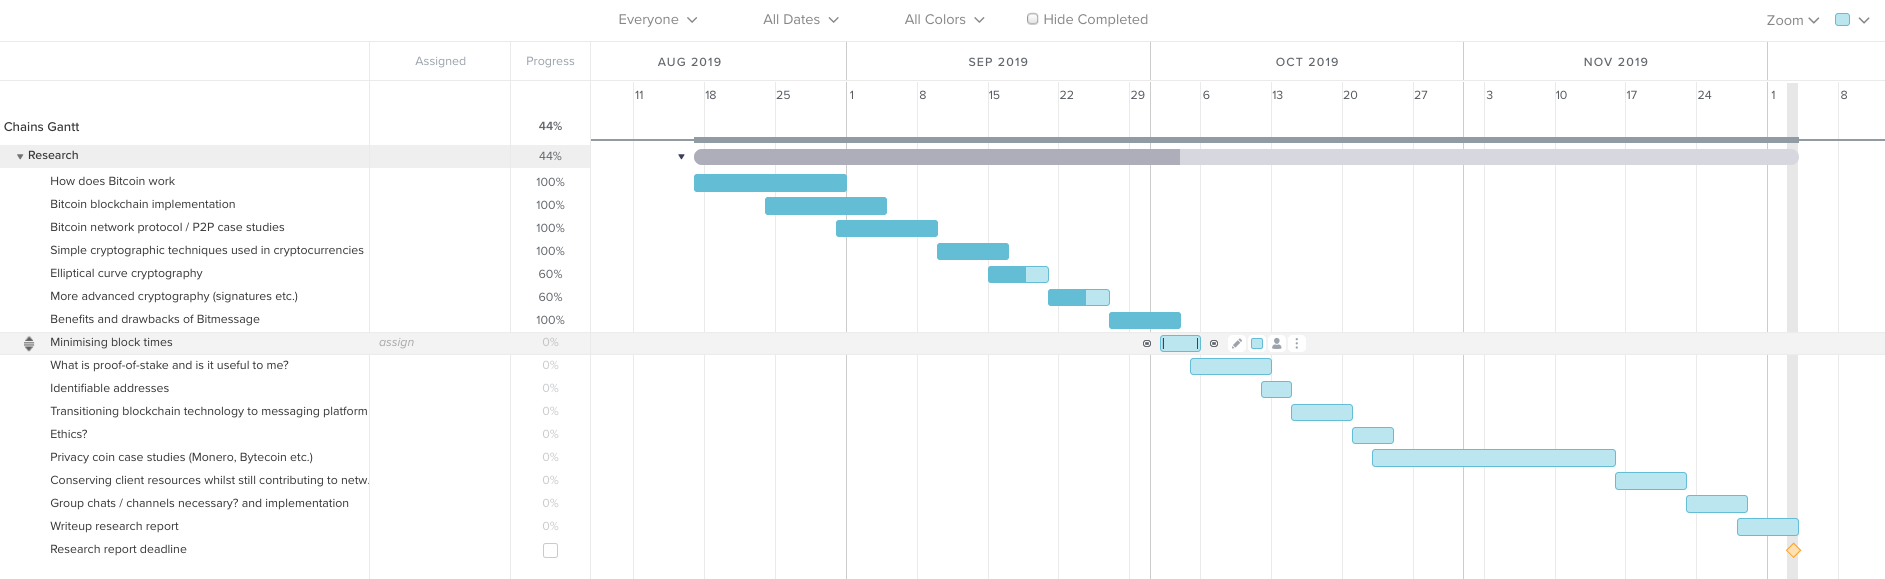
\includegraphics[width=0.9\linewidth]{Images/Gantt_before_ec.png}
    \caption{My original research Gantt chart that I made at the start of the project.}
    \label{fig:ganttbefore}
\end{figure}
\begin{figure}[h]
    \centering
    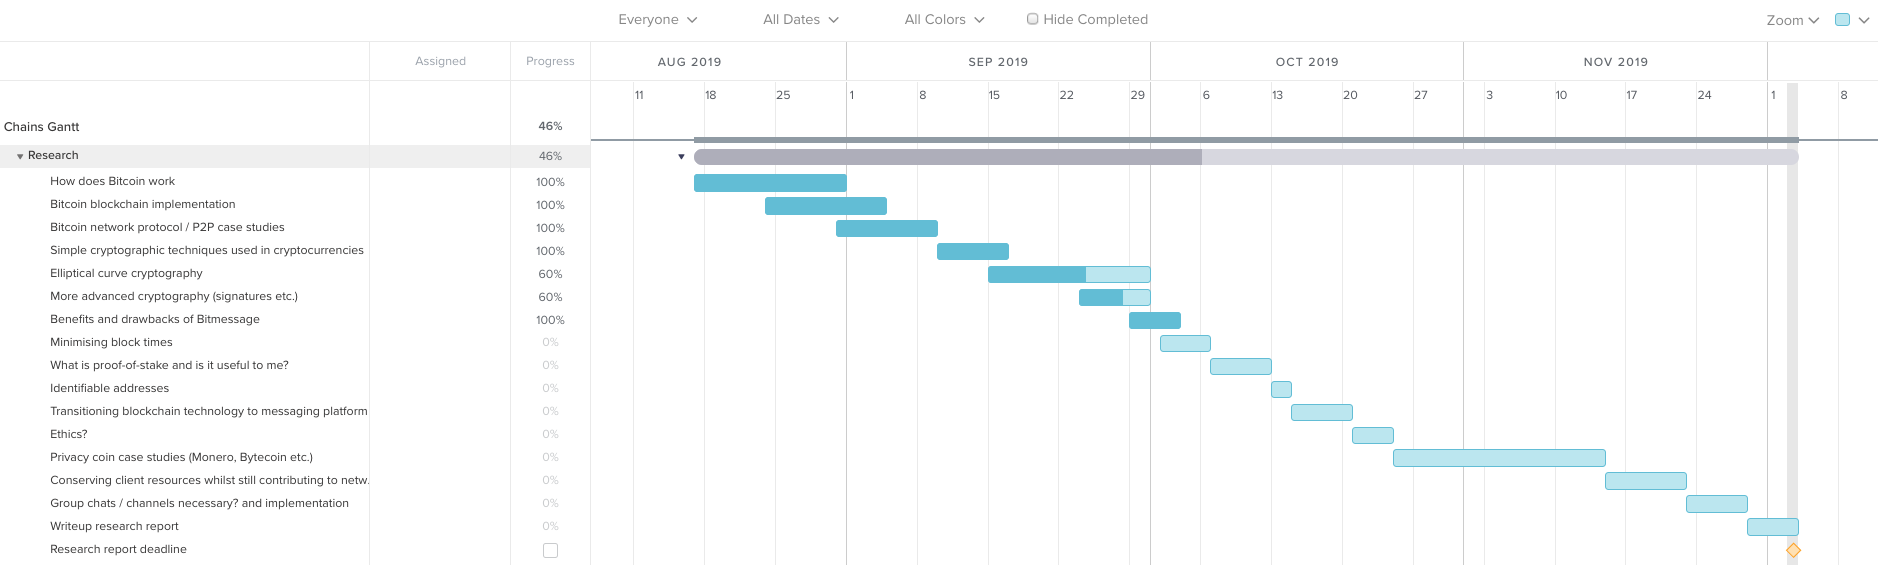
\includegraphics[width=0.9\linewidth]{Images/Gantt_after_ec.png}
    \caption{My research Gantt chart, modified after having realised that Elliptic curve cryptography is a much more complex topic than I previously thought.}
    \label{fig:terec}
\end{figure}

The day after the deadline, I realised that I had neglected to properly discuss ``Minimising Block Times'' which is an important but small part of the project.
\begin{figure}[h]
    \centering
    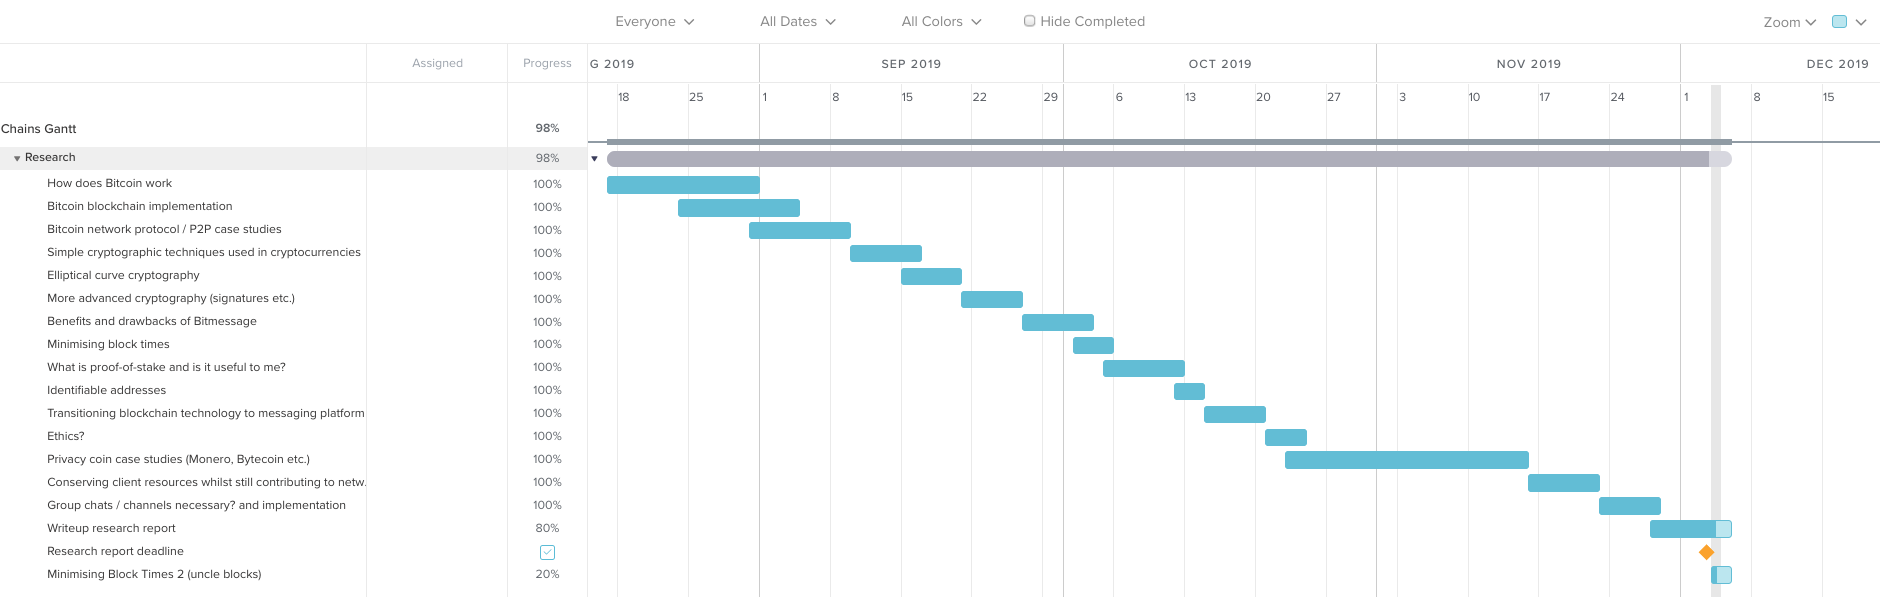
\includegraphics[width=0.9\linewidth]{Images/Gantt_after_uncle.png}
    \caption{My research Gantt chart, modified after having realised that I had not properly discussed ``Minimising Block Times'' in my write-up.}
    \label{fig:teruncle}
\end{figure}
\newpage


\subsection{Why Blockchain?}
The vast majority of messaging platforms at the moment utilise a simple client-server model to allow communication between users. Although this works well for a messaging system, it has several arguably major drawbacks which will be discussed in the next few pages.

\subsubsection{Messaging Case Study - Facebook Messenger / Whatsapp}
Both Facebook Messenger and Whatsapp are feature-packed messaging apps that provide the user with an excellent messaging platform allowing users to quickly and reliably communicate. Globally, over a billion people use Whatsapp or Facebook Messenger every month, making these 2 platforms the most popular of any in the world.
\begin{figure}[h]
    \centering
    
\includegraphics[width=0.4\linewidth]{Images/fbmsgwhtspp.jpeg}
    \caption{Facebook messenger (left) and Whatsapp (right) are the two leading messaging platforms globally.}
    \label{fig:fbmsgwhtspp}
\end{figure}
However, they rely on the client-server model. This means that all messages are stored on servers in a data-centre. Even though these companies say that all messages are encrypted, it is not guaranteed that they are. In fact, many people believe that the USA's National Security Agency (and other nations' government agencies) has been granted `backdoors' into the platforms. This would potentially allow authorities to spy on the general population and results in the loss of privacy for billions of people. I strongly disagree with even the possibility of this being the case as I value my privacy greatly. I believe that everyone should have access to free-speech and privacy.
Also, storing users' data on servers poses a security risk since most of these platforms are completely proprietary and not open source. Servers could potentially be hacked leading to the distribution of user data across illegal forums and marketplaces. This could happen without even the companies' knowledge and bypasses any GDPR data regulations. This shows that these platforms, whilst feature-packed and easy-to-use, are not necessarily trustworthy in the current age of privacy and data-protection.

The likes of Facebook Messenger and Whatsapp do introduce a wealth of features that are extremely useful to the average user, not to mention fun, such as message replies; message reactions; the ability to hold votes (polls); and the ability to set nicknames and the chatname.

\subsubsection{Messaging Case Study - Bitmessage}
Bitmessage\cite{bitmessage_paper} is a decentralised messaging platform that runs on a global peer-to-peer network. Messages are each individually encrypted and distributed across the network. Each machine (completely voluntarily) supports the network by echoing new messages to all its known neighbours.
\begin{figure}[h]
    \centering
    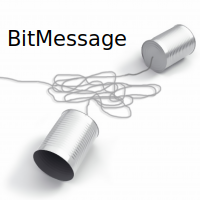
\includegraphics[width=0.4\linewidth]{Images/bitmessagelogo}
    \caption{Bitmessage is a far lesser known alternative to the messaging platforms of today with a focus on privacy.}
    \label{fig:bitmessagelogo}
\end{figure}
I think that the idea of Bitmessage is very strong, managing to achieve pseudonymity through a decentralised network. This means that, similar to Bitcoin, the addresses of users on the network are not linked to identities. However, unlike Bitcoin, there is no single source of truth. This means that when a user wants to check if they have received any messages, they download a message-pool (a large-group of cached messages) from some of their peers on the network and check for any which were created using their public key. This means that the sender cannot confirm for certain that the recipient will have access to the sent message and can only hope that that the message makes its way across the network. Although this is not a platform-breaking issue, it could be very significant in situations that rely on reliable, consistent messaging.

One of the great inventions of the Bitmessage platform is the idea of computational proof-of-work for individual messages. This effectively eliminates spam on the network by making every message require the sender to give up computational resources (users who try to overload the network with messages will have to dedicate unreasonable amounts of computational power to the creation of large quantities of messages).

However, another downside of Bitmessage is the slow propagation delay. Bitmessage is often likened to email due to the way it has been implemented. Messages are treated like emails rather than a persistent instant chat. This means that correspondence with recipients could be slow and disjointed.

\subsubsection{Blockchain Case Study - Bitcoin}
Bitcoin\cite{bitcoin_paper} is the first notable implementation of blockchain technology and was the first blockchain-based cryptocurrency ever. It is useful to examine Bitcoin as one can see the design decisions behind the architecture of a cryptocurrency. Since nearly all other cryptocurrencies adapt their system from Bitcoin in some way, this gives a good view of the basis for a cryptocurrency and how a blockchain could work effectively. It is also simpler than many other cryptocurrencies making it easier to investigate and understand. Bitcoin has become so popular that many shops around the world now accept the currency in shops IRL (see \autoref{fig:bitcoinacceptedhere}) and not just on the internet.
\begin{figure}[h]
    \centering
    
\includegraphics[width=0.5\linewidth]{Images/bitcoin_accepted_here.png}
    \caption{A sign created for sellers to show acceptance of bitcoin as payment method}
    \label{fig:bitcoinacceptedhere}
\end{figure}
For its time, bitcoin was innovative in its privacy for users. It circumvented the need for accounts like PayPal and Stripe have today. It did this using some interesting cryptography that allowed for trustless interaction. However, the Bitcoin blockchain is vulnerable to so-called ``blockchain-analysis''. This entails some users tracing and cross-referencing transactions and addresses over a long period, eventually resulting in compromised user identities. This practice could be carried out by governments or private agencies to bypass the layer of anonymity that stands in-between user's and their wallet addresses. This layer of psuedo-anonymity is known as pseudonymity and has since been deemed less-than-private by the privacy-oriented end of the cryptocurrency community.

\newpage

\subsubsection{Blockchain Case Study - Monero}
Monero (built on Cryptonote\cite{cryptonote_paper}) is currently (as of Nov. 2019) the most popular of all the so-called ``privacy coins''. Cryptonote and consequently Monero are built with the premise of true-anonymity in mind. They utilise some more complex cryptography in order to hide the addresses of senders and recipients. This involves ``stealth-addresses'', which are alias addresses used by the recipient of a payment, and ring signatures which preserve the identity of the message sender whilst simultaneously hiding the quantity of currency in each transaction (Ring Confidential Transactions).
\begin{figure}[h]
    \centering
    
\includegraphics[width=0.4\linewidth]{Images/monerologo.png}
    \caption{The Monero logo}
    \label{fig:monerologo}
\end{figure}
In terms of using the payment framework itself, the currency is just as easy for users to use as Bitcoin. Monero is probably the most well-backed privacy coin with the best documentation\footnote{\hyperlink{GetMonero.org}{\textbf{The official Monero website}} has many videos and blog posts explaining all the aspects of the currency.}.

The Monero Project has also kick-started The Kovri Project\cite{kovri_repo}. This is a new system for routing and encrypting network traffic in peer-to-peer networks such as Monero's. This could be useful to my project as the security of the network is theoretically nearly as important as the security of the blockchain/ledger itself.

\subsubsection{Blockchain as a Solution}
A blockchain would provide a single source of truth for all messages on the network meaning that, for the most part, all machines on the network will be in agreement over all messages. This means that there should never be a situation where a message is lost before it is accessible to the recipient so long as the message makes it into the blockchain in the first place. Blockchains are effective for this solution because they group together message `transactions' making a shared database that anyone can access and anyone can store for as long as they wish. Blockchain does have some downsides however. For example, they are not really designed to work at high block frequency (more blocks found per minute) and will become inherently less secure when at the higher speeds required for an instant messaging service. This will need to be addressed later on if this service is to be considered properly secure.

This system means that individual mobile devices can store the blockchain on their hard drives and be sure of its authenticity to a great deal of certainty. This does, however, introduce the problem of scalability as storing a ledger of all messages ever sent on the network will quickly become impractical.

\subsection{What is (a) Blockchain?}\label{subsubsec:whatisablockchain}
A blockchain is essentially a database that stores a set of grouped records (rows in a data set). These groups of records are known as blocks and each record is typically some form of transaction (in the case of cryptocurrencies, these are monetary transactions). However, it should be noted that these records could be used for a multitude of different uses including digital electoral votes; gambling bets; and medical records. Each block of records contains a reference to the previous block, creating a chain.

Blockchains are most useful when distributed between many computers on a network. This is because they can be combined with some cryptography to allow for trustless interaction between users of the blockchain. The concept of trustless interaction with blockchains is explained well in a blog-post from 2018\cite{medium_trustless_blockchain}. The classic example for this is the transfer of money between two parties. 
\begin{figure}[h]
    \centering
    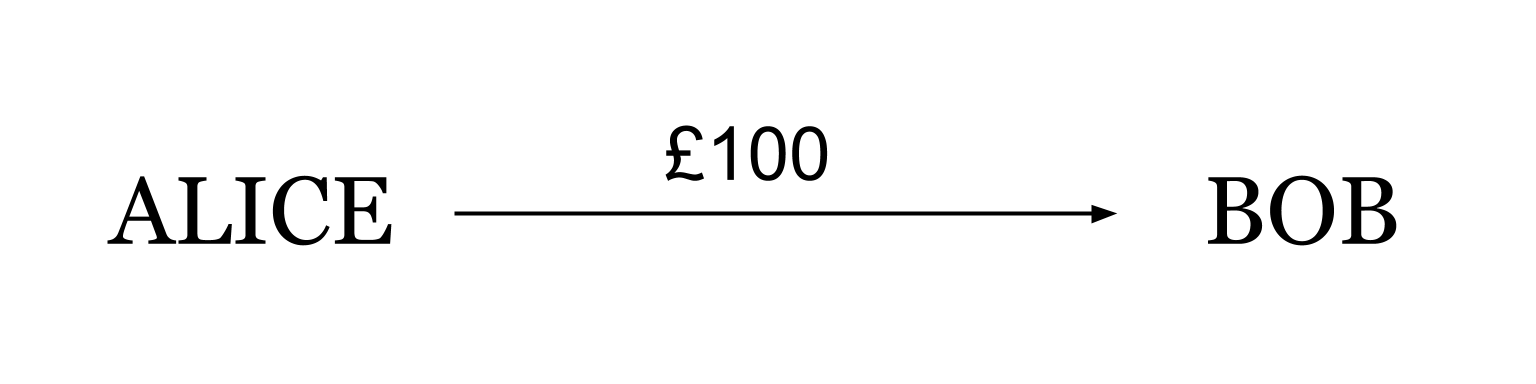
\includegraphics[width=0.65\linewidth]{Images/Diagrams/transaction_in_person.png}
    \caption{Alice gives £100 to Bob in person}
    \label{fig:transactionwoip}
\end{figure}
As explained in the blog-post, the easiest and simplest way to transfer money would be for the two parties to meet in person and trade physical money (see \autoref{fig:transactionwoip}). However, this is not always possible for people who are in either remote location or for those who don't trust their opposite party. One solution to this is to have a trusted intermediary party (usually a bank) who could facilitate the transaction (see \autoref{fig:transactionwip}). 
\begin{figure}[h]
    \centering
    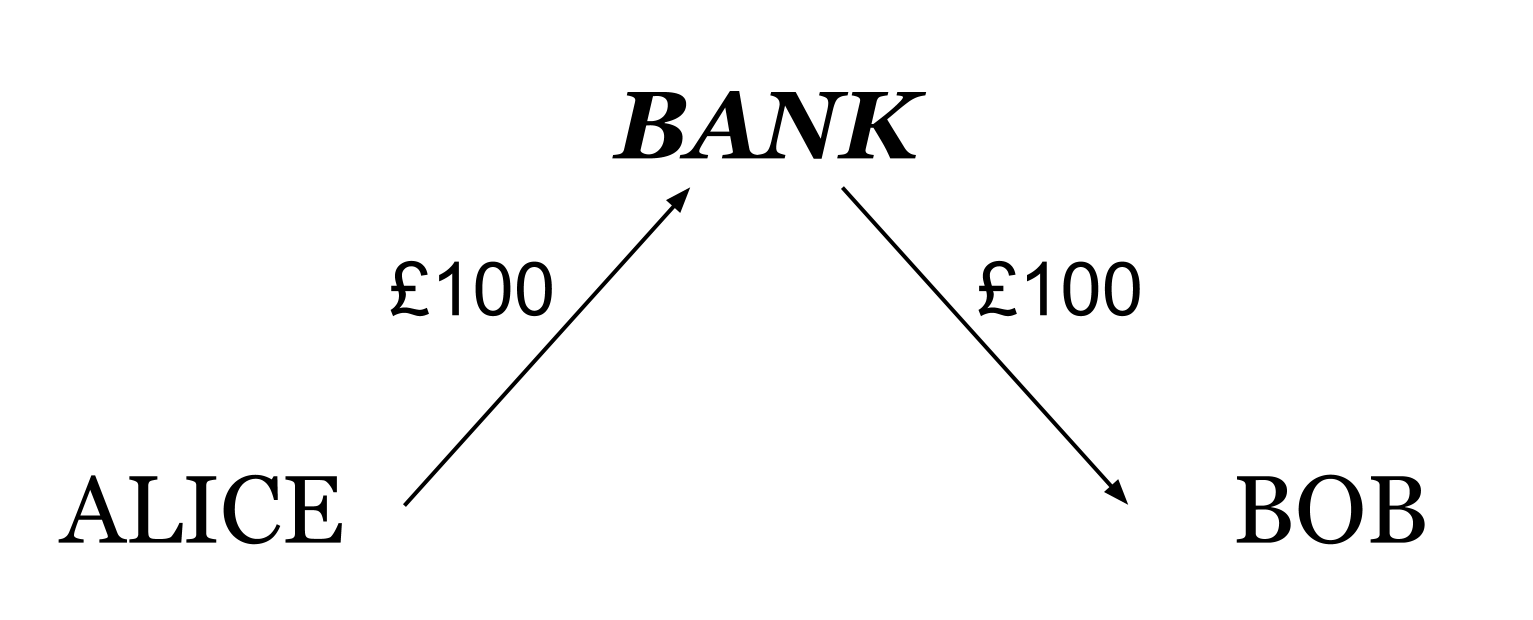
\includegraphics[width=0.65\linewidth]{Images/Diagrams/transaction_with_intermediary.png}
    \caption{Alice sends £100 to Bob through an intermediary party}
    \label{fig:transactionwip}
\end{figure}
This is ideal in the sense that both parties can safely partake in transactions without the drawbacks of meeting up in person. This solution is the most popular of all and is well-established in the global economy. However, once again, there are several drawbacks associated with this form of transaction. Firstly, how can a party be absolutely sure that their intermediary party is in fact trustworthy. This can become quite problematic when large sums of money are being transacted. Also most intermediary parties (banks) are obligated to decline the facilitation of transactions that are believed to be illegally premised or against their wishes. Moreover, if a bank logs all of its transactions, then the private data of users can be hoarded and sold on for the intermediary's profit. As well as this, if the intermediary party were to shutdown or go bankrupt, then users' money could be lost altogether and transactions would fail. Cryptocurrencies solve this problem by replacing the intermediary party with a blockchain.
\begin{figure}[h]
    \centering
    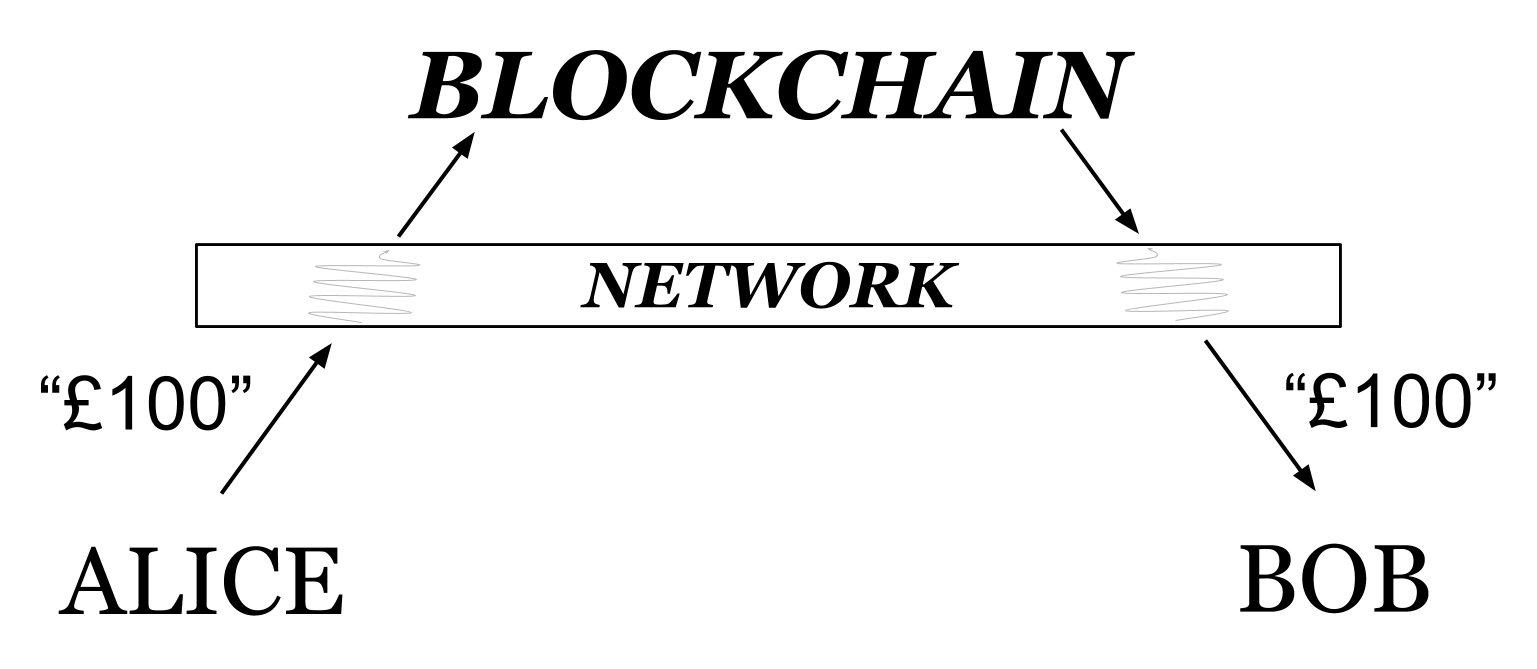
\includegraphics[width=0.65\linewidth]{Images/Diagrams/transaction_with_blockchain.png}
    \caption{Alice sends £100 by means of a blockchain}
    \label{fig:transactionwbc}
\end{figure}
Instead of sending payments to a bank (or other intermediary), a user would declare to a network of listening computers that they wish to make a payment and these computers would record it in the blockchain (see \autoref{fig:transactionwbc}).
These nodes (computers) on the network would always validate a transaction before allowing it to become part of the blockchain. This way, no one is able spend money that they do not have. The network of computers is always running and all connections are direct internet connections between IP addresses. 
Communication is between peers rather than between client devices and centralised servers and is the reason that the network is known as peer-to-peer (rather than client-server as in most contemporary internet communication, see \autoref{fig:p2pnetwork}). New peers are welcomed to the network at any time and likewise anyone can leave. It should be noted, however, that when only a few peers are online in the network, the network will seem to be slow as many connections are being routed through only a few nodes.
\begin{figure}
    \centering
    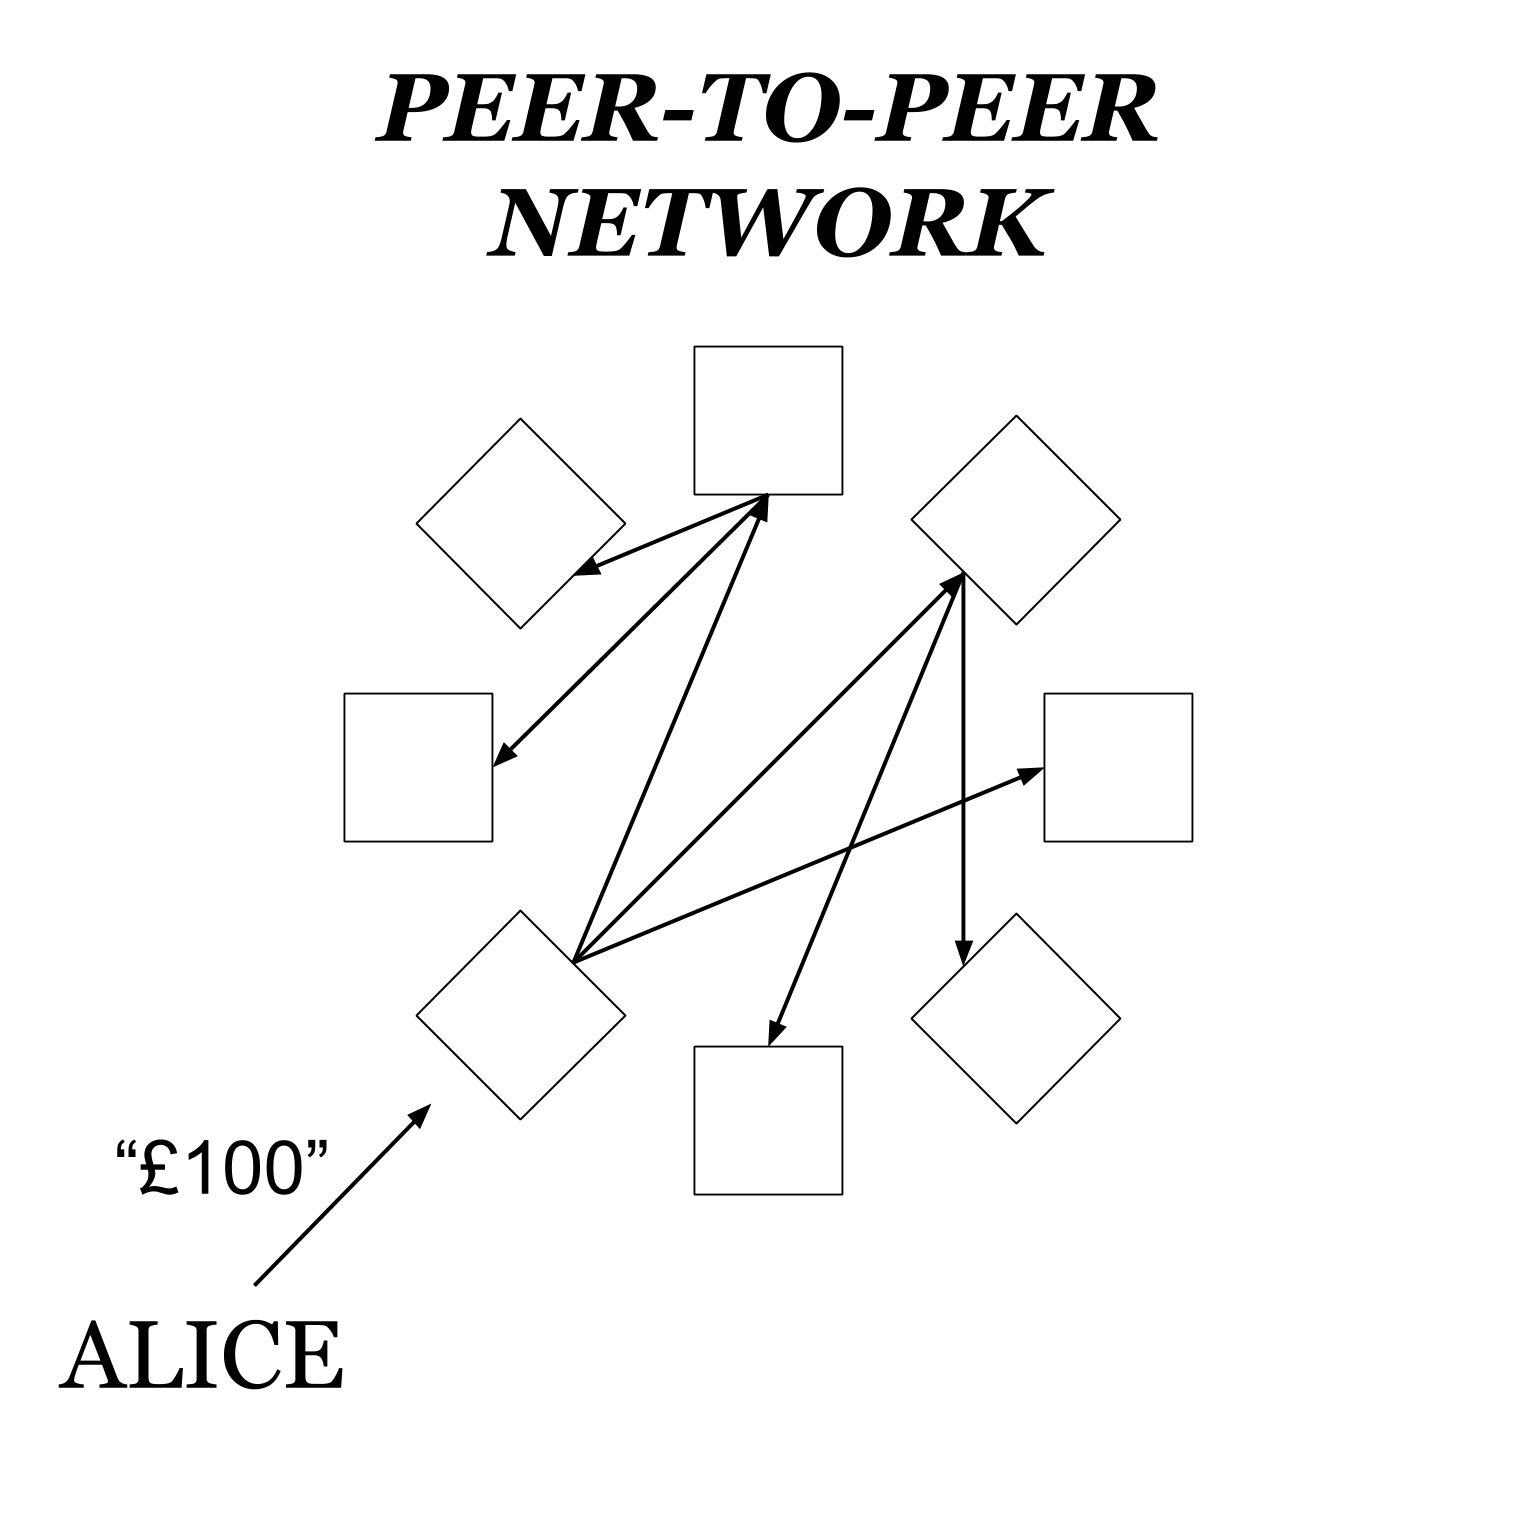
\includegraphics[width=0.5\linewidth]{Images/Diagrams/p2p_network.png}
    \caption{Alice sends the details of her transaction into the peer-to-peer network}
    \label{fig:p2pnetwork}
\end{figure}

When computers on the network receive a transaction, they first confirm the validity of the transaction against the user's previous outputs (received payments, this is a way of checking wallet balance). They then group this with a large number of other recently received transactions between other parties. They then attempt to solve a mathematical puzzle known as a proof-of-work (first proposed for the blockchain in the Bitcoin white paper\cite{bitcoin_paper}). All the nodes on the network will use their computational power to try to break the puzzle and the first one to do so will broadcast their found block to the network. This newly created block contains all the transactions that the solver grouped in the previous step and also the solution to the puzzle. This allows anyone on the network to validate the block by quickly checking if the solution is correct. If a node validates the block, it will add it to its copy of the blockchain. If not, then the node will reject it. The difficulty of the puzzle is adjusted every so often to make sure that the time between blocks being 'found' (the moment when a solution is found to a puzzle and the block is posted) is fairly constant (in Bitcoin and Monero's case, the block-times are around 10 minutes and 10--20 seconds respectively). Nodes on the network follow strict communication rules known as the network protocol (Bitcoin\cite{bitcoin_docs} and Bitmessage\cite{bitmessage_docs}).

Since every block on the blockchain points to the block that came before it, the longest chain of blocks is assumed to be truth. This chain has had the most computational work put into it, since the most puzzles have been solved and thus is most likely to be truth. The longer the chain, the more secure users can be in the knowledge that their transactions are safe. Traditionally (in Bitcoin, Monero and other cryptocurrencies), these nodes are rewarded for dedicating their computing power towards supporting the network. This reward consists of a new piece of currency and is how new ``coins'' are introduced into the system.

\newpage

\subsubsection{Scalability}
One of the greatest benefits of a peer-to-peer network is that it should become faster to use as more nodes join the network. This is very different to the client-server paradigm where companies are forced to spend more and more money on server infrastructure as network traffic increases.

However, pushing updates to servers is often a much easier task than persuading a global peer-to-peer network to do the same. This means that updates will often take longer (normally over a period of months, for example Bitmessage took over a month to upgrade its network to ``protocol v3''\cite{bitmessage_protocol_v3}). This could be a security issue if an exploit is found in the given protocol specification for a network. This means that great care must be taken when devising a network protocol.

Scalability was also a problem in the case of Bitmessage because of the way in which a user finds messages addressed to him; Bitmessage, requires every user to scan through all messages on the network attempting to decrypt every one until one is successfully decrypted. This could slow down message receipt as more messages enter the network and Bitmessage becomes more popular. However, it would compromise much of the network's anonymity to omit this and this may have to become part of the proposed instant messaging platform.

\subsubsection{Minimising Block Times}
Block times are the mean period of time between two adjacent blocks being discovered. In Bitcoin, the block times were set to be around ten minutes. This means that the difficulty of the mathematical puzzle is dynamically changed to keep the time between blocks fairly constant. The more nodes ``mining'' on the network, the more consistent and stable the block times should be since the difficulty will be higher and the probability of finding a block will be lower and spread out over many ``miners''.

Ethereum\cite{ethereum_intro_paper}, a more modern cryptocurrency than Bitcoin, uses block times of 10--20 seconds which means that the rate of finding blocks is significantly higher. This means that the time it will take for a transaction to enter the blockchain will be significantly lower than that of Bitcoin's. Since instant messaging requires fast communication, the proposed platform will require block times on the order of 10--20 seconds like Ethereum's.

''Difficulty'' in Bitcoin is recalculated every 2016 blocks (see \autoref{fig:bc_diff_eq}).
\begin{figure}[h]
    \[\textrm{difficulty}_{\textrm{new}} = \frac{\textrm{difficulty}_{\textrm{old}} \times (2016\ \textrm{blocks} \times 10\ \textrm{minutes})}{\textrm{total time taken (mins) to mine last 2016 blocks}}\]
    \caption{Equation to calculate difficulty (as deviation from original (1.00)) for Bitcoin.\cite{medium_bt_mystery}}
    \label{fig:bc_diff_eq}
\end{figure}
%new_difficulty = old_difficulty X (2016 blocks X 10 minutes) / (the time took in minutes to mine the last 2016 blocks)

In Ethereum, difficulty is calculated ``on the fly''. This means that the difficulty is recalculated after every block and is constantly changing. This should be a more effective approach for the early stages of a blockchain since the fluctuations in total network hash rate from the norm are much more significant.

Difficulty in Ethereum is recalculated based on the most recent block time (see \autoref{fig:eth_diff_eq}).
\begin{figure}[h]
    \[\textrm{difficulty}_{\textrm{new}} = \textrm{difficulty}_{\textrm{old}}
    \ + \ \left\lfloor\dfrac{\textrm{difficulty}_{\textrm{old}}}{2048}\right\rfloor \times \max\left(1- \left\lfloor \frac{\textrm{block\_time}}{10} \right\rfloor,\ -99\right)\]
    \caption{Equation to calculate Ethereum's difficulty (Homestead release) ignoring the ``difficulty bomb''\cite{medium_bt_mystery}. ``block\_time'' is the difference in timestamps between the two most recently found blocks.}
    \label{fig:eth_diff_eq}
\end{figure}

As discussed at the start of \autoref{subsubsec:whatisablockchain}, nodes have to solve mathematical puzzles for the network to function. For Bitcoin and most other cryptocurrencies, the actual puzzle is defined as taking many hashes (see \autoref{subsubsec:hashfns}) of proposed blocks (each a set of transactions grouped by the node). Every block contains a ``nonce'' value. This is just an integer that is kept in the headers. This nonce is incremented after every hash calculation. If the hash of the block with the nonce was less than (or equal to) a specified target, then the block is valid and can be broadcast to the network. If it is greater than the specified target, then the nonce is incremented and the process repeated until either the target is met or a found block is received from the network. This process becomes very resource-intensive at high speeds so machines with a greater hash rate (processing speed) will be able to, on average, calculate more blocks over a period of time. This is known as ``mining'' and was first discussed (for blockchain) in Satoshi Nakamoto's Bitcoin proposal\cite{bitcoin_paper}. In Bitcoin, the network is so full of high hash-rate miners that it is no longer even remotely profitable to mine on a typical desktop machine. Other cryptocurrencies choose to implement hash functions that favour the processors available in more accessible machines (Monero uses the Cryptonight algorithm\cite{cryptonight_docs} which favours the CPU over high-power GPUs and so-called ASICS---Application-specific integrated circuit).

To calculate the target value, it is as simple as scaling the previous target according to the new difficulty (see \autoref{fig:target_eq}).
\begin{figure}[h]
    \[\textrm{target}_{\textrm{new}} = \frac{\textrm{target}_{\textrm{old}}} {\textrm{difficulty}_{\textrm{new}}}\]
    \caption{Equation to calculate target value from current and previous difficulties.}
    \label{fig:target_eq}
\end{figure}
This algorithm should theoretically not `care' about the initial target chosen so long as it is reasonably low difficulty (the system should self stabilise). 

%block_time=current_block_timestamp — parent_block_timestamp
%current_block_difficulty = parent_block_difficulty + (parent_block_difficulty // 2048) * max(1 — (block_time// 10), -99) + int(2**((current_block_number // 100000) — 2))


%new_target = old_target / new_difficulty


\paragraph{GHOST protocol \& Uncle Blocks}\label{para:ghostprotocol}
Blockchains become inherently less secure when block times are low and this was the reason that Satoshi Nakamoto chose 10 minutes for Bitcoin rather than something much shorter. However, as previously mentioned, Ethereum's block times are significantly shorter (10--20 seconds). The topic of minimising block times is explained well by the creator of Ethereum, Vitalik Buterin, in a blog post\cite{toward_twelve_s_bt}. The reason that security suffers at lower block times is the network propagation delay. Network propagation delay is the length of time between a found-block being broadcast and it being received by all\footnote{usually it is more useful to discuss 95\% of the network, rather than 100\% since the last 5\% are often \emph{very} slow.} of the network. As discussed in Bitcoin's proposal paper\cite{bitcoin_paper}, we can calculate the probability of an attacker having control of the network.

Take, for example, a blockchain on a network $N$ of the following properties:
\begin{align*}
    p &\coloneqq \textrm{probability an honest node finds the next block} \\
    q &\coloneqq \textrm{probability the attacker finds the next block} \\
    q_{z} &\coloneqq \textrm{probability the attacker will ever catch up from z blocks behind} \\
    D &\coloneqq \textrm{Network propagation delay} \\
    t_b &\coloneqq \textrm{Expected block time}
\end{align*}

If we consider the case where there is no propagation delay (ie. $D = 0$), then:
\[
q_z = 
\begin{cases}
    1                           &\textrm{if } p \leq q \\
    \left(\frac{q}{p}\right)^z  &\textrm{else}
\end{cases}
\]

As the attacker gets further behind on his parallel version of the blockchain, it becomes exponentially less likely that he will ever catch up. When not taking into account the propagation delay of the network, the blockchain can be modelled very simply. It is simply a series of successive blocks where each references the last (see \autoref{fig:blockchain_no_pdelay}).
\begin{figure}[h]
    \centering
    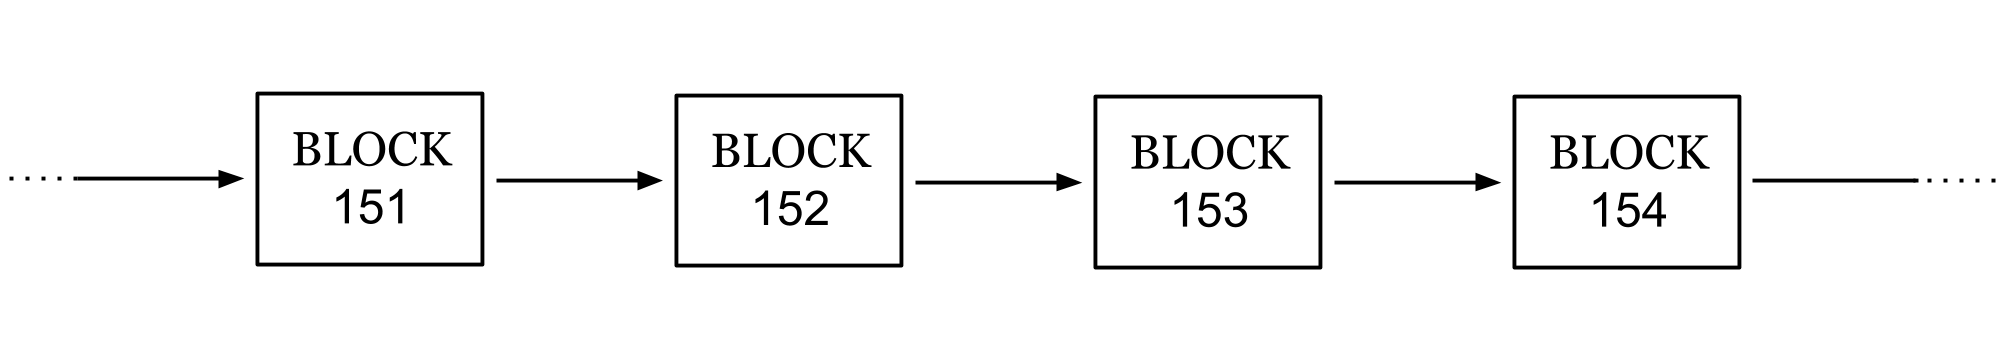
\includegraphics[width=0.9\linewidth]{Images/Diagrams/blockchain_no_pdelay.png}
    \caption{Simple model of a blockchain (not taking network propagation delay into account). Note that the arrows are reversed to show the child of a block rather than the referenced parent.}
    \label{fig:blockchain_no_pdelay}
\end{figure}

The issues of low block times arise when propagation delay \emph{is} taken into account. Now consider a network with a network propagation delay $D = 1$ minute and a expected block time $t_b = 10$ minutes. In such a network, every found block will take 1 minute to reach every node on the network. This means that another node, somewhere on the network, may continue mining for a minute longer than the first person to find the block. This also means that they may find a block before they receive knowledge of any other blocks (see \autoref{fig:blockchain_w_pdelay}). This block is known as a ``stale'' since some of the nodes on the network are aware of a block with an earlier timestamp. This introduces a weakness in the security of the blockchain as a whole because now an attacker is not required to have a majority in hash rate of the whole network.

\begin{figure}[h]
    \centering
    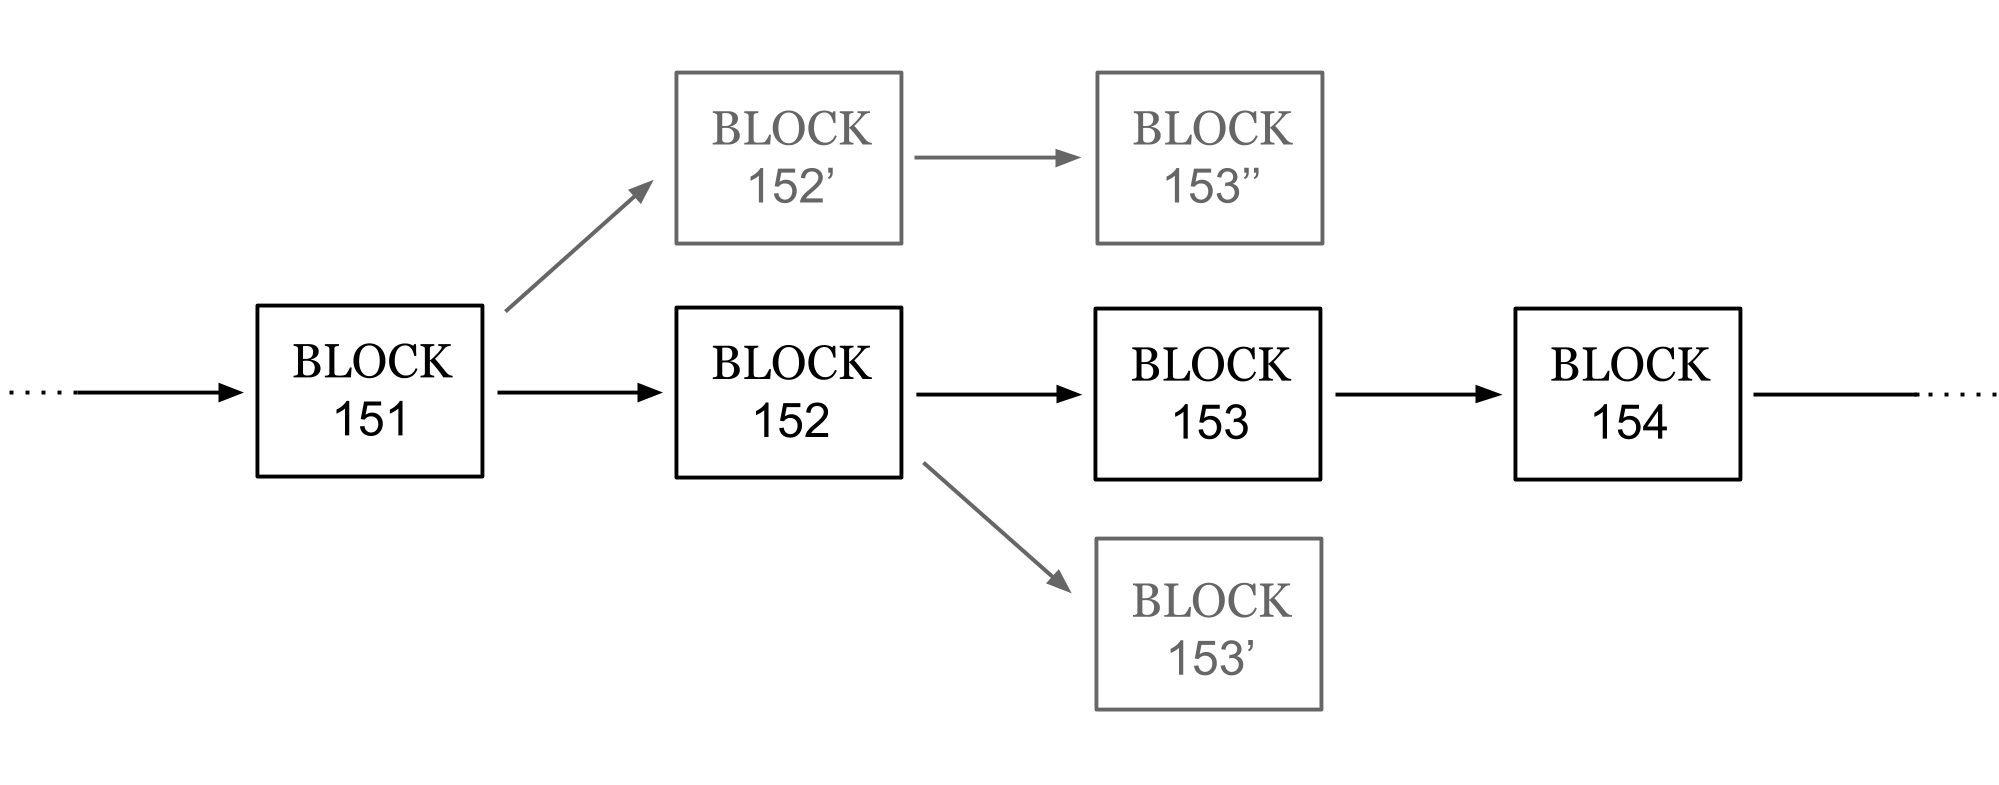
\includegraphics[width=0.9\linewidth]{Images/Diagrams/blockchain_with_pdelay.png}
    \caption{More complex, realistic model of a blockchain (now taking network propagation delay into account). The faded blocks are so-called ``stale''.}
    \label{fig:blockchain_w_pdelay}
\end{figure}

We can calculate the number of stales per found block simply:
\[\textrm{expected\_stale\_rate} = \frac{D}{t_b} \]

We can also calculate the proportion of the network's computational power which an attacker would need access to in order to launch a 51\% attack\footnote{Ironically, a so-called 51\% attack does not require an attacker to control $\geq$ 50\% of the total hash-rate. This applies to Ethereum \textit{and} Bitcoin, though to lesser extent.}. If the attacker is a single node, then the required proportion of network hash power to control the Bitcoin network would be only 49.5\% assuming a network propagation delay $D$ of 12 seconds\footnote{12 seconds\cite{twelve_s_for_btc} is considered the mean delay in reaching 95\% of the network for bitcoin.}.
\begin{align*}
    \textrm{proportion\_needed} &= \frac{1-\textrm{stale\_rate}} {2-\textrm{stale\_rate}} \\
    &= \frac{1 - (12 / 600)} {2 - (12 / 600)} \\
    &= \frac{0.98}{1.98} \\
    &\approx 0.494 \\
    &\approx 49.5\%
\end{align*}

This can also be applied to Ethereum's network details. Here we assume that no stales are included in the blockchain (just like Bitcoin). Thus this figure is significantly lower than in reality. Again we take $D$ to be $\approx$ 12 seconds.
\begin{align*}
    \textrm{proportion\_needed} &= \frac{1 - (12 / 15)} {2 - (12 / 15)} \\
    &= \frac{0.2}{1.2} \\
    &\approx 0.167 \\
    &\approx 16.7\%
\end{align*}

Here, we can see that, with a single node, the attacker would need to control 16.7\% of the network's total hash rate. Since pools of miners often control upwards of 30\% of some cryptocurrencies' networks, it would be unacceptable to release Ethereum without the introduction of the inclusion of ``uncle blocks'' to maintain a secure, trustless platform. The Ethereum platform rewards those who have mined uncle blocks or included a reference to uncle block(s) and this provides a secondary incentive to mine the coin. This means that the idea of mining stale blocks doesn't result in fewer miners on the network. Ethereum's system for handling uncle blocks bases itself on the Greedy Heaviest Observed Subtree (GHOST) protocol (with some important modifications).

\newpage

\subsection{Cryptography}
Cryptography in computer science is the subject of analysing and creating codes to encrypt data. This is a very important principal feature of all cryptocurrencies and most blockchains. Without cryptography, Bitcoin, Monero and Bitmessage would not be possible. It is an essential building block of trustless interaction and cannot be ignored.

\begin{figure}[h]
    \centering
    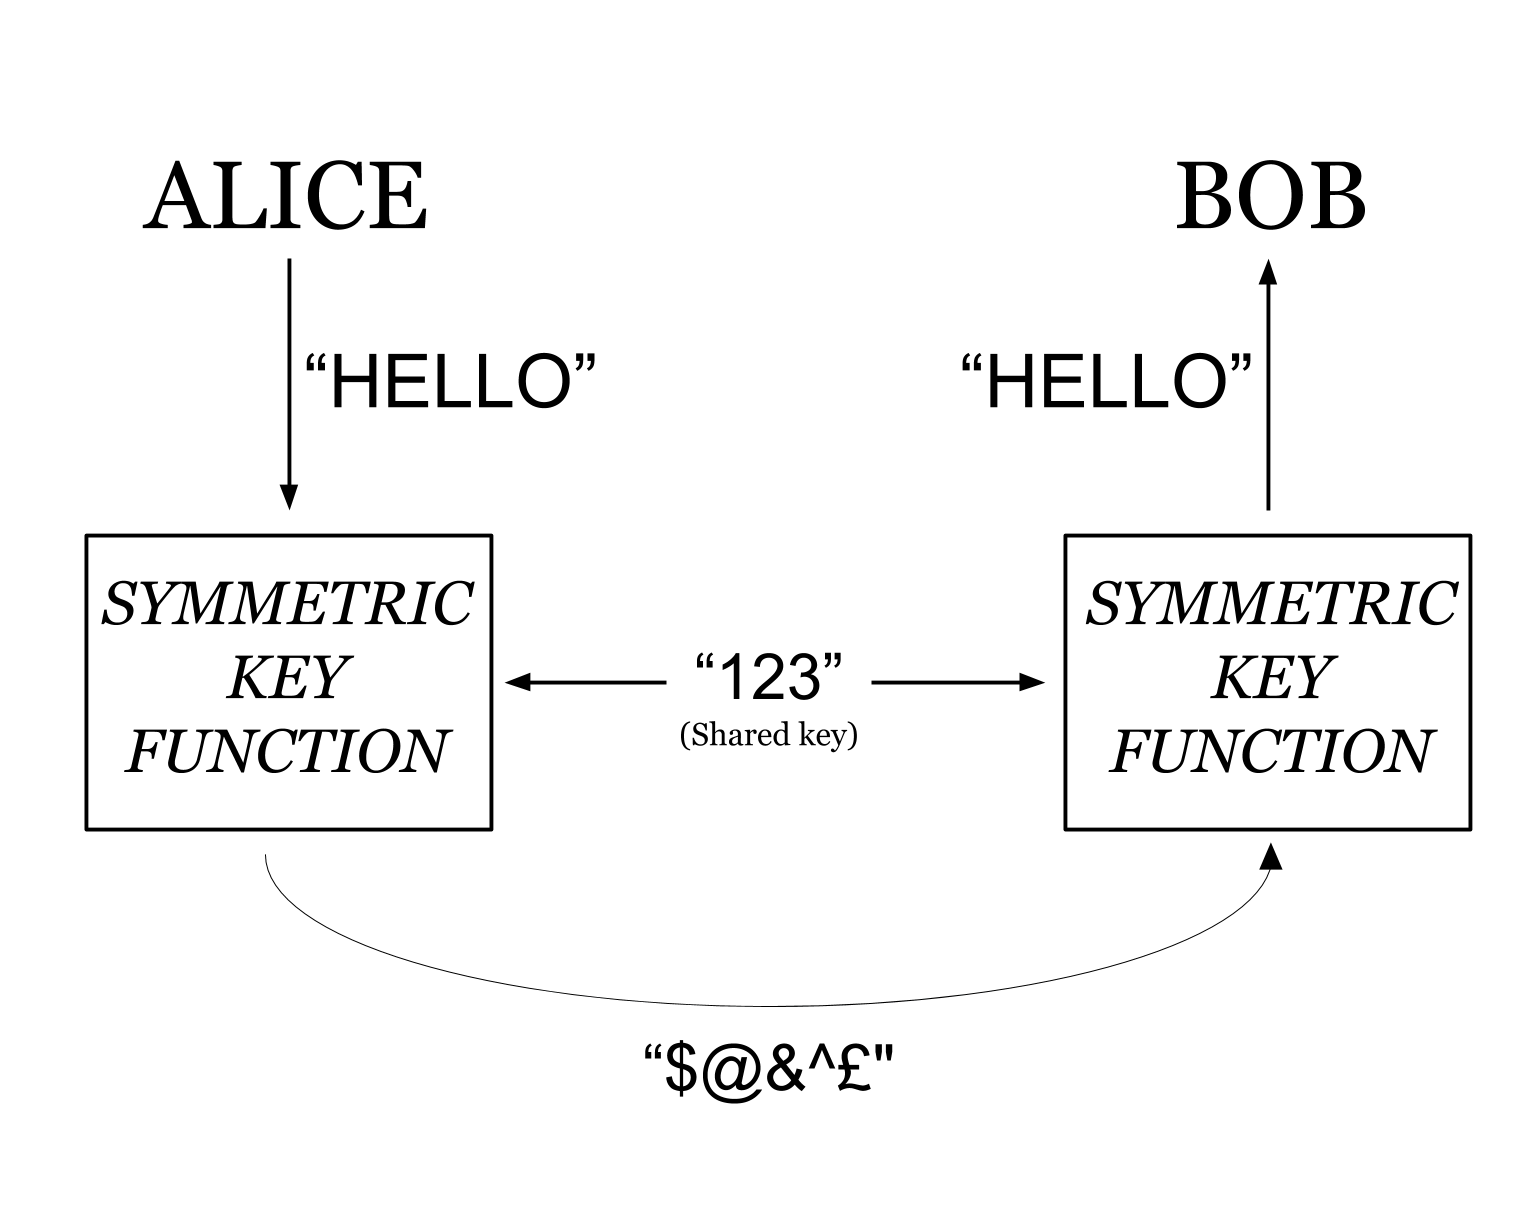
\includegraphics[width=0.5\linewidth]{Images/Diagrams/symmetric_key_encryption.png}
    \caption{Symmetric Key Encryption. Alice encrypts her text with the key 123. The resulting cipher-text is ``\$@\&\textasciicircum£''. Bob decrypts her cipher-text with the key 123. Onlookers are unable to decipher the message without knowledge of this key.}
    \label{fig:symkeyenc}
\end{figure}
\subsubsection{Symmetric Key Encryption}
Symmetric key encryption is the encryption and decryption of data with one shared key (see \autoref{fig:symkeyenc}). This key is known only to the creator/sender of the message-data and its intended recipient.
Examples of this form of encryption include AES\cite{aes}, DES and Blowfish. This form of encryption can be very useful for fast encryption and decryption which is ideal for high traffic situations. It is used extensively for internet traffic secured with TLS (Transport Layer Security). However, it used very little in the context of blockchains and cryptocurrencies.

\subsubsection{Hash Functions} \label{subsubsec:hashfns}
Hash Functions are algorithms that (hopefully) irreversibly 'encrypt' data. They take some input and return a pseudo-random string of data (see \autoref{fig:hashfns}). For most hash functions, the length of output is fixed. Hash Functions are intended to provide a unique output for every input though on very rare occasions, this is not the case. Importantly, they always return the same value given the same input. This means that they can be used for checking data integrity. For example, if someone wanted to make sure that a message did not get corrupted in transit, they could attach a 'hash' (output of hash function given message as an input) of the message to the end of the message. The recipient of the message could then use the same hash function to hash their received message. If his calculated hash is the same as the sender's included hash, when compared, then the message data's integrity has been maintained.
\begin{figure}[h]
    \centering
    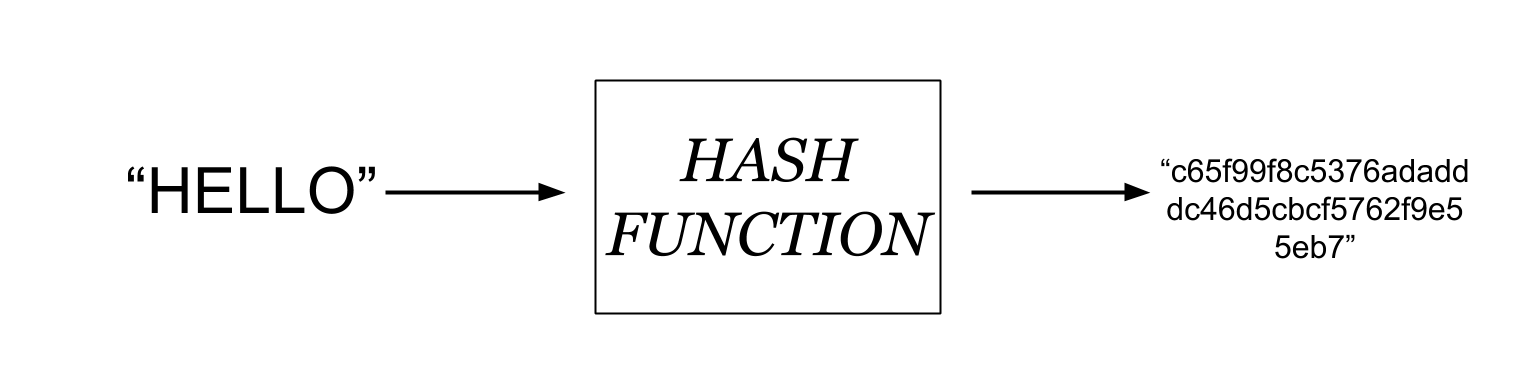
\includegraphics[width=0.8\linewidth]{Images/Diagrams/hash_function.png}
    \caption{Hash Function. In this case the hash function ``SHA-1'' is used to hash the word ``HELLO'' into the following pseudo-random output: ``c65f 99f8 c537 6ada dddc 46d5 cbcf 5762 f9e5 5eb7''}
    \label{fig:hashfns}
\end{figure}

However, it would still be possible for a malicious party to intercept and tamper with a message since they can just recalculate the hash after modifying the message content.

\subsubsection{Asymmetric Key Encryption/Signing}
Asymmetric key encryption is the encryption and decryption of data with two different keys (see \autoref{fig:asymkeyenc}). Typically, one of these keys is known as the public key and the other is known as the private key. The public key is shared around and normally accessible to anyone. The private key is kept secret and is only ever known to the owner of the key. When someone wants to send some data, they encrypt it with the recipient's public key. It is now extremely, computationally difficult for anyone to successfully decrypt the cipher-text unless they have access to the recipient's private key. This form of encryption is one of the methods used by Bitmessage to secure messages. 

Whilst it is computationally easy to derive a public key from a private key, it is extremely computationally difficult to do the reverse. This is the basis for asymmetric keys. The mathematical formulae used to derive the keys utilise the intractability of certain fields of mathematics such as the ``Discrete Logarithm Problem'' to allow for this.

\begin{figure}[H]
    \centering
    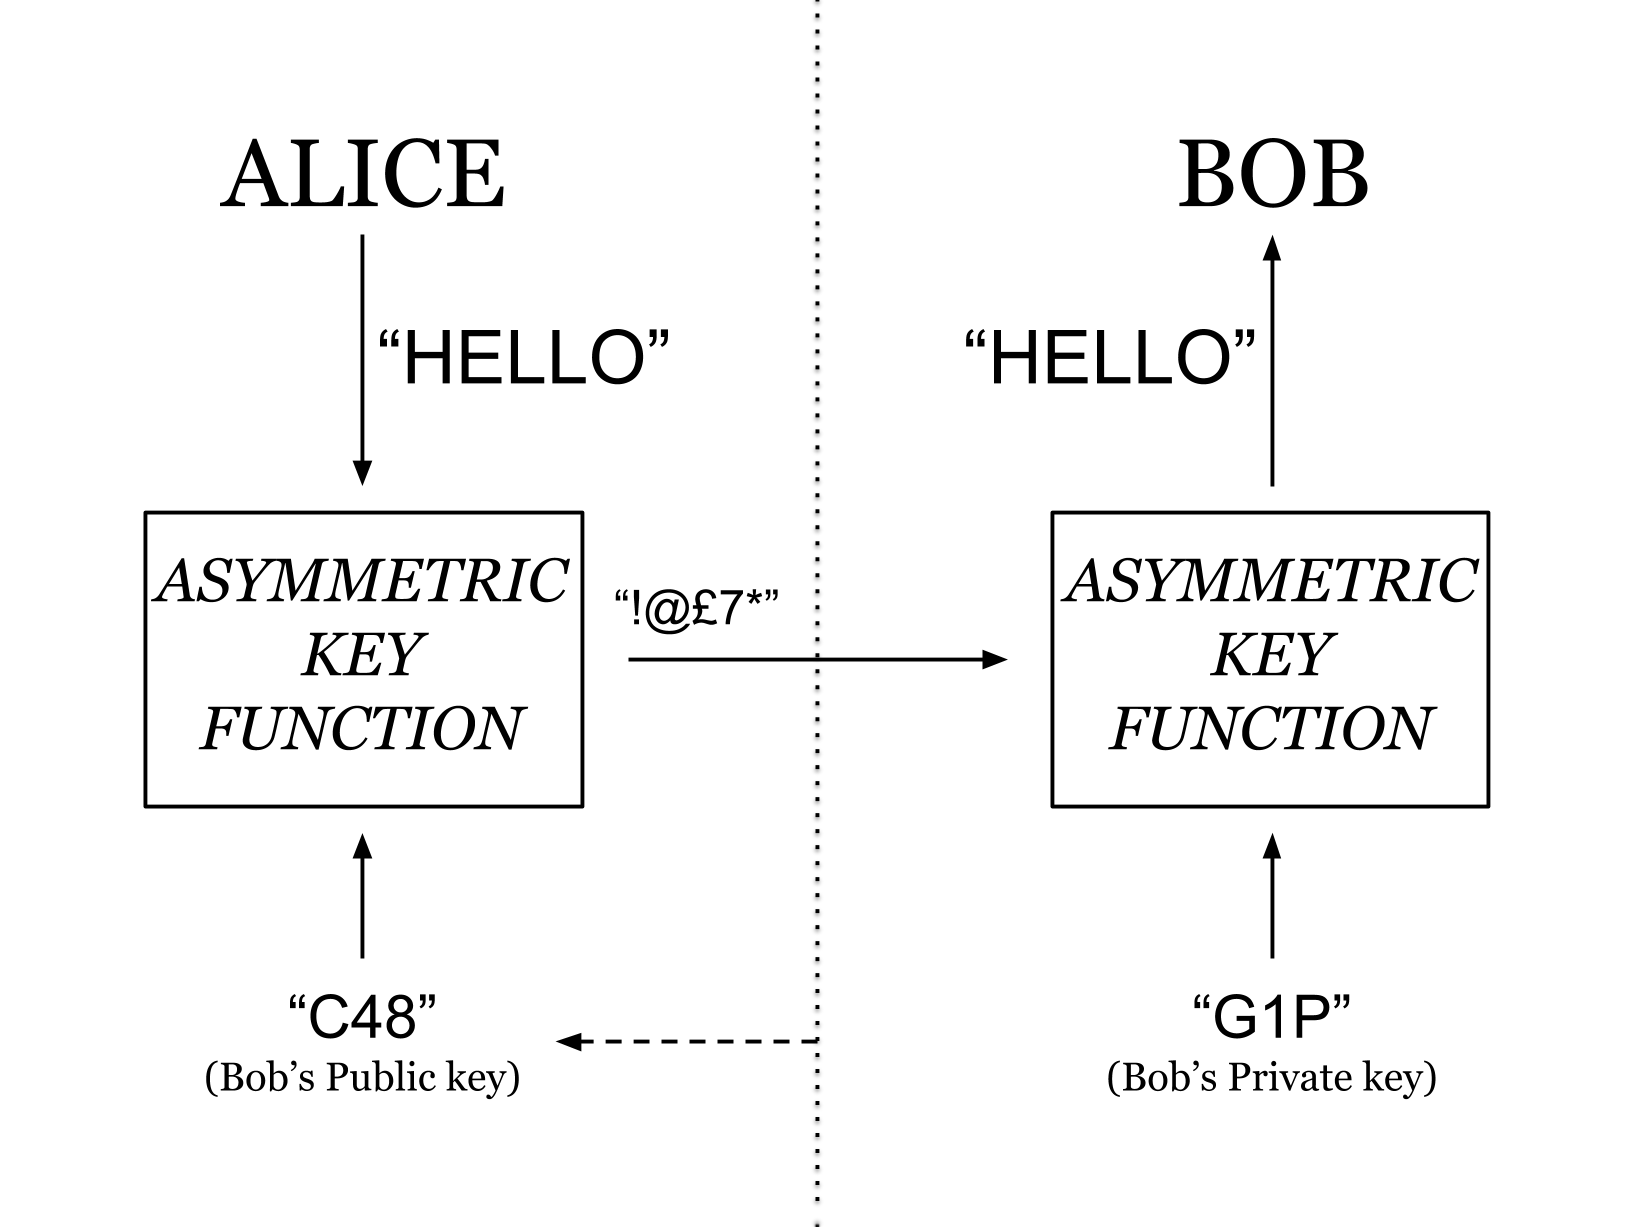
\includegraphics[width=0.6\linewidth]{Images/Diagrams/asymmetric_key_encryption.png}
    \caption{Asymmetric Key Encryption. Alice encrypts her text with Bob's public key C48. The resulting cipher-text is ``!@£7*''. Bob then decrypts Alice's cipher-text with his private key G1P.}
    \label{fig:asymkeyenc}
\end{figure}

Asymmetric key encryption is normally more useful than the symmetric equivalent because it does not require a secret key exchange; no secret information is ever exchanged and therefore there is very little risk of a compromise in security during communication.
Asymmetric key encryption can also be 'reversed' to create asymmetric key signatures (see \autoref{fig:asymkeysig}). A signed message is created by encrypting some data with the sender's private key. It is then only able to be decrypted by the sender's public key. Since this public key is widely accessible to anyone, these allow anyone to verify the sender of the message. This is useful when someone needs to verify the authenticity of the message but the content of the message is intended for public access (data is not encrypted). This is again used extensively in blockchain applications such as Bitcoin and Monero.

\begin{figure}[H]
    \centering
    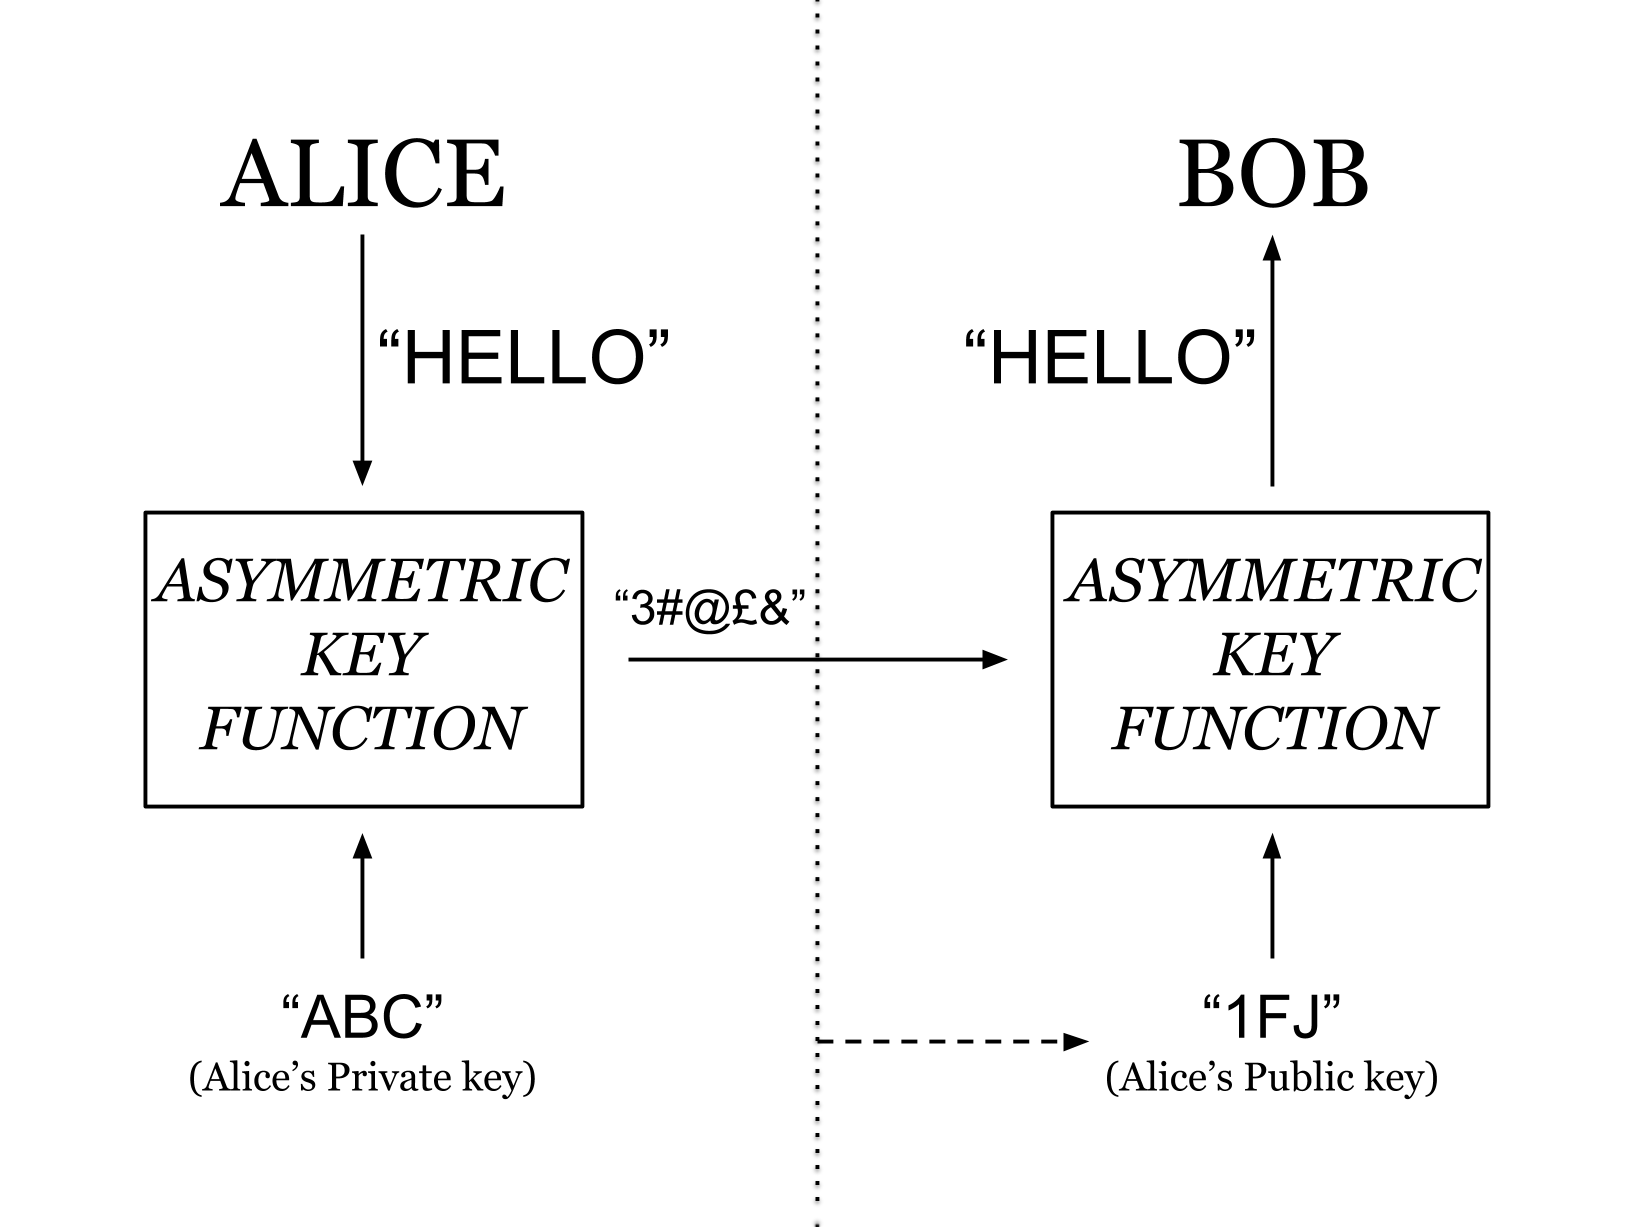
\includegraphics[width=0.6\linewidth]{Images/Diagrams/asymmetric_key_signature.png}
    \caption{Asymmetric Key Signature. Alice encrypts her text with her private key ABC. The resulting cipher-text is ``3\#@£\&''. Bob then decrypts Alice's cipher-text with Alice's public key 1FJ, thereby verifying that Alice is the sender.}
    \label{fig:asymkeysig}
\end{figure}

Examples of Asymmetric key encryption/signature algorithms include RSA, DSA and Elliptic Curve. RSA is an older standard which requires relatively large key sizes to provide a respectable level of security and is therefore not used much in the context of blockchains and cryptocurrencies though is still very popular elsewhere. It relies on the intractability of computing integer factorisation. DSA is a similar standard but only allows for signatures and no encryption or key exchange (DSA relies on the intractability of the Discrete Logarithm Problem).

\subsubsection{Elliptic Curve Cryptography (ECC)}
Elliptic curve cryptography is the encryption system of choice for all contemporary, security-sensitive projects. Here\cite{ic_encryption_course} is a useful guide that I found during research that explains modular arithmetic and finite fields well. ECC is public/private-key based and relies on the computational difficulty of the Elliptic Curve Discrete Logarithm Problem.

\paragraph{Modular Arithmetic}
Modular Arithmetic is used in many asymmetric encryption systems. The idea of modular arithmetic is to work with remainders of divisions. For example: \[9 \equiv 1\ (\textrm{mod}\ 4),\]\[3 \equiv 3\ (\textrm{mod}\ 9)\]{\centering and \par}\[18 \equiv 0\ (\textrm{mod}\ 9)\]

The number 9 is congruent to 1 in (mod 4) space since 9/4 gives remainder 1.

Likewise, 3 is congruent to 3 in (mod 9) space since 3/9 gives remainder 3.

18 is congruent to 0 in (mod 9) space since 18/9 gives remainder 0.

Any integer $r\ (\textrm{mod}\ m)$ can be written as $k*m+r,\ k \in \mathbb{Z}, r \in \mathbb{N}$. Note that, here, $0 \in \mathbb{N}$.

However, one must be careful with negative numbers since although $9 \equiv 1\ (\textrm{mod}\ 4)$, $-9 \not\equiv 1\ (\textrm{mod}\ 4)$. This is because $9=2\times4+1$ but $-9\not=-2\times4+1$. In fact, $-9=-3\times4+3$. Therefore $-9 \equiv 3\ (\textrm{mod}\ 4)$.

Modular arithmetic can also be thought of as a clock face. When the `hours hand' passes through twelve it resets back to one as if the time is constantly being divided by 12 and remainder taken. Modular arithmetic is sometimes also known as `Clock Arithmetic' for this reason.

Performing simple arithmetic operations to numbers in mod space is quite simple. For example, for addition: \[10+2 \equiv 12 \equiv 4\ (\textrm{mod}\ 8)\]This also applies for subtraction: \[10-2 \equiv 8 \equiv 0\ (\textrm{mod}\ 8)\] Multiplication is just as easy: \[10\times 2 \equiv 20 \equiv 4\ (\textrm{mod}\ 8)\]
However, calculating the division of two numbers in mod space is more complex. Division is not defined for every number and division is only allowed to take place if the divisor has a multiplicative inverse (explained well here\cite{ic_encryption_course}, under the modular arithmetic section).

\paragraph{Finite Fields}
To understand how ECC works, it is important to understand finite fields. Finite fields are also explained well here\cite{ic_encryption_course}. A finite field is a group of numbers (with finite length) containing all integers mod $p$ where $p$ is usually a prime number (in this case it is prime). The numbers in the field possess some useful properties:\\
\\Closure:
\[a+b \equiv c\ (\textrm{mod}\ n),\ 0 \leq c \leq n-1\]
Associativity:
\[a\times (b + c) \equiv a\times b + a\times c\ (\textrm{mod}\ n),\ \textrm{for all}\ a,b,c \in \textrm{Field}\]
Contain an Identity element (for $+$ and $\times$):
\[a+0 \equiv 0+a \equiv a\ (\textrm{mod}\ n)\]
\[a\times 1 \equiv 1\times a \equiv a\ (\textrm{mod}\ n)\]

\paragraph{Elliptic Curves}
Elliptic curves are defined as the set of points satisfying the equation $y^2 = x^3+ax+b$ where $4a^3 + 27b^2 \not= 0$ (limited to avoid singular curves). A useful guide that I found on elliptic curve cryptography can be found here\cite{ec_guide}. For cryptography, the curve is defined over a finite, prime field. A single operation is defined for an elliptic curve ($+$). The identity element of the finite field is defined as the point at infinity (written as 0/zero). Here, we are given two points on the curve and are looking for the third (the point that lies on the same line as the other two points as well as the same elliptic curve). If $P,Q,R$ are all defined to be on a line and on the elliptic curve, then the $+$ operation is defined as $P+Q+R=0$. In other words the operation which defines addition in this field takes two points $P,\ Q$ and gives the result $-R$. This is equivalent to finding the mentioned third point and inverting/reflecting it across the x-axis. 
\begin{figure}[h]
    \centering
    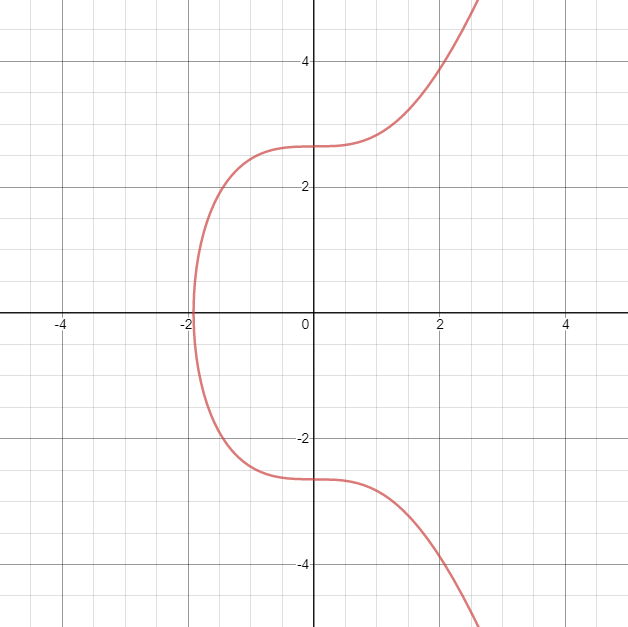
\includegraphics[width=0.5\linewidth]{Images/Secp256k1.png}
    \caption{Elliptic curve secp256k1 $(y^2=x^3+7,\ [a=0,\ b=7])$ over the real numbers. This is the curve used by Bitcoin. Note that when defined over finite field, this would actually look like many scattered points.}
    \label{fig:secp256k1}
\end{figure}

Addition that is repeated many times is said to be the scalar multiplication operation. For example: $nP = P+P+P+P+...+P$, $nP$ is the same as $P$ added to itself $n$ times.
In terms of actually finding the third point on the curve $R=(x_R,\ y_R)$, some algebra can be used:
\[x_R=m^2-x_P-x_Q\ (\textrm{mod}\ p)\]
\[y_R=y_P+m(x_R-x_P)\ (\textrm{mod}\ p)\]
\[\ \ \ \ =y_P+m(x_R-x_Q)\ (\textrm{mod}\ p)\]

If $P\not=Q$:
\[m = (y_P-y_Q)(x_P-x_Q)^{-1}\ (\textrm{mod}\ p)\]

If $P=Q$:
\[m = (3x_P^2 + a)(2y_P)^{-1}\ (\textrm{mod}\ p)\]

In fact, the points that we will use will not all be integers $\leq p$ (where $p$ is prime). This is because, if you take a base-point $G$, then the points $G, 2G, 3G, 4G, 5G... nG$ will form a cyclic subgroup. This means that for example (arbitrary curve parameters) $[G, 2G, 3G]=[4G, 5G, 6G]$. This subgroup will always include zero (the identity element) and so the ``order'' of a base-point is understood to be the number of elements between a base-point and 0. For example, for a base-point $G$, the order of $G$ is the smallest positive integer $n$ for which $nG = 0\ (\textrm{mod}\ p)$. The cofactor $h$ of the subgroup is defined as $N/n$ where $N$ is the order of the elliptic curve and $n$ is the order of the subgroup. $h$ is always an integer since $N$ is a multiple of $n$. This gives us $NP=0$ and therefore $n(hP)=0$. Generally, for cryptography, the base-point is chosen to have a large, prime order.

This gives us 6 parameters for our elliptic curve cryptography algorithm: prime number $p$ (size of finite field), $a$ and $b$ (coefficients in elliptic curve equation), $G$ (a base point that determines the cyclic subgroup), $n$ (the order of the subgroup's order), $h$ (cofactor of subgroup). Sometimes another parameter $S$ is included, this is the seed that can be used to verify that the coefficients $a$ and $b$ are random.

From here we can create a public/private key encryption algorithm. We take the private key to be an integer $d, d \in [1,n-1]$, where $n$ is the subgroup order. We take the public key to be the point $H$ where $H=dG$ and $G$ is the subgroup base-point. This whole algorithm is based around the Discrete Logarithm Problem (it is hard to get $x$ given $P=xQ$ where $P,Q$ are points on the curve).

\paragraph{ECDSA}
ECDSA (Elliptic Curve Digital Signature Algorithm) is the elliptic curve equivalent of the DSA algorithm. It entails taking the hash of some data with a cryptographically-secure hash function. Then signing the hash of the data with the sender's private key. This can then be used as a signature to the message and anyone can verify the authenticity of the message using the sender's public key. This is the signature algorithm used by Bitcoin and most other cryptocurrencies.

\paragraph{Shor's Algorithm}
Although it is computationally intractable for classical computers to compute a private key from a public key, Shor's algorithm reduces the intractability significantly ($\mathcal O(\textrm{log} n)^3$ time complexity) for the same commputation performed on quantum computers. However, contemporary quantum computers are not yet capable of such calculations yet. The moment that they become able to perform such a calculation, the security of much of the internet will cease to be effective.

\newpage

\subsection{Messaging Platform Features}
During research, I collected up all the messaging apps that I considered popular, looking for desirable features that would improve the user experience on my messaging platform. I have devised the following list of features that I would like to be made available:
\begin{itemize}
    \item Group Chats
    \item Stickers
    \item Message Receipt Acknowledgements
    \item Message Reactions
    \item QR Code Addresses
\end{itemize}

\subsubsection{Group Chats}
Group chats are a staple feature of all current, major messaging platforms including Facebook Messenger and Whatsapp. Group chats are chats with multiple people on them rather than just two. However this could be hard to design for and could lead to weaknesses in the security of the platform.

In Bitmessage, the closest thing to a group chat is a ``chan'' or channel. Users subscribe to channel addresses which are just addresses controlled by multiple people. This is the equivalent of an email mailing list (except the recipients decide whether they are on the list rather than the sender).

To implement group chats into my proposed platform, I think I would have a private key for the chat which is shared to all users in the group when created. Each user in the group would use this private ``view'' key to see the contents of the message (similar to Monero's ``view'' and ``spend'' key). They could then use a separate, private ``send'' key to allow them to send messages to the group. Each message to the chat would be required to include a signature (signed with sender's own private ``send'' key) so that the sender of the message can always be determined by others in the group.

\subsubsection{Stickers}
Stickers are a modern modification to typical messaging apps. They are similar to emojis in that they are images as opposed to plain-text. In my opinion, this is best implemented in Apple's iMessage. Stickers are often animated providing a more entertaining and interesting way of chatting with friends. This should be relatively easy to implement as they are just another form of message.

\subsubsection{Message Receipt Acknowledgements}
Older messaging platforms including SMS fail to show a user when their sent message has been received. Again, I think that this is a very important feature as it is very useful to know if your message has been seen. This will be relatively easy to design for but it will be hard to make the feature compulsory (ie. every user has to acknowledge that they have received a message).

\subsubsection{Message Reactions}
Since I have started using Facebook Messenger, I have really enjoyed using the message reaction feature and I think that it adds a lot to the user experience of the platform allowing for more interesting communication. This feature allows the user to 'react' to a message on a chat with a small animated emoji (usually laughing or crying). It would also be important to include the ability to reply to messages with more messages. This could be quite easy to design for since, again, it is just another form of message.

\subsubsection{QR Code Addresses}\label{subsubsec:qrcodes}
Although perhaps underused, Snapchat has a feature known as Snapcodes that allow a friend to quickly add them as a friend. All they have to do is scan the code and the app does all the work. This would be an important feature of the proposed platform since addresses will probably be unwieldy and hard to remember (long strings of seemingly-random characters). This should be fairly easy to design for since it is easy to convert a string of characters into a QR code.

\subsubsection{Minimising Storage/Computation for Clients}
It will be important to manage client resource requirements carefully (for example, client devices like mobile phones should not need to store 120GB of blockchain all the time as this is impractical and would be unpopular). To address the problem of limited client storage resources, I have researched into the feasibility of the following solution. All ``semi-thin'' clients (typically anyone's smartphone who has the app) will only store a random portion of the blockchain. This random portion will be small but with enough devices on the network, this should mean that no blocks are lost from the network entirely. All ``full-node'' clients will store the entire blockchain all the way from the genesis block. However, I do not expect there to be a huge excess of ``full-nodes'' as they will be expensive to maintain with no incentive except the good of the network.
``Semi-full-nodes'' will store all blocks back to a certain expiry date (similar to Bitmessage). These clients could also prune off all messages that have been acknowledged as received (this takes inspiration from Monero's blockchain pruning system \cite{monero_pruning}). All this together would mean that it should be very easy for a ``thinner'' client to access very recent messages, but progressively harder to retrieve older messages. However, importantly, all messages that were ever sent, will always be eventually retrievable and never completely lost from the network. This differs from Bitmessage's system where all messages are eventually deleted from message-pools.

It will also be important to keep computation minimal for client devices. For this reason, the client software could be made to only ``mine'' on the network when the application is open in use, once the use of the network has become sufficiently large and stable. This would provide a fairly constant supply of computational power to compute hashes for blocks (mining). A cryptographic hashing algorithm which favours mobile devices and desktop computers would have to be chosen so as not to allow a single group of high-power servers to single-handedly perform a so-called 51\% attack\cite{51_attack}. Also, I have researched into finding a method to prevent scanning of the blockchain (in the manner of Bitmessage) as this would take up significant computational power on the client or node or both as well as network traffic. Bloom filters are a useful cryptographic tool to help bypass this floor so I may decide to use them.

\subsubsection{Scalability}
Peer-to-peer networks are inherently unstable in their early stages. This is because there are fewer nodes on the network meaning that at some points, not only could the network go down but data could be lost. It would also be easy for a malicious party to perform a so-called 51\% attack where someone controls the majority of the computational-power on the network and can begin to falsely create their own blocks. It would be easier for an attacker to exploit this on a messaging platform since their is no incentive to mine in the first place so it can be expected that many fewer nodes will mine and therefore the total computation (``hash-rate'') of the network will be lower than that of Bitcoin, for example, even with the same number of active users.

\newpage

\subsection{Ethics} \label{subsec:ethics}
Whilst proposing the project to various friends and family, I was repeatedly questioned on the topic of ethics. ``Is it ethical to design a platform that could be used by paedophiles, serial-killers and drug-dealers to aid their business?'' My opinion is that the ability to communicate privately is a basic requirement for a society and the people in it. I believe that this is a form of free-speech and, for the most part, regardless of who uses it, it should be protected. However, to clarify, I do not encourage or endorse criminal acts in any way.

In any respect, the secure messaging platforms (Whatsapp, signal etc.) of today could be asked the same questions supposing that they are indeed secure and not monitored. Indeed, many people believe that they do monitor users' messages\cite{whatsapp_endtoend}\cite{facebook_nsa}\cite{fbmsg_nsa_criminal}.

The aim of this project is to bring truly secure messaging to the world, allowing those whose free speech is limited by their political or social circumstances to communicate freely and effectively. In some oppressive regimes, individuals can be subject to imprisonment or other punishment if they speak up against their leaders or governments. This, in my opinion, is simply not fair and I believe that everyone deserves the right to say what they want for the good of others. I certainly don't believe in the censorship or monitoring of users' communications and I think that many would agree that the right to privacy is very important.

Data-ownership is another key issue in the contemporary world of the internet and online business. Advertisement has become an unbelievably powerful force, potentially swaying election results across the world as well as allowing large businesses to aggressively target new customers. The ``backbone'' of advertisement on the internet and elsewhere has become the collection and hoarding of user-data. Data is collected, absorbed and sold by businesses online sometimes not only without the users' knowledge but also against their expressed wishes. On top of this, many of the popular services which we use today will simply refuse to function without the consent of the user to give away their data, rendering them unusable to some. This project targets this growing issue and attempts to fix it by entirely eliminating the centralised nature of a messaging service. There is no hidden incentive to create this service and the inability to collect user data is inherent to the design of it. This project is not to make money but to improve real people's lives and that is fundamental to its design. 

\subparagraph{Global Warming}
It might seem ridiculous to consider the impacts of a platform such as this on the environment; however, it is a very real problem for the likes of Bitcoin and Ethereum. Since `mining' requires more and more computational power as time passes, `miners' are using increasingly large amounts of power. An article\cite{ethics_gw_bbc} from summer 2019 discussed how Bitcoin miners' power consumption equalled that of Switzerland, accounting for approximately 0.21\% of worldwide usage. The cryptocurrency Ethereum has, for a long time, planned to switch from a `proof-of-work' system to a `proof-of-stake' system for their consensus algorithm. This would significantly reduce the environmental impact of the cryptocurrency. Whilst I like the idea of using proof-of-stake over proof-of-work, I have found that proof-of-work is not only better documented but also more well used by cryptocurrencies and other projects. Since the miners would receive no reward on this proposed platform, the number of miners would be dramatically lower than that of a cryptocurrency, and thus the power consumption would be significantly reduced.

\subparagraph{Open Source}
Since a project like this is likely to exist primarily in the domain of open source\footnote{I use the phrase `open source' fairly loosely here when in fact, projects tend to adhere to a single license such as Apache License 2.0 or GNU General Public License.}, it makes sense to discuss the possible implications of this. Open source has a few major benefits. Firstly, the source code of a project is, by definition, open for those who wish to view it. This means that the organisation or group that are responsible for creating/maintaining the project necessarily cannot implement spyware, adware or any other malicious code without some public outcry. Secondly, it often means that bugs in the program can be identified and eliminated more quickly because they are visible to more people. Another perk of open source is that it allows for a project like this to be community driven (where individual people back the project instead of a single, monolithic company). This is a more sustainable approach since people contribute out of passion and interest instead of obligation. Also, if a company or group \textit{did} want to have their own platform with features specific to their application, then it would be trivial for them to `fork' an implementation and create their own. This also contributes nicely to the problem of scalability since several different smaller networks would exist instead of just one larger network.
\begin{figure}[H]
    \centering
    
\includegraphics[width=0.3\linewidth]{Images/opensource.png}
    \caption{Open source is an initiative which aims to promote the free distribution of software (and hardware more recently).}
    \label{fig:osi}
\end{figure}
One arguable disadvantage of open source is that a project's code is not just visible to contributors but also to potentially malicious parties such as `hackers'. Many people new to open source think that `if all your code is visible to everyone, then you are just announcing potential security holes to the world.' It is true that all your bugs, mistakes and oversights are available freely to an attacker; however, it is also true that they are visible to many more potential `fixers'---those who help a project by repairing bugs and filling in security holes.

\subsection{Conclusion to Research}
I have successfully researched into all the topics that I had planned to and I now feel confident to begin the design/development section of the project. I feel that I have now achieved the understanding which I desired at the beginning of the project and am now suitably knowledgeable to begin theorising a solution.

\newpage

%%%%%%%%%%%%%%%%%%%%%%%%%%%%%%%%% DESIGN %%%%%%%%%%%%%%%%%%%%%%%%%%%%%%%%%

\section{Design}

Whilst theorising a solution, I realised that it would be sensible to categorise the different parts of design into sections to make the whole process easier to manage. I decided to split the bulk of the project into the design of the blockchain itself; and the network protocol.

\subsection{Blockchain Architecture \textit{v1}}
This section describes the design process for all elements of the blockchain. It works from the smallest element (a single message transaction) up to the block structure itself and the database structure.

\subsubsection{Transactions}
Message transactions\footnote{Although I will refer to these as transactions, \textbf{they will not be monetary exchanges}. The word ``transaction'' is used for simplicity as it is the term used by nearly all other blockchain projects (mainly cryptocurrencies).} (tx) would be the smallest elements in this project's proposed blockchain. As a starting-point, I decided to use the Bitcoin implementation of a tx\cite{bitcoin_protocol}. This had the following structure:

\begin{table}[H]
\centering
\begin{tabular}{ |l|p{8.5cm}| }
\hline
\rowcolor{tblgrey}
Field   & Description                                                                   \\ \hline
version       & Transaction data format version (note, this is signed).                    \\ \hline
flag          & If present, always 0001, and indicates the presence of witness data.       \\ \hline
tx\_in count  & Number of transaction inputs (never zero).                                 \\ \hline
tx\_in        & A list of 1 or more transaction inputs or sources for coins.               \\ \hline
tx\_out count & Number of transaction outputs.                                             \\ \hline
tx\_out       & A list of 1 or more transaction outputs or destinations for coins.         \\ \hline
tx\_witnesses & A list of witnesses, one for each input; omitted if \textit{flag} is omitted above. \\ \hline
lock\_time    & The block number at which this transaction is unlocked.       \\ \hline
\end{tabular}
\end{table}

I then began to strip away the features that were not necessary for this project. These mainly included the following.
\paragraph{Multiple Inputs/Outputs}
Bitcoin and all other cryptocurrencies split inputs and outputs into many different pieces (See \autoref{fig:bitcoin_many_in_out}). This is how fractions of coins can be exchanged (otherwise the currency would become unwieldy). This does not make sense for a messaging platform and is therefore not reasonable to implement. This can therefore be discarded for the next iteration of my tx design.
\begin{figure}[h]
    \centering
    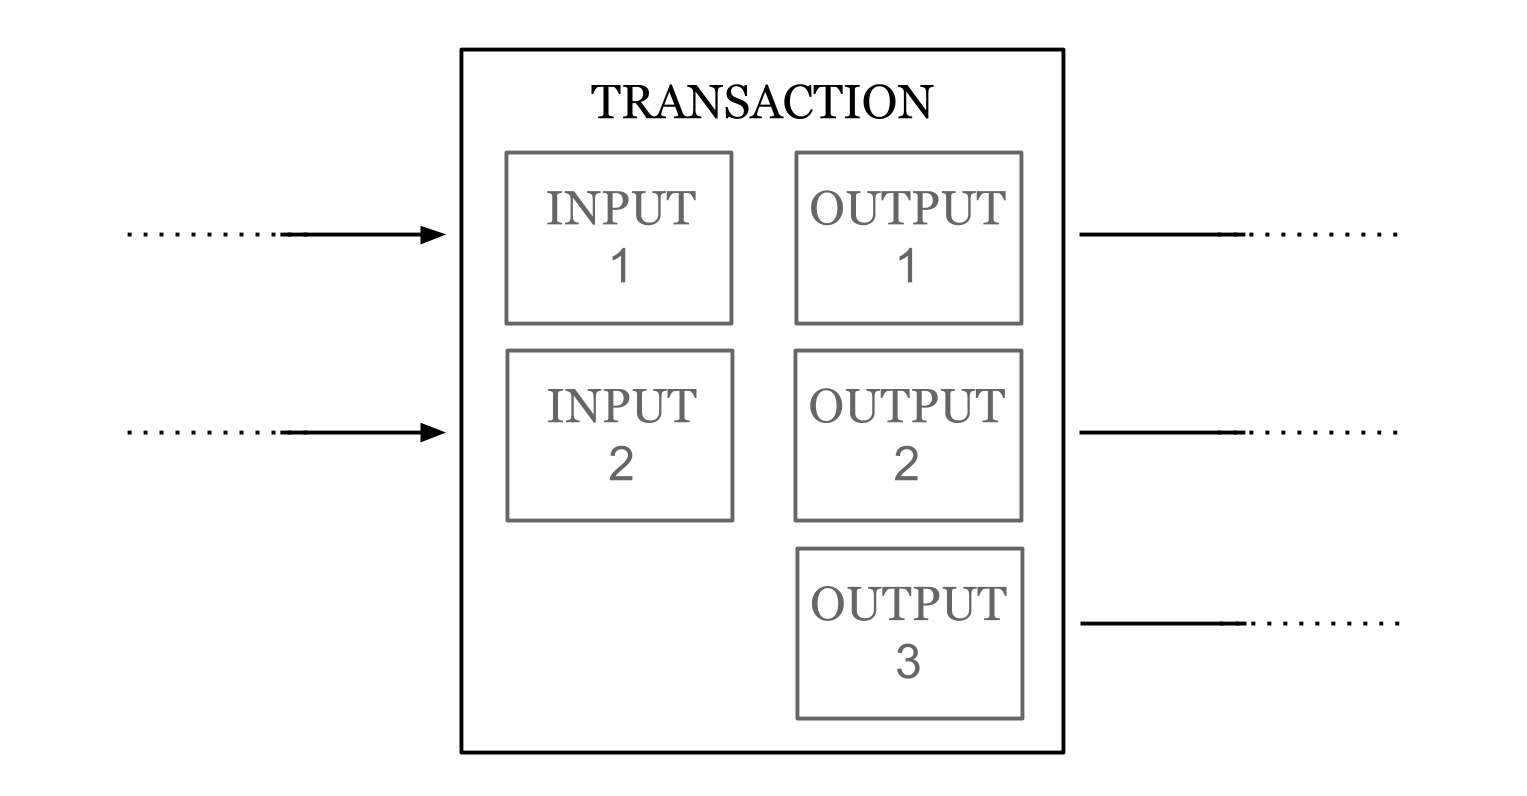
\includegraphics[width=0.75\linewidth]{Images/Diagrams/blockchain_many_inputs_outputs.png}
    \caption{Each transaction in a cryptocurrency contains one or many inputs and one or many outputs (with the exception of ``Coinbase'' transactions where new coins are created).}
    \label{fig:bitcoin_many_in_out}
\end{figure}

\paragraph{Witness Data}
Witness Data was first introduced to Bitcoin in 2015 with SegWit\cite{bitcoin_segwit}. It allows 'thin' clients to verify transactions without possessing a large proportion of the blockchain whilst fixing transaction malleability problems. This might seem like it would be especially useful for my project since the issue of client storage/computing resource management is very important. However, the method that SegWit uses to verify transactions is specific to cryptocurrencies and is therefore not exactly applicable. For example, Bitcoin's transactions contain a list of past transactions as inputs that are a by-product of dealing with money (as mentioned above). Validation is much easier for a messaging platform since a simple signature (and potentially a proof-of-work) is enough to verify the authenticity and validity of a message.
\begin{figure}[ht]
    \centering
    
\includegraphics[width=0.65\linewidth]{Images/Segwit.png}
    \caption{Bitcoin's SegWit has allowed for new innovations in the Bitcoin network such as the \textit{Lightning Network}\cite{bitcoin_lightning_network} whilst maintaining backward compatibility.}
    \label{fig:segwit}
\end{figure}
\newpage

Having stripped the above features from the structure of a transaction, I now have a simplified model:
\begin{table}[H]
\centering
\begin{tabular}{|l|p{8.5cm}|}
\hline
\rowcolor{tblgrey}
Field & Description \\ \hline
version     & Transaction data format version.                          \\ \hline
tx\_from    & Address of sender.                    \\ \hline
tx\_to      & Address of recipient.                                     \\ \hline
lock\_time  & The block number at which this transaction is unlocked. \\ \hline
\end{tabular}
\end{table}

\paragraph{Enabling Group Chats}
To allow for group chats, I needed a way to distribute messages to many people. One solution for this would be to have the sender send a separate message to each member of the group (One to Many). However, this is obviously a bad idea as it will require $n$ transactions for the same message.

Another solution fixes this problem by having a distributed private key for the group (ie. the group has its own address and every user in the group possesses the private  and public keys; One to One). This means that when a user wants to join a new group chat, they do not have to be added to everyone's individual table of recipients. Bitmessage uses a One to One system with a similar structure.

\newpage

\textbf{One to Many}
\textit{ - Advantages}
\begin{itemize}
    \item Everyone knows exactly who is in the group.
    \item Messages can be sent to the group but exclude selected people (effectively allowing users to ``kick'' others from a group).
\end{itemize}

\textit{ - Disadvantages}
\begin{itemize}
    \item Pollutes network and blockchain with the same repeated message. (Alternative is to complicate messages with multiple outputs)
    \item Computationally intensive to generate proof of work for every transaction.
    \item Database of users in group has to be propagated through all users in the group every time someone wants to join.
\end{itemize}


\textbf{One to One}
\textit{ - Advantages}
\begin{itemize}
    \item One transaction per message. (maintaining network and blockchain health)
    \item New users can be added easily.
    \item Tried and tested by Bitmessage. Strong solution.
    \item Doubles as a broadcast channel system for subscription-style update-feed. (Bitmessage ``chans'')
\end{itemize}

\textit{ - Disadvantages}
\begin{itemize}
    \item If someone has access to the private key, then they can eavesdrop on conversations without being known about. (applies to normal message conversations anyway)
    \item Transactions require some extra `post-processing' from clients. (treat as group chat instead of two-user conversations)
\end{itemize}

From the above information, it should be clear to see that the best solution is One-to-One. Therefore this is the solution which I will carry forward.

With this system, if a user wants to create a group chat, they simply create a new key pair. They then distribute the key pair carefully to all those who they wish to add. When a user wants to send a message to the group chat, they will encrypt with their own private key and send a message to the group chat's public key (address). Then, to view the message, all other users will use the group chat's private key. This does mean that if the group chat's public key were to be `leaked', then anyone would be able to send a message into the group chat though they would be unable to read any messages.
\newpage

\paragraph{Lock Time}
Lock time is a feature of Bitcoin transactions that allows for a client to specify when a given transaction should be added to the blockchain. Most of the time, the lock time is unimportant for Bitcoin since, most of the time, clients want their transactions to `go through' straight away. It is useful for investments and binding contracts `to lock' up bitcoins for a period of months or even years.

It's easy to see how a feature like this could be useful for a messaging platform. The ability to postpone the sending of a message for a period of time is desirable for many applications. For example, it can be used as a `reminders' system allowing users to send messages to themselves at a later date. All that is required is that the user has a connection to the platform's network when they first announce the message to be sent. 

This is also easy to achieve from a design perspective since a restriction can be placed on blocks to force `miners' (clients who try to create blocks) to only accept blocks where all included transactions have a lock time that has since ended. Any transaction that is still locked is not to be added to a new block or the entire block will be deemed invalid and rejected.

Whilst this feature does add unnecessary complexity, I believe that it will improve the appeal and utility of the platform enough to be worth including. The extra complexity is mostly implementation detail anyway. This is already included in my model of a transaction with the field \textbf{lock\_time}.

\paragraph{Stickers and Message Types}
If I want to allow for the functionality of a modern messaging service, then I will need to have different kinds of messages. For example, if I want `stickers' to be available, then it would make sense to have that as a message-type. I have compiled all the message types I want into the following table:
\begin{table}[H]
\centering
\begin{tabular}{|p{3cm}|p{8.5cm}|}
\hline
\rowcolor{tblgrey} 
Message type    & Description                                                                               \\ \hline
text            & Simple message in text. (default)                                                         \\ \hline
acknowledgement & A message that contains no actual content, only to indicate that a message has been read. \\ \hline
sticker         & Contains a type of sticker and a position for it in the chat.                                        \\ \hline
reaction        & Similar to Acknowledgement but contains either a Unicode character (emoji) as a reaction or a text reply. \\ \hline
file            & Similar to text but is binary file contents instead of plain text.                       \\ \hline
\end{tabular}
\end{table}

Through the above list of message-types, users should be able to communicate effectively and expressively in a similar manner to that of Facebook Messenger or Whatsapp. For each of these message types, I have decided the fields to be set.

If a user chooses to create a simple `\textbf{text}' message, then the following fields should be set.
\begin{table}[H]
\centering
\begin{tabular}{|p{2.5cm}|p{8.5cm}|}
\hline
\rowcolor{tblgrey} 
Field           & Description                                               \\ \hline
encoding        & Encoding standard for decoding bytes to text. (eg. \texttt{UTF-8}) \\ \hline
data            & Simple plain-text message.                                \\ \hline
\end{tabular}
\end{table}

If a user chooses to create an `\textbf{acknowledgment}' message, then the following field should be set.
\begin{table}[H]
\centering
\begin{tabular}{|p{2.5cm}|p{8.5cm}|}
\hline
\rowcolor{tblgrey} 
Field           & Description                                               \\ \hline
rmsg\_id         & The msg\_id of the message which is being acknowledged.   \\ \hline
\end{tabular}
\end{table}

If a user chooses to create a `\textbf{sticker}' message, then the following fields should be set.
\begin{table}[H]
\centering
\begin{tabular}{|p{2.5cm}|p{8.5cm}|}
\hline
\rowcolor{tblgrey} 
Field           & Description                                               \\ \hline
sticker\_pack   & The sticker pack which contains the chosen sticker.       \\ \hline
sticker\_index  & The index of the chosen sticker in its sticker pack.      \\ \hline
\end{tabular}
\end{table}

If a user chooses to create a `\textbf{reaction}' message, then the following fields should be set.
\begin{table}[H]
\centering
\begin{tabular}{|p{2.5cm}|p{8.5cm}|}
\hline
\rowcolor{tblgrey} 
Field           & Description                                               \\ \hline
rmsg\_id         & The message to be responded to.                           \\ \hline
encoding        & Encoding standard for decoding bytes to text.      \\ \hline
data            & Plain-text message data (could be single Unicode character or string reply).      \\ \hline
\end{tabular}
\end{table}

If a user chooses to create a `\textbf{file}' message, then the following fields should be set.
\begin{table}[H]
\centering
\begin{tabular}{|p{2.5cm}|p{8.5cm}|}
\hline
\rowcolor{tblgrey} 
Field           & Description                                               \\ \hline
file\_name      & Name of file.                                             \\ \hline
file\_type      & Type of file (eg. PDF, PNG, JPEG).                        \\ \hline
data            & Binary file data.                                         \\ \hline
\end{tabular}
\end{table}

You will notice that a new field now has to be introduced to msg in order for \textbf{acknowledgments} and \textbf{reactions} to work. I call this the \textbf{msg\_id} and this provides a way of referencing a previous message. This id is specific to each chat and also provides a way of reducing the possibility of duplicate messages entering a chat.

Now that I have a new field, I will add that to the list of tx fields. Now a transaction looks as follows. Here I also add in the fields for message type and message data.
\begin{table}[H]
\centering
\begin{tabular}{|p{2.5cm}|p{8.5cm}|}
\hline
\rowcolor{tblgrey}
Field & Description\\ \hline
version     & Transaction data format version.                              \\ \hline
lock\_time  & The block number at which this transaction is unlocked. \\ \hline
tx\_from    & Address of sender.                        \\ \hline
tx\_to      & Address of recipient.                                         \\ \hline
msg\_id     & msg\_id of message. (used for acknowledgements and reactions) \\ \hline
msg\_type   & Type of message. (text, acknowledgment, sticker...)          \\ \hline
msg         & Message object. (has different subfields depending on msg\_type, as above) \\ \hline
\end{tabular}
\end{table}

\newpage
\label{para:bf}
\paragraph{Bloom Filters}
A good way of improving search efficiency in the blockchain would be to implement Bloom filters. Bloom filters give an indication as to whether or not a particular item is in a data set. They are probabilistic data structures meaning that they indicate either that an item \textit{may} be in a set or that it is \textit{definitely not} in a set. This is obviously very helpful as it would mean far fewer blocks would have to be transmitted through the network and clients would no longer have to intensively search through every single block when searching for any incoming messages.
\begin{figure}[h]
    \centering
    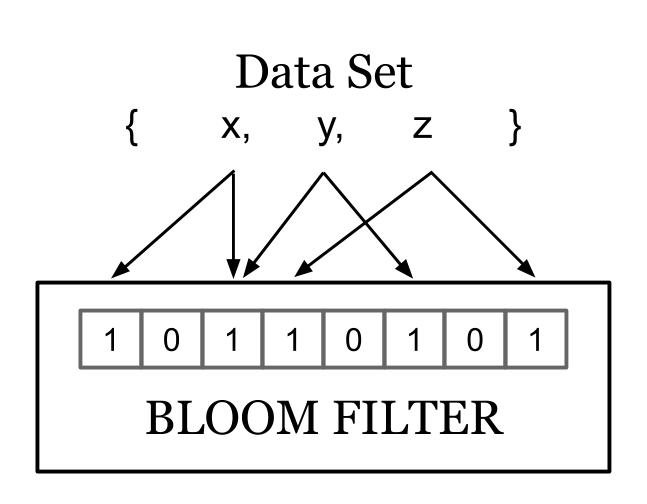
\includegraphics[width=0.5\linewidth]{Images/Diagrams/bloom_filters.png}
    \caption{Bloom filters use multiple hash functions (here just 2) to set the bits in an array. Items can be checked by hashing them and reading the contents of the array at the corresponding indices.}
    \label{fig:bfs}
\end{figure}

Bloom filters may seem very useful but, for them to be applicable to this project, I will have to include some form of identifier on each transaction. In the case of Bitcoin, the Bloom filter can simply use the addresses of the outputs to transactions. However, if I want the platform to retain more anonymity, then I will have to store something else.
This led to the development of what I call the chat identifier or \textbf{ChatID}. The ChatID is attached (unencrypted) to messages that run between users of a chat. This ChatID is decided when the two parties first make contact and maintained for the duration of the chat or until all parties unanimously agree to change it. Group chats have a single ChatID and behave identically to any other chat. Bloom filters can then be created by `full nodes' (those nodes who provide more services to the network).

With this development, clients can now more quickly and efficiently search the blockchain for messages that are intended for them.

However, to make the idea of a ChatID more effective, it would be useful to be able to calculate the ChatID for a chat. In the future, this would mean using the keys of the sender and receiver to generate the ChatID. However, this introduces the problem of needing a shared secret and risks defeating the point of ChatID entirely. For now, I am using the following formula to calculate a ChatID.

\[ \textit{ChatID} = H(H(\textit{R})) \]
where
\[
    \begin{cases}
        H \coloneqq \textrm{SHA256 hash function} \\[6pt]
        R \coloneqq \textrm{Cryptographically secure random large number} \\[6pt]
    \end{cases}
\]

Using what is effectively a random number as a ChatID means that users will need to exchange a ChatID in order to create a chat. This problem could be effectively removed by exchanging a ChatID every time an address is exchanged.

It's also worth noting that anyone can use any ChatID; by definition, there is no way of verifying that a ChatID belongs to a specific group. If a user does use the ChatID of an existing chat then the original users of the chat will simply be unable to decrypt it and can ignore it.

\paragraph{Message Encryption}
To actually protect the content of messages and their respective senders and receivers, some form of encryption is necessary. The easiest method for protecting message content is to use encryption on only the message content and not on the addresses of the sender and receiver. This has the advantage of avoiding the need for a ChatID system as mentioned in paragraph \href{para:bf}{Bloom Filters} but this would obviously go against my aims for true anonymity. Using this method would result in so-called `pseudonymity', where the users' true identities cannot be linked to their address easily except for when a malicious user analyses and cross-references their messages. As discussed in the research phase of this project, I do not believe that `pseudonymity' is sufficient to protect users' privacy and thus I can and will not use this method.

The advent of the ChatID idea allows for a more elegant approach in which the whole transaction is encrypted (except for some metadata and the ChatID of course). This means that only the sender and receiver can see the addresses of their counterparts and not just anyone. This solution seems to me to be very effective at achieving the goals of this project and is `tried and tested' by Bitmessage as they use a similar method with some modifications (ie. no ChatID). I like the idea of this system because it makes every transaction completely unintelligible for an anyone who isn't part of the chat. Another key decision here is how to make this system work for group chats. I have already come to the conclusion that the `one-to-one' method is the way forward and therefore it makes sense for there to be only one ChatID for a group chat.

However, it is clear that some of a transaction's data must remain unencrypted. I have decided that the `version' field must remain unencrypted since the version of the platform may determine how the encrypted data is to be decrypted. It is also important because it allows clients to disclude messages with older versions from their block generation (older versions may contain insecure encryption techniques). This means that in the future, the algorithm for encryption and decryption of transactions could be changed.

Now I must decide which fields should be encrypted and which shouldn't be. Obviously the message data must be encrypted. So too must the addresses of the sender and receiver in order to preserve anonymity as discussed above. I have also concluded that some fields should not be encrypted such as the version field.

The following table shows the fields of a transaction which I believe ought to be encrypted.
\begin{table}[H]
\centering
\begin{tabular}{|p{2.5cm}|p{8.5cm}|}
\hline
\rowcolor{tblgrey}
Field & Description\\ \hline
msg\_id     & msg\_id of message. (Used for acknowledgements and reactions)\\ \hline
tx\_from    & Address of sender.                       \\ \hline
tx\_to      & Address of recipient.                                        \\ \hline
msg\_type   & Type of message. (text, acknowledgment, sticker...)          \\ \hline
msg         & Message object. (has different subfields depending on msg\_type) \\ \hline
\end{tabular}
\end{table}

Also important are the curve parameters for encryption. I have decided to use the same curve as Bitcoin (\textit{secp256k1}\cite{secp256k1})\footnote{As well as choosing, the same curve, I am choosing the same subgroup, prime-field etc.}. There are two reasons for this. The first is that it has been `tried and tested'. In other words, if the curve were to be majorly, cryptographically flawed in some way, then there is a high probability that these flaws would have been discovered by now and would have led to the cryptocurrency's demise. Bitcoin chose the \textit{secp256k1} curve for many reasons and it doesn't make sense to redo the time-consuming work of finding and checking a curve. The other reason is that the curve is relatively well understood in the sense that the calculations for encryption, decryption, signing and so on are all well defined and optimised. It is very possible that, in the future, a `backdoor' into the \textit{secp256k1} curve will be found. If that is the case, then an update would have to be deployed to change the platform's curve\footnote{For simplicity, I am choosing not to include curve definition and parameters in each tx (ie. Not defining $a$, $b$ for any given curve, $y=x^3+ax+b$). Therefore the curve parameters are fixed unless the entire platform is updated.}.

\subparagraph{Addresses vs Public Keys}\label{subpara:addrsvspubkeys}
Addresses are also key to the function of the Bitcoin infrastructure. Bitcoin separates public keys from addresses\footnote{A wallet address is calculated by hashing the public key ( $H(H(\textit{public\_key}))$ ).}. There are some good reasons for this. It serves as a last line of defense in case the Bitcoin curve is `backdoored'. For the purposes of this project, the separation of public keys and addresses is not only non-essential but overly-complicated in my opinion. Otherwise, a public key retrieval system similar to Bitcoin's would have to be designed.

\subparagraph{ECIES}
As in Bitmessage\cite{bitmessage_ecies}, the encryption scheme I have chosen to use is the ``Elliptic Curve Integrated Encryption Scheme''. This requires the following pieces of data in order to allow for an encrypted payload to be decrypted.
\begin{table}[H]
\centering
\begin{tabular}{|p{1.5cm}|p{8.5cm}|}
\hline
\rowcolor{tblgrey}
Name        & Comments              \\ \hline
iv          & Initialization Vector used for AES-256-CBC.   \\ \hline
x           & $x$ component of ephemeral public key $R$.    \\ \hline
y           & $y$ component of ephemeral public key $R$.    \\ \hline
mac         & Message authentication code.                  \\ \hline
\end{tabular}
\end{table}

\hspace{-\parindent}The steps to \textbf{encrypt} are as follows (identical to Bitmessage\cite{bitmessage_ecies}):
\begin{enumerate}
    \item The destination public key is called $K$.
    \item Generate 16 random bytes using a cryptographically secure random number generator. Call them \textit{iv}.
    \item Generate a new random EC key pair with private key called $r$ and public key called $R$.
    \item Do an EC point multiply with public key $K$ and private key $r$. This gives you public key $P$.
    \item Use the $x$ component of public key $P$ and calculate the \textbf{SHA512} hash $H$.
    \item The first 32 bytes of $H$ are called \textit{key\_e} and the last 32 bytes are called \textit{key\_m}.
    \item Pad the input text\footnote{This just refers to the input payload (ie. the fields that will later become \textit{encrypted\_payload}) in bytes.} to a multiple of 16 bytes, in accordance to PKCS7\cite{pkcs7}.
    \item Encrypt the data with \textbf{AES-256-CBC}, using \textit{iv} as initialization vector, \textit{key\_e} as encryption key and the padded input text as payload. Call the output \textit{cipher\_text}.
    \item Calculate a 32 byte MAC with \textbf{HMACSHA256}, using \textit{key\_m} as salt and \textit{iv} + $R$ + \textit{cipher\_text} as data. Call the output \textit{mac}.
\end{enumerate}
Thus the steps to \textbf{decrypt} are as follows (again identical to Bitmessage):
\begin{enumerate}
    \item The private key used to decrypt is called $k$.
    \item Do an EC point multiply with private key $k$ and public key $R$. This gives you public key $P$.
    \item Use the $x$ component of public key $P$ and calculate the \textbf{SHA512} hash $H$.
    \item The first 32 bytes of $H$ are called \textit{key\_e} and the last 32 bytes are called \textit{key\_m}.
    \item Calculate MAC' with \textbf{HMACSHA256}, using \textit{key\_m} as salt and \textit{iv} + $R$ + \textit{cipher\_text} as data.
    \item Compare MAC with MAC'. If not equal, decryption will fail.
    \item Decrypt the cipher text with \textbf{AES-256-CBC}, using \textit{iv} as initialization vector, \textit{key\_e} as decryption key and the \textit{cipher\_text} as payload. The output is the padded input text.
\end{enumerate}

I can now add these fields to the structure of a tx. This gives the following.
\begin{table}[H]
\centering
\begin{tabular}{|p{3cm}|p{8.5cm}|}
\hline
\rowcolor{tblgrey}
Field       & Description\\ \hline
version     & Transaction data format version.                          \\ \hline
chat\_id    & ChatID of chat.   \\ \hline
lock\_time  & The block number at which this transaction is unlocked. \\ \hline
iv          & Initialisation vector used for AES-256-CBC.   \\ \hline
x           & $x$ component of ephemeral public key $R$.    \\ \hline
y           & $y$ component of ephemeral public key $R$.    \\ \hline
mac         & Message authentication code.                  \\ \hline
encrypted\_payload & Encrypted payload.                     \\ \hline
\end{tabular}
\end{table}


\paragraph{Proof of Work}
Proof-of-work is at the heart of most cryptocurrency and blockchain projects. It is an indirect way of ensuring the security of a blockchain. Normally it takes the form of a \textit{nonce}. A \textit{nonce} is usually a number stored in the block headers. Blocks are only deemed valid if their \textit{nonce} results in a Merkle hash that satisfies a certain difficulty.

Traditionally, proof-of-work is calculated by hashing the entire block using Merkle root hashes and then comparing the resulting hash to a \textit{target} value. If the resulting hash is lower than the difficulty value, then the block is valid. This means that the difficulty can be changed to predictably change the block-time.

Proof-of-Work is not just applicable to blocks however, it is also used by Bitmessage on individual messages in order to discourage \textit{denial-of-service}\cite{bitmessage_pow} attacks where a user might try to rapidly send a large quantity of messages in an attempt to slow down or even halt the platform. This is a feature that I want to implement as DoS attacks could become a major problem.

The Bitmessage proof-of-work target value for individual messages is calculated as follows:

\begin{center}
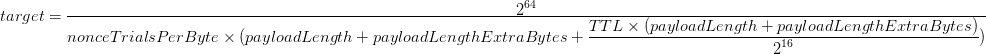
\includegraphics[width=\linewidth]{Images/Diagrams/bitmessage_pow.png}
\end{center}

This is obviously quite a large formula and relies on several variables not discussed up to this point. It uses some variables which are less relevant to the design of \textit{my} platform.

To begin with, I stripped the formula of unwanted variables such as TTL (Time-To-Live for the given message) to give a simpler formula from which to build on. This resulted in the following:
\begin{center}
\[\textit{target} = \dfrac{2^{64}}{\textit{payloadLength} + \dfrac{\textit{payloadLength}}{2^{16}}}\]
\end{center}

As the \textit{payloadLength}\footnote{The \textit{payloadLength} refers to the number of bytes that make up the transaction.} increases, the \textit{target} will decrease. However, with this system, the target will be too easy for small messages. This is why Bitmessage utilises message padding in the form of \textit{payloadExtraBytes}. \textit{payloadExtraBytes} is set to 1000\footnote{It should be noted that the value of \textit{payloadExtraBytes} can be tuned to change the difficulty of sending a message. }. With \textit{payloadExtraBytes} reintroduced, the formula reads:
\begin{center}
\[\textit{target} = \dfrac{2^{64}}{\textit{payloadLength} + \textit{payloadExtraBytes}  + \dfrac{\textit{payloadLength} + \textit{payloadExtraBytes}}{2^{16}}}\]
\end{center}

Unlike PoW for blocks, the target value for message transactions is not dynamically changed in Bitmessage. This means that, unless the entire protocol is updated, the difficulty value is effectively static for any given messages of the same length. I don't think that this will be realistically sustainable because if the platform were to gain real popularity in the future, then the growth in processor speed might render the DoS protection futile.

I would like the difficulty of creating a transaction to be dynamically changed to reflect the growth in computational power. To do this I need a variable that will change over time. For example, I could use the block-difficulty constant as that would grow over time with the growth of popularity and computational power. However, this example would introduce a new problem; the transaction creator would have to know in which block their transaction is to be contained ahead of time which is simply impossible. I am not sure if there is an effective solution for this but, for now, I am basically going to stick with the above formula. We can simplify\footnote{The reason why it is ok to remove the second part of the denominator is because that was just a way of scaling Bitmessage's PoW difficulty with TTL (Time-To-Live). Since there is no such thing as TTL for a transaction on my platform, this can be ignored.} this further to the following.
\vspace{-0.5cm}
\begin{center}
\[\textit{target} = \dfrac{2^{64}}{\textit{payloadLength} + \textit{payloadExtraBytes}}\]
\end{center}

In the future, I hope to modify this formula to be more dynamic as discussed.

To actually calculate a PoW, a client should use the following formula (very similar to Bitmessage):


Repeat until \textit{result} $<$ \textit{target}:
\[
    \textit{result} = H(H(\textit{nonce} + \textit{encrypted\_payload})) \\
\]
where
\[
    \begin{cases}
        H \coloneqq \textrm{SHA256 Hash function} \\[6pt]
        + \coloneqq \textrm{concatenation} \\[6pt]
        \textit{nonce} \coloneqq \textrm{randomly chosen number incremented until \textit{result} is valid}
    \end{cases}
\]

Finally, I now have to add these variables to the structure of a transaction. This gives the following.
\begin{table}[H]
\centering
\begin{tabular}{|p{3cm}|p{8.5cm}|}
\hline
\rowcolor{tblgrey}
Field       & Description\\ \hline
version     & Transaction data format version.                          \\ \hline
chat\_id    & ChatID of chat. \\ \hline
tx\_id      & PoW value for tx. $H(H($\textit{nonce + encrypted\_payload}$))$ \\ \hline
lock\_time  & The block number at which this transaction is unlocked. \\ \hline
nonce       & PoW nonce value. \\ \hline
iv          & Initialisation vector used for AES-256-CBC.   \\ \hline
x           & $x$ component of ephemeral public key $R$.    \\ \hline
y           & $y$ component of ephemeral public key $R$.    \\ \hline
mac         & Message authentication code.                  \\ \hline
encrypted\_payload & Encrypted payload. \\ \hline
\end{tabular}
\end{table}

This structure for a transaction now contains all the fields which I believe are necessary for this platform. This is the finished design for \textit{v1}. However in \textit{v2}, I will look to find areas which can be improved.

\subsubsection{Blocks}
Blocks are fundamental to this project in that they are what separate this platform from other services like Bitmessage. The concept of a blockchain is inherently based around the grouping of transactions (in the case of a cryptocurrency) into blocks. The block is what differentiates a blockchain from a basic database and the block's proof-of-work is the backbone of trustless interaction between users of a blockchain.

The block is a relatively simple structure. It contains a section for headers which store all the metadata and a section for transactions. The headers include information such as the version of the platform that the block was created with; the number of included transactions; the proof-of-work nonce; and more. To begin with, I will start with a stripped model. From there, I will build up the design progressively.
\begin{table}[h]
\centering
\begin{tabular}{|l|l|}
\hline
\rowcolor{tblgrey} 
Header      & Description                                       \\ \hline
version     & Version of platform used by block creator.        \\ \hline
no          & Block number.                                     \\ \hline
\end{tabular}
\end{table}

The block number of a block is defined as 0 for the first block, 1 for the second, 2 for the third and so on. It is used by the \textit{lock\_time} field in a transaction.

I need to create a blockchain which means that I require a way of identifying a block and linking it to a previous block. I will accomplish this with Merkle root hashes.

\paragraph{Merkle Root Hashes}
Merkle root hashes are a way of hashing a large array of data such as a list of transactions. It does this by hashing neighbouring elements together, then concatenating neighbouring hashes together and hashing those. This is repeated over and over until only one hash is left (see \autoref{fig:merklert}).
\begin{figure}[h]
    \centering
    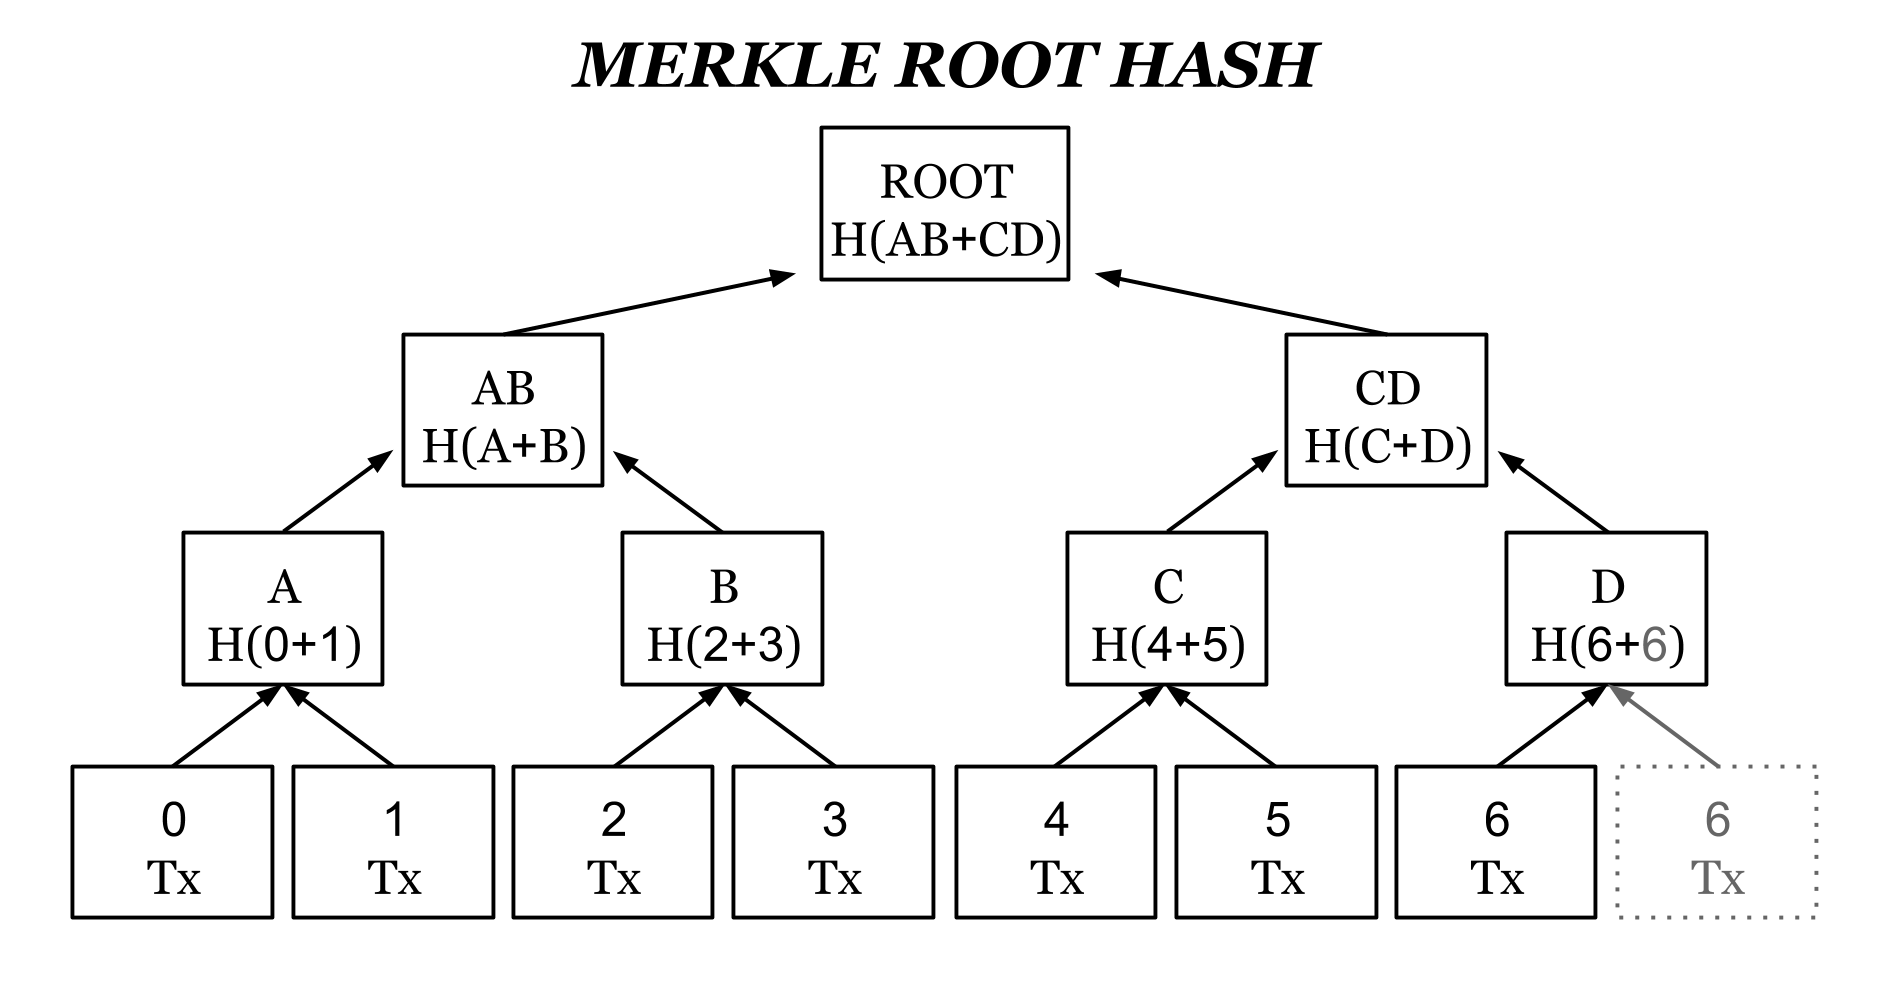
\includegraphics[width=0.95\linewidth]{Images/Diagrams/merkle_root.png}
    \caption{Merkle root hashes are calculated by recursively hashing transactions and then hashes of transactions and then hashes of hashes and so on...}
    \label{fig:merklert}
\end{figure}

Merkle hashes provide a good way of identifying blocks as they cannot be forged. It is also extremely unlikely to ever have a collision between two blocks' roots. This is ideal for identifying blocks and so I will be using this as the `BlockID'.

\[\textit{block\_id} = H(M(\textit{transactions}))\]
where
\[\begin{cases}
        H \coloneqq \textrm{SHA256 Hash function} \\[6pt]
        M \coloneqq \textrm{Merkle Root Hash function. (using SHA256)}
\end{cases}\]

\vspace{10pt}

This can then be added to the design of a block as follows.
\begin{table}[H]
\centering
\begin{tabular}{|p{2.5cm}|p{8.5cm}|}
\hline
\rowcolor{tblgrey} 
Field      & Description                                         \\ \hline
version    & Version of platform used by block creator.          \\ \hline
no         & Block Number.                                       \\ \hline
block\_id  & The Merkle root hash of the current block.          \\ \hline
prev       & The BlockID the previous block in the blockchain.   \\ \hline
tx\_l       & A list of transactions.                            \\ \hline
\end{tabular}
\end{table}

Notice that I have also added the \textbf{prev} field. This references the BlockID of the previous block, thus creating a blockchain.

\begin{figure}[h]
    \centering
    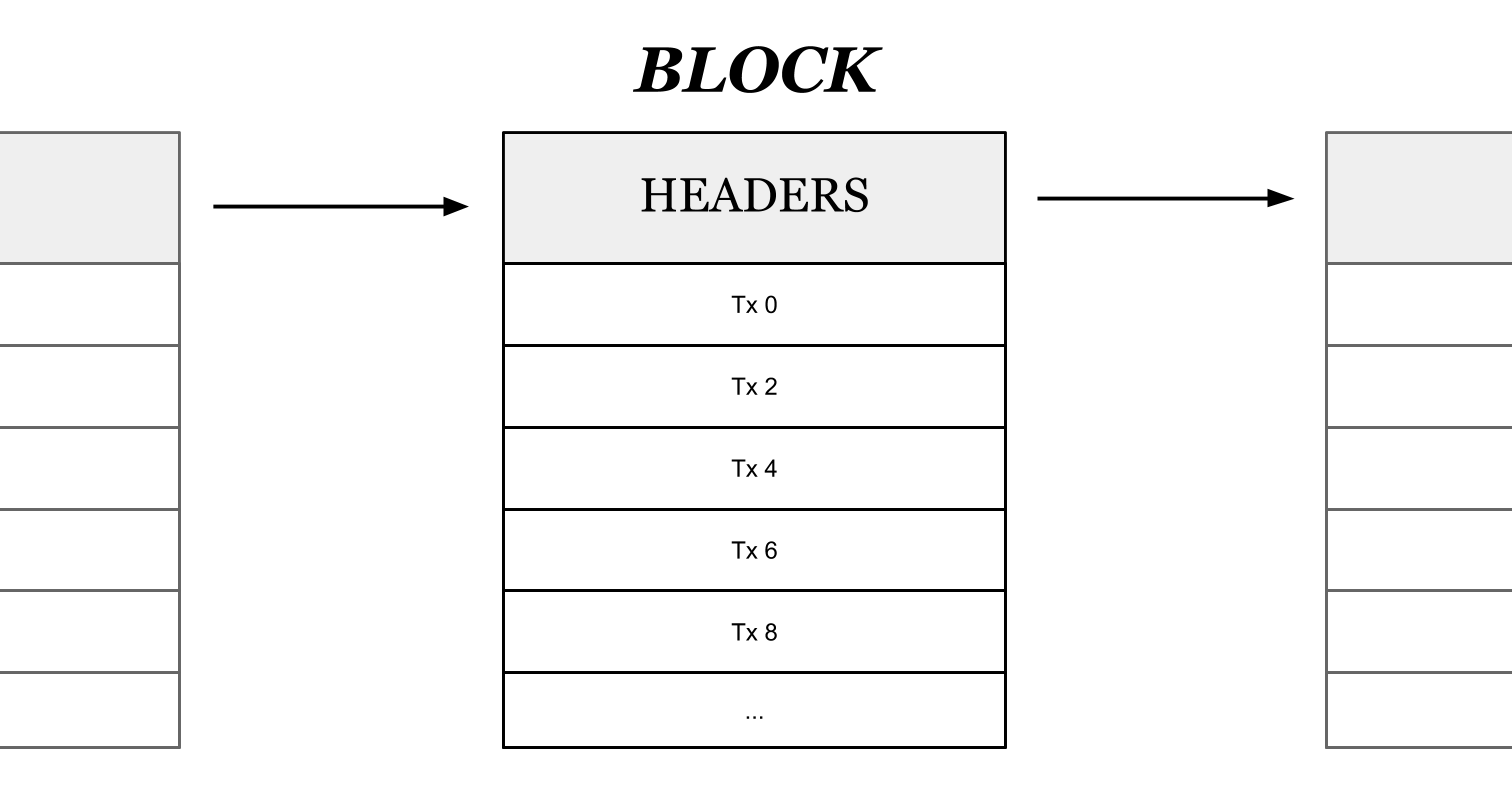
\includegraphics[width=\linewidth]{Images/Diagrams/blockchain_block.png}
    \caption{A simplified diagram of the structure of a block.}
    \label{fig:block}
\end{figure}

\paragraph{Proof of Work}
Proof of work for blocks will be similar to the proof of work for transactions with a few key differences. First of all, the process of generating a proof of work will need to change. Instead of hashing a \textit{nonce} and \textit{encrypted\_payload}, we will be hashing the list of transactions (Merkle root) with a new nonce.

This will change the process of creating a BlockID from the previous \[H(M(\textit{transactions}))\] to the new \[H(\textit{nonce} + \textit{prev} +  M(\textit{transactions}))\] much like the \textit{tx\_id} of a transaction.

I think that the difficulty value should be computed, as in Ethereum, with the following formula where \textit{block\_time} is the time between creation of the two most recent blocks.
\[\textit{difficulty}_{\textit{new}} = \textit{difficulty}_{\textit{old}}
\ + \ \left\lfloor\dfrac{\textit{difficulty}_{\textit{old}}}{2048}\right\rfloor \times \max\left(1- \left\lfloor \frac{\textit{block\_time}}{10} \right\rfloor,\ -99\right)\]
The reason I chose this equation is because it has been `tried and tested' by the Ethereum platform and was designed by experts and professionals in the field of cryptography. It makes sense to not rework crucial elements of the platform for no reason.

The target hash value can then be calculated as follows.
\[\textit{target}_{\textit{new}} = \frac{\textit{target}_{\textit{old}}} {\textit{difficulty}_{\textit{new}}}\]

A block is only valid if the nonce results in a BlockID which is less than the current difficulty value. I can now add the required fields to the structure of a block.
\begin{table}[H]
\centering
\begin{tabular}{|p{2.5cm}|p{8.5cm}|}
\hline
\rowcolor{tblgrey} 
Field      & Description                                         \\ \hline
version    & Version of platform used by block creator.          \\ \hline
no         & Block Number.                                       \\ \hline
block\_id  & The Merkle root hash of the current block. (used for PoW)  \\ \hline
prev       & The BlockID of the previous block in the blockchain.   \\ \hline
nonce      & PoW nonce value for the block.                      \\ \hline
ts         & Timestamp of block when created.                    \\ \hline
tx\_l       & A list of transactions.                            \\ \hline
\end{tabular}
\end{table}

Note that a block timestamp (\textit{ts}) is needed to calculate block time which is essential for the function of proof of work.

\paragraph{Bloom Filters}
With the introduction of the ChatID on transactions, I can begin to implement a bloom filter into the structure of the platform. The bloom filter itself requires two or more hash functions\footnote{To circumvent the need for more than two hash functions, it is actually possible to derive subsequent hash functions from two originals in the form $h3(x) = h1(x) + i \times h2(x)$ (this is well documented and tested here\cite{harvard_better_bloom_filters}).} which are independent and uniformly distributed. Unfortunately, bloom filters need to be very large to be practically useful. A useful bloom filter would be on the order of KiloBytes for this application and therefore cannot be included in block headers. Instead they will have to be provided by full nodes as a network service (this will be discussed in the network protocol design).

The actual parameters for a bloom filter need not be standardised since every client will implement it differently, and potentially parameters could be optimised for each block.

\paragraph{Uncle Blocks}
Since Bitcoin has such a long block time (10 minutes), it does not require the use of uncle blocks or GHOST protocol in order to maintain the security of the platform. However, Ethereum's 10--20 second block times \textit{do} mean that the platform requires some countermeasures (see \textbf{\autoref{para:ghostprotocol}}). Whilst the block times of this platform share the 10--20 second duration, the platform itself is very different. There is no currency being exchanged or created and thus there is no reward for the creator of a block. Since the incentive for creating a block no longer exists, it is reasonable to assume that efforts to overpower the network (51\% attack) will be less common and aggressive. However, there is always the possibility of a `51\% attack' and if that were to happen, then the controlling node would be able to deliberately omit transactions of their choosing or alternatively even block all transactions from being added to the chain. It's easy to see how this could become frustrating for a user of the platform as none of their messages would make it to their destination. However, critically, there is no loss of anonymity in terms of the identity of the senders and receivers of messages.

To be clear, I have opted to ignore the GHOST protocol and instead follow Bitcoin, where the longest chain is considered truth and no `uncle blocks' are taken into consideration in the creation of a block. I am essentially relying on the resolve of individual network users contributing their computing power towards the cause.

\paragraph{Authors}
If a miner wants to claim the discovery of a block, then they can add their main public key to the block with a signature. I think that they should leave a signature so that it is possible to prove the identity of an author. This still allows for full anonymity since a client can create a new set of keys for every new block they create. Signatures should also be mandatory for all blocks since it will make mining slower for those who choose to include them.

To calculate the signature, the client simply signs the block number \textit{no} field with their public key.



The block signature can be calculated as follows:
\[\textit{author\_sig} = S(\textit{no})\]
where
\[S \coloneqq \textrm{Encrypt with private key of author.}\]

With this addition, clients can now know who created a particular block or claim its creation.

\newpage

With all these additions and modifications, the structure of a block now looks like this. This is the finished structure for \textit{v1}.
\begin{table}[H]
\centering
\begin{tabular}{|p{2.5cm}|p{8.5cm}|}
\hline
\rowcolor{tblgrey} 
Field      & Description                                         \\ \hline
version    & Version of platform used by block creator.          \\ \hline
no         & Block Number.                                       \\ \hline
block\_id  & The Merkle root hash of the current block. (used for PoW)  \\ \hline
prev       & The BlockID of the previous block in the blockchain.   \\ \hline
nonce      & PoW nonce value for the block.                      \\ \hline
author\_x  & Author's public key \textit{x} component.           \\ \hline
author\_y  & Author's public key \textit{y} component.           \\ \hline
author\_sig& Block signature.                                    \\ \hline
ts         & Timestamp of block when created.                    \\ \hline
tx\_l      & A list of transactions.                            \\ \hline
\end{tabular}
\end{table}


\newpage
\subsection{Network Protocol \textit{v1}}
This section documents the design process for the proposed network protocol. The network protocol is the `set of rules' to be followed by all devices on the peer-to-peer network and is how different devices know how to interact with each other. This needs to be standardised for a network for obvious reasons.

\subsubsection{Peer to Peer}
Much like the networks of Bitcoin and Bitmessage, the network for this proposed platform is peer-to-peer (p2p) based. This is important for retaining anonymity since there is no centralised entity controlling access to data.

This type of network is explained and discussed more thoroughly in the research section of this project (\autoref{subsubsec:whatisablockchain}).

\subsubsection{Underlying Protocol Layers}
The network protocol that this project builds itself relies upon many lower-level layers of protocols. This abstraction will make network protocol design simpler and reduce the complexity of the design.

The industry standard for network communication is Transmission Control Protocol (TCP) which itself lies on top of the IP protocol. TCP is used for the majority of web communications and is the `backbone' of HTTP. It is well documented and supported by all major programming languages making it ideal for a network such as this. It handles many of the more difficult problems with network interaction such as packet loss and flow control. However it can be slower than other protocols due to it having these features. An alternative to TCP would be User Datagram Protocol (UDP) which is known for being better at low-latency connections than TCP but only if the sender and recipient are more tolerant of packet loss.

\newpage

\textbf{TCP}
\textit{ - Advantages}
\begin{itemize}
    \item Widely used with excellent implementation documentation. This makes for simple design and implementation and a better developer experience overall.
    \item Handles packet loss well. This is useful for this blockchain service because it means that all communications are guaranteed\footnote{In the case where a network client (sender or receiver) is disconnected from the network entirely during communications, the connection stream must be dropped and the packets will never make it to their destination.} to reach their destination.
\end{itemize}

\textit{ - Disadvantages}
\begin{itemize}
    \item Designed for relatively small packets and may not handle large quantities of data very well. When a client sends a block to another client, the network may suffer from slow downs.
    \item Designed with ordering and ease-of-use in mind over speed. This will limit the rate of communications and slow down the network.
\end{itemize}

\textbf{UDP}
\textit{ - Advantages}
\begin{itemize}
    \item All-around faster protocol. Perfect for transfer of fairly large data such as a large list of blocks.
    \item Fewer features means less overhead.
\end{itemize}

\textit{ - Disadvantages}
\begin{itemize}
    \item Harder to implement since doesn't automatically handle features like packet ordering and packet re-sending if any are dropped.
    \item Less well-used by the developer community and therefore often has worse documentation/support.
\end{itemize}

The obvious option here is TCP and from this point onward, that is the option that I will run with. It is worth noting that, in the future, some UDP communications could be implemented into network interactions to speed up specific requests on the network. For example, large transfers of data such as blocks could be modified to make use of UDP or something similar. Also, since it is probable that most implementations of this platform will be open source, it would be fairly easy for a developer to `fork' an implementation and create their own network which makes use of UDP or some other future protocol.

\subsubsection{Network Serialisation}
Serialisation is the way objects get stored on disk and in the network. This decides the order of the fields in a network request and the number of bits assigned to each. This section will inherently overlap somewhat with disk serialisation (ie. the way blocks are stored on disk). However, disk serialisation will be specific to each client implementation. If the network serialisation for the proposed network were to prioritise the wrong fields or be overly `bloated', then the network could become slow and expensive for users, taking up more network bandwidth than necessary. Likewise if the designated field sizes were to be too \textit{small}, then users may have to send more requests than necessary to the network in order to fully communicate or even worse, suffer truncation leading to data loss.

To contain the data, a set of primitive data types must be defined. Here is a set of a few primitives that I know I will need.
\begin{table}[h]
\centering
\begin{tabular}{|l|p{8.5cm}|}
\hline
\rowcolor{tblgrey} 
Data Type  & Description                \\ \hline
uint\_8     & 8 bit integer.            \\ \hline
uint\_16    & 16 bit integer.           \\ \hline
uint\_32    & 32 bit integer.           \\ \hline
uint\_64    & 64 bit integer.           \\ \hline
uint\_128   & 128 bit integer.          \\ \hline
(u)int\_256   & 256 bit (un)signed integer.          \\ \hline
var\_(u)int   & Variably sized, (un)signed integer.    \\ \hline
uint\_xx[\hspace{0.05cm}] & Array of xx-bit integers. (prepended with length) \\ \hline
\end{tabular}
\end{table}

To store integers that are of large sizes, the variably-sized integer \textit{var\_(u)int} consists of two bytes indicating the length in bytes of the following number (followed by the number itself). This will allow for client software to decode very large numbers with no confusion over field sizes that store numbers of variable length. Likewise if the number is small, then no bytes are wasted. Since most of the data that will be used is non-negative, most of these integers are \textbf{unsigned}.

Similarly arrays of integers are prepended with two bytes to indicate the number of elements in them.

\paragraph{Requests} \label{para:requests}
The structure of a request is standard for all requests. This is the lowest level defined by my specification. Bitcoin and Bitmessage have similar network request structures, essentially consisting of the following.
\begin{table}[H]
\centering
\begin{tabular}{|p{2.5cm}|p{2cm}|p{5.5cm}|}
\hline
\rowcolor{tblgrey} 
Data Type   & Field       & Description                                      \\ \hline
uint\_32    & magic       & Magic value indicating origin network.           \\ \hline
uint\_8     & command     & Identifies packet content (ie. encodes the purpose of the message). \\ \hline
uint\_32    & checksum    & Checksum hash of request payload.                \\ \hline
request\_payload & payload     & Actual request payload (ie. content of request). \\ \hline
\end{tabular}
\end{table}

The \textit{checksum} value is an easily-computed value that verifies that the payload is intact. This helps to reduce the possibility of erroneous or potentially incorrect data reaching a client. To calculate the checksum, a node simply computes the SHA256 hash of the request\_payload and takes the first four bytes.

\subparagraph{Magic Value}\label{subpara:magicval}
The \textit{magic} value is a specific number that refers to the network of the request. Bitcoin has a test network that allow for developers to test their software with no real stakes. If the magic value is anything other than 1 of 2 arbitrary values, then the network will reject the request. This is a precaution to avoid cross-protocol confusion.
The process of Bitcoin choosing its magic value is documented briefly in the Bitcoin master code repository\cite{bitcoin_magiccode}.
\begin{minted}{cpp}
    /**
    * The message start string is designed to be unlikely
    * to occur in normal data.
    * The characters are rarely used upper ASCII, not valid as 
    * UTF-8, and produce a large 32-bit integer with any alignment.
    */
\end{minted}
To choose my magic value, I first started with the Bitcoin magic value, $\texttt{D9B4BEF9}_{16}$ (main net), and then I toggled ten random bits.
\begin{align*}
    \textit{Bitcoin\_magic} &= \texttt{11011001101101001011111011111001}_2   \\
    \textit{New\_magic} &= \texttt{11011101111001101010111001001100}_2       \\
                        &= \texttt{DDE6AE4C}_{16}
\end{align*}
This will be the magic value for the main network of my platform.

Similarly for the test network magic, I toggled ten bits of Bitcoin's test net magic value ($\texttt{DAB5BFFA}_{16}$). 
\begin{align*}
    \textit{Bitcoin\_magic}_\textit{test} &= \texttt{11011010101101011011111111111010}_2   \\
    \textit{New\_magic}_\textit{test} &=  \texttt{11001111011100010011101111110011}_2      \\
                        &= \texttt{CF713BF3}_{16}
\end{align*}

It goes without saying that a test network would be present for the default implementation of this platform.

\subparagraph{Commands} The \textit{command} value is, for Bitcoin and Bitmessage, the type of the request being made. For example Bitmessage has several different commands including `version' to indicate a client's protocol version to another device and `inv' to communicate the extent of a client's message inventory. I now have to define which request\_payload types I want (most of these provide similar functionality to Bitcoin's `message types'\cite{bitmessage_messagetypes}\footnote{Note that Bitcoin refers to network requests as `messages'. This is obviously conflicting terminology for a messaging platform and so I will refer to them as \textbf{requests} rather than messages.}).
\begin{table}[H]
\centering
\begin{tabular}{|p{3cm}|p{8cm}|}
\hline
\rowcolor{tblgrey}
Command     & Description\\ \hline
version     & Version of platform being used by node. \\ \hline
verack      & Reply to version.                       \\ \hline
addr        & What other nodes do you know of?        \\ \hline
inv         & How much of the blockchain do you have? \\ \hline
get\_blocks & Give me these blocks.                   \\ \hline
get\_blockheaders & Give me the headers for these blocks. \\ \hline
blocks       & Here are the blocks you asked for.       \\ \hline
blockheaders & Here are the blockheaders you asked for.\\ \hline
check\_blooms   & Check the bloom filters of these blocks for this ChatID.\\ \hline
blooms\_checked & Here are the results of my bloom filter check.          \\ \hline
get\_newtx  & Give me new transactions that haven't been included in a block yet. \\ \hline
newtx       & Here are the transactions you asked for. \\ \hline
\end{tabular}
\end{table}

\begin{center}
    \Large \textit{version}
\end{center}
The \textbf{version} request is how all communications on the network are initiated. Each node sends a `version' request to the other, who returns with a `verack'. A `version' request contains one field indicating the version of the platform being used by the sender node.
\begin{table}[H]
\centering
\begin{tabular}{|p{1.3cm}|p{2.5cm}|p{5.5cm}|}
\hline
\rowcolor{tblgrey}
Data Type   & Field       & Description\\ \hline
uint\_8     & version     & Version of platform being used.                          \\ \hline
uint\_64    & nonce       & Random nonce used to detect connections to self.                   \\ \hline
\end{tabular}
\end{table}

\begin{center}
    \Large \textit{verack}
\end{center}
The \textbf{verack} request is made in response to a `version' request. However, at the start of an interaction between two nodes on the network, both should send `version'. The `verack' request need not contain any fields at all. This means that the \textit{payload} of the request is empty.

\begin{center}
    \Large \textit{addr}
\end{center}
The \textbf{addr} request is made when a node wants to discover new nodes on the network. This is especially important for newer nodes on the network. This request should be made in most interactions between two nodes in order to keep the network online. The `addr' request contains two fields indicating the number of other nodes known and their address.
\begin{table}[H]
\centering
\begin{tabular}{|p{1.5cm}|p{2.5cm}|p{5.5cm}|}
\hline
\rowcolor{tblgrey}
Data Type   & Field       & Description\\ \hline
ip\_addr[\hspace{0.05cm}] & addr\_l       & Array of shared node addresses. (max 1000)                               \\ \hline
\end{tabular}
\end{table}

\begin{center}
    \Large \textit{inv}
\end{center}
The \textbf{inv} request is sent once `verack's have been exchanged. This is so that each node knows which blocks are available to them. They can then close the connection if neither owns a desired block. If a desired block \textit{is} possessed, then the requesting node will send a `get\_blockheaders' or `get\_blocks' request to retrieve it.
\begin{table}[H]
\centering
\begin{tabular}{|p{2.2cm}|p{3cm}|p{5.5cm}|}
\hline
\rowcolor{tblgrey}
Data Type   & Field       & Description\\ \hline
uint\_32[\hspace{0.05cm}] & blocks & List of block numbers of blocks to share.                    \\ \hline
uint\_32[\hspace{0.05cm}] & blockheaders & List of block numbers of block headers to share.                    \\ \hline
uint\_8[\hspace{0.05cm}]  & bloomfilters & List of block numbers for which a bloom filter is possessed.        \\ \hline
\end{tabular}
\end{table}
Note that the blockheader type is identical to the block type except without the \textit{tx\_l} field.

\begin{center}
    \Large \textit{get\_blocks}
\end{center}
The \textbf{get\_blocks} request is sent in order to ask for a given set of blocks. It contains one field: a list of block numbers referring to the requested blocks.
\begin{table}[H]
\centering
\begin{tabular}{|p{2.2cm}|p{3cm}|p{5.5cm}|}
\hline
\rowcolor{tblgrey}
Data Type   & Field       & Description\\ \hline
uint\_32[\hspace{0.05cm}] & block & List of block numbers of blocks wanted.                    \\ \hline
\end{tabular}
\end{table}

\begin{center}
    \Large \textit{get\_blockheaders}
\end{center}
The \textbf{get\_blockheaders} request is sent in order to ask for a given set of blockheaders. It contains one field: a list of block numbers referring to the requested block\_headers.
\begin{table}[H]
\centering
\begin{tabular}{|p{2.2cm}|p{3cm}|p{5.5cm}|}
\hline
\rowcolor{tblgrey}
Data Type   & Field       & Description\\ \hline
uint\_32[\hspace{0.05cm}] & blockheaders & List of block numbers of block headers wanted.                    \\ \hline
\end{tabular}
\end{table}

\begin{center}
    \Large \textit{blocks}
\end{center}
The \textbf{blocks} request is sent in order to return a set of blocks asked for by another node. It contains one field: a list of blocks. If the sender doesn't possess one or more the blocks asked for, then those blocks are ignored. An empty `blocks' request indicates that none of the requested blocks were possessed.
\begin{table}[H]
\centering
\begin{tabular}{|p{2.2cm}|p{3cm}|p{5.5cm}|}
\hline
\rowcolor{tblgrey}
Data Type   & Field       & Description\\ \hline
block[\hspace{0.05cm}] & blocks & List of blocks to share.                    \\ \hline
\end{tabular}
\end{table}

\begin{center}
    \Large \textit{blockheaders}
\end{center}
The \textbf{blockheaders} request is sent in order to return a set of blockheaders asked for by another node. It contains one field: a list of block headers. If the sender doesn't possess one or more of the block headers asked for, then those block headers are ignored. An empty `blockheaders' request indicated that none of the requested blocks were possessed as in the `blocks' request above.
\begin{table}[H]
\centering
\begin{tabular}{|p{2.2cm}|p{3cm}|p{5.5cm}|}
\hline
\rowcolor{tblgrey}
Data Type   & Field       & Description\\ \hline
blockheader[\hspace{0.05cm}] & blockheaders & List of block headers to share.                    \\ \hline
\end{tabular}
\end{table}

\begin{center}
    \Large \textit{get\_newtx}
\end{center}
The \textbf{get\_newtx} request is sent in order to ask for all transactions that have yet to be included in the blockchain. It contains no fields; thus the payload is empty. This is how new transactions can be distributed throughout the network. Non-mining nodes will never have to send this request but they may receive a `newtx' request.

\begin{center}
    \Large \textit{newtx}
\end{center}
The \textbf{newtx} request is sent in response to a `get\_newtx' request. It contains one field: a list of transactions.
\begin{table}[H]
\centering
\begin{tabular}{|p{2.2cm}|p{3cm}|p{5.5cm}|}
\hline
\rowcolor{tblgrey}
Data Type   & Field       & Description\\ \hline
tx[\hspace{0.05cm}] & tx\_l & List of new transactions to share. (max 1000)                   \\ \hline
\end{tabular}
\end{table}

\begin{center}
    \Large \textit{check\_blooms}
\end{center}
The \textbf{check\_blooms} request is sent in order to check to see if messages on given chats have been included in any of a given set of blocks. It contains two fields: a list of ChatIDs to filter for and a list of block numbers corresponding to blocks which should be checked.
\begin{table}[H]
\centering
\begin{tabular}{|p{2.2cm}|p{3cm}|p{5.5cm}|}
\hline
\rowcolor{tblgrey}
Data Type   & Field       & Description\\ \hline
uint\_256[\hspace{0.05cm}]& chat\_ids    & ChatIDs for transactions being looked for.   \\ \hline
uint\_32[\hspace{0.05cm}] & blocks  & Block Numbers to check.       \\ \hline
\end{tabular}
\end{table}
It's worth noting that searching for a ChatID is a breach of full anonymity since the receiving node can link the requested ChatID with an IP address. This is obviously non-ideal, and my solution is for nodes to hide their real ChatID amongst a sea of fake ChatIDs (ie. nodes send a list of many ChatIDs of which the results of just one or two are really sought after). This is again non-ideal and there will still be smaller anonymity problems associated with this approach---not to mention the increased computational effort on behalf of the service-providing node; however, it will suffice. The abstraction layer of ChatIDs over addresses will also distance a potential attacker from the identity of a node.

\begin{center}
    \Large \textit{blooms\_checked}
\end{center}
The \textbf{blooms\_checked} request is sent in response to a `check\_blooms' request and provides the results of a bloom filter check. It consists of just one field: a list of block numbers that generated a positive result.
\begin{table}[H]
\centering
\begin{tabular}{|p{2.2cm}|p{3cm}|p{5.5cm}|}
\hline
\rowcolor{tblgrey}
Data Type   & Field       & Description\\ \hline
uint\_32[\hspace{0.05cm}] & blocks  & Block Numbers which gave positive result.       \\ \hline
\end{tabular}
\end{table}



\subparagraph{IP Addresses}With the addition of the `addr' request, I have had to create a new data type: ip\_addr. This is needed for nodes to be able to communicate the knowledge of other nodes. However, it is not trivial to store a whole IP address. For a start, there are two common types of IP address known as IPv4 and IPv6 which each have different storage requirements. Bitmessage decides to use IPv6 addresses (the newer but lesser-used standard). When an IPv4 address is needed, it is mapped onto an IPv6 address (IPv4-mapped IPv6 addresses). Note that an IPv4-mapped IPv6 address is still an IPv4 address, and not an IPv6 address; it is just helpfully in the same format as an IPv6 address. Since this approach makes the storage of addresses simpler, I have chosen to follow Bitmessage.

The structure for the data type ip\_addr is therefore the following.
\begin{table}[H]
\centering
\begin{tabular}{|p{2.2cm}|p{3cm}|p{5.5cm}|}
\hline
\rowcolor{tblgrey}
Data Type   & Field       & Description\\ \hline
uint\_128   & address     & IPv6 address or IPv4-mapped IPv6 address.                    \\ \hline
uint\_16    & port        & Port number.                                                 \\ \hline
\end{tabular}
\end{table}

\subparagraph{Port Numbers}Notice that it is also necessary to store the port number that the node will be listening on. The defaults for Bitcoin and Bitmessage are 8333 and 8444 respectively. Naturally, the port I would have chosen to make default is 8555. As of March 2020, this port is registered with the IANA (Internet Assigned Number Authority) for some other protocol. I therefore propose the port number \textbf{8855}. Whilst the decision is largely arbitrary, 8855 is a Lucas-Carmichael number as well as being memorable with 2 repeated digits.

\vspace{1cm}

\paragraph{Transactions}
To serialise transactions, I will need to decide the data type for each field. For example, I will need a field for the version of the platform on which the transaction was sent. This can be stored as a uint\_32 since that will provide a large amount of room for future updates without any concerns of overflowing and the platform breaking.

\begin{table}[H]
\centering
\begin{tabular}{|p{1.3cm}|p{3cm}|p{5.5cm}|}
\hline
\rowcolor{tblgrey}
Data Type   & Field       & Description\\ \hline
uint\_32    & version     & Transaction data format version.                          \\ \hline
uint\_256   & chat\_id    & ChatID of chat. \\ \hline
uint\_256   & tx\_id      & PoW value for tx. $H(H($\textit{nonce} + \textit{encrypted\_payload}$))$ \\ \hline
uint\_32    & lock\_time  & The block number at which this transaction is unlocked. \\ \hline
uint\_64    & nonce       & PoW nonce value. \\ \hline
uint\_128   & iv          & Initialisation vector used for AES-256-CBC.   \\ \hline
uint\_256   & x           & $x$ component of ephemeral public key $R$. (signed)    \\ \hline
uint\_256   & y           & $y$ component of ephemeral public key $R$. (signed)    \\ \hline
uint\_256   & mac         & Message authentication code. \\ \hline
uint\_8[\hspace{0.05cm}]  & encrypted\_payload & Encrypted payload. \\ \hline
\end{tabular}
\end{table}
\vspace{-0.5cm}
The encrypted payload is of data type uint\_8[\hspace{0.05cm}] which just means that it is a set of bytes.

\subparagraph{MsgIDs}
The \textit{msg\_id} is only an indicator of where the current message places in the order of messages in a conversation. Thus it could vary massively between chats. This is a good opportunity to use the \textit{var\_uint} data type since it provides for both very large chats and very small chats. 

\subparagraph{MsgTypes}
The \textit{msg\_type} for a message encodes the kind of message that is being sent. Based on the number of message types which I have designed (5), I will need at most a uint\_8 to store it. If ever someone decides that they would like to add a new message type then it would be trivial to update the platform (a `soft' update).

The \textit{encrypted\_payload} is therefore structured as follows.
\begin{table}[H]
\centering
\begin{tabular}{|p{1.3cm}|p{2.5cm}|p{5.5cm}|}
\hline
\rowcolor{tblgrey}
Data Type   & Field & Description\\ \hline
var\_uint   & msg\_id     & msg\_id of message. (Used for acknowledgements and reactions)\\ \hline
uint\_256   & x\_tx\_from & $x$ component of sender's public key (0 for anonymous).      \\ \hline
uint\_256   & y\_tx\_from & $y$ component of sender's public key (0 for anonymous).      \\ \hline
uint\_256   & x\_tx\_to   & $x$ component of intended recipient's public key (0 for open)\\ \hline
uint\_256   & y\_tx\_to   & $y$ component of intended recipient's public key (0 for open)\\ \hline
uint\_8     & msg\_type   & Type of message. (text, acknowledgment, sticker...)          \\ \hline
msg         & msg         & Message object. (has different subfields depending on msg\_type) \\ \hline
\end{tabular}
\end{table}

In order to assign data types to the fields of \textit{msg} objects, I need to decide the best standard for some of the fields.

\subparagraph{Text Encoding}
The text encoding instructs how the client software should decode text. The most common standard used today by modern software is \texttt{UTF-8}. However, it would be a bad idea to enforce a single kind of encoding as that would not only make the platform inefficient for some client machines but also reduce the future-proofing of the platform (ie. if a new encoding were to become popular, then the platform would require a `hard' update to fix it). To actually store the encoding, I have decided to use a uint\_16 since that should provide ample room for both present and future encodings.

\newpage

\subparagraph{Sticker Packs and Indices}
In order to communicate with stickers, I opted to have a field indicating the pack of a sticker and the index of the sticker itself inside the pack. To know which data type to use for each of these fields, I need to know how many sticker packs are likely to exist. A uint\_16 should be plenty for storing the number of sticker packs. With so many sticker packs, it makes sense to have a uint\_8 storing a sticker's index. This combination will provide a total of $2^{16} \times 2^8 = 2^{24} = 16777216$ different slots for stickers.

\vspace{0.5cm}

\begin{center}
\Large{\textit{text}}
\begin{table}[H]
\centering
\begin{tabular}{|p{1.3cm}|p{2.5cm}|p{6cm}|}
\hline
\rowcolor{tblgrey} 
Data Type       & Field           & Description                                               \\ \hline
uint\_16        & encoding        & Encoding standard for decoding bytes to text. (eg. \texttt{UTF-8}) \\ \hline
uint\_8[\hspace{0.05cm}] & data            & Simple plain-text message.                                \\ \hline
\end{tabular}
\end{table}

\Large{\textit{acknowledgement}}
\begin{table}[H]
\centering
\begin{tabular}{|p{1.3cm}|p{2.5cm}|p{6cm}|}
\hline
\rowcolor{tblgrey} 
Data Type       & Field           & Description                                               \\ \hline
var\_uint       & rmsg\_id         & The msg\_id of the message which is being acknowledged.   \\ \hline
\end{tabular}
\end{table}

\Large{\textit{sticker}}
\begin{table}[H]
\centering
\begin{tabular}{|p{1.3cm}|p{2.5cm}|p{6cm}|}
\hline
\rowcolor{tblgrey} 
Data Type       & Field           & Description                                               \\ \hline
uint\_16        & sticker\_pack   & The sticker pack which contains the chosen sticker.       \\ \hline
uint\_8         & sticker\_index  & The index of the chosen sticker in its sticker pack.      \\ \hline
\end{tabular}
\end{table}

\newpage

\Large{\textit{reaction}}
\begin{table}[H]
\centering
\begin{tabular}{|p{1.3cm}|p{2.5cm}|p{6cm}|}
\hline
\rowcolor{tblgrey} 
Data Type       & Field           & Description                                               \\ \hline
var\_uint       & rmsg\_id         & The message to be responded to.                           \\ \hline
uint\_16        & encoding        & Encoding standard for decoding bytes to text.      \\ \hline
uint\_8[\hspace{0.05cm}] & data            & Plain-text message data (could be single Unicode character or string reply).      \\ \hline
\end{tabular}
\end{table}

\Large{\textit{file}}
\begin{table}[H]
\centering
\begin{tabular}{|p{1.3cm}|p{2.5cm}|p{6cm}|}
\hline
\rowcolor{tblgrey} 
Data Type       & Field           & Description                                               \\ \hline
uint\_8[\hspace{0.05cm}] & file\_name      & Name of file.                                             \\ \hline
uint\_8[\hspace{0.05cm}] & file\_type      & Type of file (eg. PDF, PNG, JPEG).                        \\ \hline
uint\_8[\hspace{0.05cm}] & data            & Binary file data.                                         \\ \hline
\end{tabular}
\end{table}

\end{center}

\paragraph{Blocks}
\subparagraph{Block Numbers}
Blocks are simple to serialise as they have only a few fields. In order to decide the data type for the block number \textit{no} of a block, I need to know the maximum number of blocks possible (and thus the lifetime of the platform) with each. For uint\_8, the largest possible number of blocks with differing block numbers is $2^{8}$; for uint\_32, it is $2^{32}$; for uint\_64, it is $2^{64}$. At a block time of around 15 seconds, this means that the maximum possible lifetime of the blockchain would be:

\[\textrm{lifetime}_\textrm{max} = \textrm{number of blocks} \times \textrm{average block time}\]

For uint\_8:
\begin{align*}
    \textrm{lifetime}_\textrm{max} &= 2^{8} \textrm{ blocks} \times 15 \textrm{ seconds} \\
    &= 3840 \textrm{ seconds} \\
    &= 64 \textrm{ minutes} \\
\end{align*}

For uint\_32:
\begin{align*}
    \textrm{lifetime}_\textrm{max} &= 2^{32} \textrm{ blocks} \times 15 \textrm{ seconds} \\
    &= 64424509440 \textrm{ seconds} \\
    &= 745654 \textrm{ days} \\
    &= 2042 \textrm{ years}
\end{align*}

For uint\_64:
\begin{align*}
    \textrm{lifetime}_\textrm{max} &= 2^{64} \textrm{ blocks} \times 15 \textrm{ seconds} \\
    &\approx 2.767 \times 10^{20} \textrm{ seconds} \\
    &= 3.203{\times}10^{15} \textrm{ days} \\
    &= 8.774{\times}10^{12} \textrm{ years}
\end{align*}

Obviously uint\_8 is too small to be suitable. This leaves uint\_32 and uint\_64. Since the scale of both is huge, I have decided to use uint\_32 here (at least for \textit{v1}). It's highly unlikely that the platform would survive for a millennium, let alone two, at the current block time. Even if it were to, it would certainly undergo a few `hard' updates in its lifetime (where the platform is updated without backward-compatibility). At one of these updates, the data type could easily be updated to be future-proof. A situation like this could arise if the block time were to be updated, thereby reducing the maximum lifetime of the platform.

\subparagraph{Timestamps}
Timestamps are required by the proof-of-work algorithm and therefore must be stored in the headers of a block. There are many ways to encode time but the most obvious standard to use is the \textbf{UNIX timestamp}. This is just an integer that represents the number of seconds that have passed since midnight on 1\textsuperscript{st} January 1970. Using a signed int\_32 is the default implementation for lots of software but it will overflow in January 2038 which is fairly soon. I therefore propose that the timestamp is stored as a uint\_32. This will last for twice as long, surviving until the year 2106. By this time, either a `hard' update will have been deployed to fix the platform or the platform will have become obsolete.

\begin{table}[H]
\centering
\begin{tabular}{|p{1.3cm}|p{2.5cm}|p{5.5cm}|}
\hline
\rowcolor{tblgrey} 
Data Type   & Field      & Description                            \\ \hline
uint\_32    & version     & Version of platform used by block creator.          \\ \hline
uint\_32    & no          & Block Number.                                       \\ \hline
uint\_256   & block\_id   & The Merkle root hash of the current block. (used for PoW)  \\ \hline
uint\_256   & prev        & The BlockID of the previous block in the blockchain.   \\ \hline
uint\_64    & nonce       & PoW nonce value for the block.                      \\ \hline
uint\_256   & author\_x   & Author's public key \textit{x} component.           \\ \hline
uint\_256   & author\_y   & Author's public key \textit{y} component.           \\ \hline
uint\_256   & author\_sig & Block signature.                                    \\ \hline
uint\_32    & ts          & Timestamp of block when created.                    \\ \hline
tx[\hspace{0.05cm}] & tx\_l       & A list of transactions.                            \\ \hline
\end{tabular}
\end{table}

%\vspace{1cm}

This concludes the design for \textit{v1} of the platform. From the generated design, I have been able to compile the following specification.

\includepdf[pages=-,scale=.65, pagecommand={}]{artefact_v1_4.pdf}

With the \textit{v1} specification compiled, I gave some time to looking for potential improvements that I could make to the project. This included tweaks in the architecture of blocks as well as in the network protocol.

\subsection{Blockchain Architecture \textit{v2}}
\subsubsection{Transactions}
I have created a few modifications that will improve the feature-set of transactions allowing for more functionality and expressive communication.

\paragraph{Stickers and Message Types}
\begin{center}
    \Large{\textit{file}}
\end{center}
I am extending the functionality of a \textit{file} message object to allow for multiple files to be sent in the same message. This can be achieved by changing the the object's fields.

The \textit{v1} structure for a \textit{file} message object looks like the following.
\begin{table}[H]
\centering
\begin{tabular}{|p{2.5cm}|p{8.5cm}|}
\hline
\rowcolor{tblgrey} 
Field           & Description                                               \\ \hline
file\_name      & Name of file.                                             \\ \hline
file\_type      & Type of file (eg. PDF, PNG, JPEG).                        \\ \hline
data            & Binary file data.                                         \\ \hline
\end{tabular}
\end{table}

I can now add a field to indicate how many files are to be stored in the message, and I can rename the other fields accordingly.
\begin{table}[H]
\centering
\begin{tabular}{|p{2.5cm}|p{8.5cm}|}
\hline
\rowcolor{tblgrey} 
Field           & Description                                               \\ \hline
file\_count     & Number of files included.                                 \\ \hline
file\_names     & Names of files.                                           \\ \hline
file\_types     & Types of files (eg. PDF, PNG, JPEG).                      \\ \hline
data            & Files' binary data.                                       \\ \hline
\end{tabular}
\end{table}

\begin{center}
    \Large{\textit{poll}}
\end{center}
For \textit{v2}, I am introducing a new form of interaction between users of a chat. This takes the form of a poll: users vote on a user-generated topic. This is functionally very similar to the voting system in Facebook Messenger.

A \textit{poll} requires the following fields.
\begin{table}[H]
\centering
\begin{tabular}{|p{2.5cm}|p{8.5cm}|}
\hline
\rowcolor{tblgrey} 
Field           & Description                                               \\ \hline
poll\_name      & Name of poll. (ie. what is being voted on)                \\ \hline
poll\_topics    & Possible vote candidates                                  \\ \hline
\end{tabular}
\end{table}

\begin{center}
    \Large{\textit{poll\_vote}}
\end{center}
In order for users to participate in a poll, they need a way of making a vote. This is very simply the following.
\begin{table}[H]
\centering
\begin{tabular}{|p{2.5cm}|p{8.5cm}|}
\hline
\rowcolor{tblgrey} 
Field           & Description                                               \\ \hline
poll\_name      & Name of poll.                                             \\ \hline
poll\_topic     & Chosen poll topic. (if new then create it)                \\ \hline
\end{tabular}
\end{table}
The identity of the user who voted is determined by the \textit{tx\_from} field in the transaction's \textit{encrypted\_payload}. If the \textit{tx\_from} field references the group chat's keys as the sender then the vote must be discounted since the voter is anonymous to others and can spam the poll with their votes. If a user votes twice then the vote should only be counted once for obvious reasons but if their vote changes between the two, then their vote can be treated as if the user has changed their mind.

\begin{center}
    \Large{\textit{set\_nickname}}
\end{center}
Another fun feature of Facebook Messenger is the ability to set others' nicknames. This replaces the name of a user in a client application for all those in the chat. This is purely aesthetic and once again improves the ability for users to communicate expressively.
\begin{table}[H]
\centering
\begin{tabular}{|p{2.5cm}|p{8.5cm}|}
\hline
\rowcolor{tblgrey} 
Field           & Description                                               \\ \hline
subject         & Subject who is to be nicknamed.                           \\ \hline
nickname        & New nickname to be applied.                               \\ \hline
\end{tabular}
\end{table}

\begin{center}
    \Large{\textit{set\_chatname}}
\end{center}
A feature of all major messaging apps is the ability to rename a chat. This not only allows for fun interaction but also allows for essential labelling of chats for those who need to identify chats. A feature like this is integral to a modern messaging platform and therefore must be present in this project if it is to be successful.
\begin{table}[H]
\centering
\begin{tabular}{|p{2.5cm}|p{8.5cm}|}
\hline
\rowcolor{tblgrey} 
Field           & Description                                               \\ \hline
chatname        & New name for chat.                                        \\ \hline
\end{tabular}
\end{table}


\paragraph{Proof of Work}
For \textit{v1}, I started with Bitmessage's proof of work algorithm and then stripped it down of unwanted variables. However, in doing so, I eliminated a feature of \textit{nonceTrialsPerByte}; this is a way of the network maintaining a default difficulty. There is a large flaw in the \textit{v1} proof of work algorithm in that it is fixed at a relatively arbitrary value. It is important that this algorithm is correct since it lays the basis for the whole platform. To remedy this, I have decided to add a new proportionality constant similar to the \textit{nonceTrialsPerByte} of Bitmessage. I call this \textit{Transaction-Specific Difficulty Constant} (\textit{tsdc}) for clarity. This changes the formula from the old (\textit{v1}):
\vspace{-0.5cm}
\begin{center}
\[\textit{target} = \dfrac{2^{64}}{\textit{payloadLength} + \textit{payloadExtraBytes}}\]
\end{center}
to the new (\textit{v2}):
\vspace{-0.5cm}
\begin{center}
\[\textit{target} = \dfrac{2^{64}}{\textit{tsdc} \times \left(\textit{payloadLength} + \textit{payloadExtraBytes}\right)}\]
\end{center}

Much like Bitmessage, the network minimum for a transaction's \textit{tsdc} is set at 1000.

The \textit{tsdc} is transaction-specific in order to allow those users who wish to make their messages more secure\footnote{Whilst this isn't really true for users whose private keys have been kept secret, it does allow for recipients to be more sure that the message is from its expected origin and not some attacker with access to the sender's private key.} to do so. It should be noted, though, that this is secondary to the main point of the \textit{tsdc}---which is to enforce the network minimum (ie. if a transaction includes a \textit{tsdc} which is less than the network minimum, then the transaction is \textbf{invalid}). The \textit{tsdc} network minimum can be updated fairly easily with updates to the platform.

I can now add the \textit{tsdc} field to the structure of a transaction.
\begin{table}[H]
\centering
\begin{tabular}{|p{1.3cm}|p{3cm}|p{5.5cm}|}
\hline
\rowcolor{tblgrey}
Data Type   & Field       & Description\\ \hline
uint\_32    & version     & Transaction data format version.                          \\ \hline
uint\_256   & chat\_id    & ChatID of chat. \\ \hline
uint\_256   & tx\_id      & PoW value for tx. $H(H($\textit{nonce + encrypted\_payload}$))$ \\ \hline
uint\_32    & lock\_time  & The block number at which this transaction is unlocked. \\ \hline
uint\_64    & nonce       & PoW nonce value. \\ \hline
uint\_64    & tsdc        & Transaction-specific difficulty constant.  \\ \hline
uint\_128   & iv          & Initialisation vector used for AES-256-CBC.   \\ \hline
uint\_256   & x           & $x$ component of ephemeral public key $R$. (signed)    \\ \hline
uint\_256   & y           & $y$ component of ephemeral public key $R$. (signed)    \\ \hline
uint\_256   & mac         & Message authentication code. \\ \hline
uint\_8[\hspace{0.05cm}]  & encrypted\_payload & Encrypted payload. \\ \hline
\end{tabular}
\end{table}

\paragraph{Signatures}
One major oversight of the \textit{v1} platform which I failed to catch was the lack of signatures on messages. This would mean that anyone with a destination address and ChatID could send a message pretending to be anyone else. This is obviously massively problematic: different users would be capable of sending messages to a group chat claiming to be someone else. To resolve this issue, I am adding in a signature field, \textit{msg\_sig}, to the \textit{encrypted\_payload}. To calculate the signature, the sender computes the following.
\[ \textit{msg\_sig} = S(H(\textit{msg\_id} + \textit{msg})) \]
where
\[
\begin{cases}
    + \coloneqq \textit{Concatenation} \\[6pt]
    H \coloneqq \textit{SHA256 hash function} \\[6pt]
    S \coloneqq \textit{Encrypt with private key (sign)}
\end{cases}
\]

Note that a message with zero as its \textit{tx\_from} field (anonymous) should have zero as its signature.

\begin{table}[H]
\centering
\begin{tabular}{|p{2.5cm}|p{8.5cm}|}
\hline
\rowcolor{tblgrey}
Field & Description\\ \hline
msg\_id     & msg\_id of message. (Used for acknowledgements and reactions)\\ \hline
tx\_from    & Address of sender.                       \\ \hline
tx\_to      & Address of recipient.                                        \\ \hline
\textbf{msg\_sig}    & \textbf{Message signature.}                             \\ \hline
msg\_type   & Type of message. (text, acknowledgment, sticker...)          \\ \hline
msg         & Message object. (has different subfields depending on msg\_type) \\ \hline
\end{tabular}
\end{table}



\paragraph{One-on-One and Group Chats}
In \textit{v1}, one-on-one chats (chats between just two people) were treated differently. For group chats, a shared pair of keys is distributed to all the users of a group; whereas for a one-on-one chat, each user uses the other's keys for encryption. The result of this is that a one-on-one chat can never have more users added to it---only ever two users in total. I don't like this limitation because it is easily avoided by the major messaging platforms of today.

To resolve this I am making one-on-one chats behave just like a group chat (ie. share a key pair between them). This makes adding a new user as easy as sharing the key pair with another user.

Making this change also provides a way of improving the ChatID system. Instead of effectively using a random number, it is possible to use the hash of the shared public key like so.
\[ \textit{ChatID} = H(H(\textit{shared public key})) \]
With this change, users can now calculate the ChatID for any given chat which they have access to. This means that ChatIDs themselves no longer have to be distributed. Instead, just the shared key pair. This also means that a `one-way' chat can be created by only sharing the public key (the private key is needed for reading messages).

\subsubsection{Blocks}
\paragraph{Authors} \label{para:block_authors}
After a bit of thought, I realised that my previous implementation of block authors was flawed in a major way. If a user wants to claim creation of a block for themselves, they can simply change the address and recalculate the signature in the block headers. This would allow anyone to change the author of a block, completely defeating the point of the field in the first place.

To solve this issue, I could change the change the way in which a block's proof-of-work is computed to include hashing the author's address/signature. However, as will be discussed in \textit{v2} of the network protocol, this will increase the size of block headers significantly (see \autoref{para:headers}). Instead, I have decided to strip the block authors feature for \textit{v2}; it provides no essential functionality and is not worth including.

This means that from now on, the \textit{author} and \textit{author\_sig} fields will no longer be included in the structure of a block.

\vspace{1cm}
This concludes the \textit{v2} tweaks to blockchain architecture.

\newpage

\subsection{Network Protocol \textit{v2}}
The network protocol design is undergoing significant changes for \textit{v2}. I am adding new data types as well as changing the data types of many fields in both transactions and blocks.

\subsubsection{Underlying Protocol Layers}

\paragraph{Transport Layer Security}
Transport Layer Security (TLS) is method of encrypting network traffic between two devices on a network. It means that any eavesdroppers listening to the information stream between the two nodes cannot decipher their communications. It is a layer above TCP and below the userdata.

For \textit{v1} of the platform, I chose basic TCP (Transmission Control Protocol) without the security benefits of TLS. In fact, all TCP traffic is able to be read in the way I have it implemented.

`Why would you need to encrypt network traffic in the first place?' The network is already decentralised with all data open to the public so why bother? Well, it means that employers or any other network admins cannot see that a user of their network is using this project's protocol. If they could, then they could impose restrictions on users or even ban them altogether.

However, the use of TLS is not mandatory for the effective function of the platform and, for me, it doesn't add enough to make a redesign worth the time. I leave the implementation of TLS as an exercise for future versions of the platform.

\subsubsection{Network Serialisation}
The data types that I defined for \textit{v1} of the network protocol made encoding some pieces of data not only cumbersome but also unclear in many scenarios. For example the \textit{version} field on a block is just an integer. This doesn't easily encode the introduction of major updates as opposed to minor updates (ie. not very useful for computers and humans alike).

For \textit{v2}, I am introducing two new basic data types. The first is the `char'. A char is a character of text encoded as a \texttt{UTF-8} byte character. An array of characters, char[\hspace{0.05cm}], encodes a string. This is a very useful improvement for many aspects of the platform as will be discussed shortly.

The second of the two new data types is a better way of storing key information similar to Bitcoin's addresses. Storing $x$ and $y$ components of keys separately is cumbersome and inefficient. Instead, I propose that a new data type, `address', is introduced. This will be used as the address of a user on the platform. This new data---created with \textit{x} and \textit{y} components of a key---is stored in 264 bits of storage (33 bytes). To allow for this smaller size, I am making use of an innovation made by Bitcoin and other cryptocurrencies. It turns out that, given the \textit{x} component of a point's coordinates on an elliptic curve, the \textit{y} component is one of two values---an odd or even number. Instead of storing the entire \textit{y} component for a user's public key, we can simply store a byte to indicate whether it is odd or even. This is then appended to the end of the \textit{x} component.

A `address' can be created simply as follows.

\[ \textit{address} = \textit{x component of public key} + \textit{odd\_or\_even} \]
where
\[\textit{odd\_or\_even} = 
\begin{cases}
    \texttt{00}_{16} &\textit{y component is even,} \\[6pt]
    \texttt{FF}_{16} &\textit{y component is odd.}
\end{cases}
\]

I can now add these to my list of data types for \textit{v2}.

\begin{table}[H]
\centering
\begin{tabular}{|l|p{8.5cm}|}
\hline
\rowcolor{tblgrey} 
Data Type  & Description                \\ \hline
uint\_8     & 8 bit integer.            \\ \hline
uint\_16    & 16 bit integer.           \\ \hline
uint\_32    & 32 bit integer.           \\ \hline
uint\_64    & 64 bit integer.           \\ \hline
uint\_128   & 128 bit integer.          \\ \hline
(u)int\_256   & 256 bit (un)signed integer.          \\ \hline
var\_(u)int   & Variably sized, (un)signed integer.    \\ \hline
uint\_xx[\hspace{0.05cm}] & Array of xx-bit integers. (prepended with length) \\ \hline
char        & Character.                \\ \hline
\textbf{char[\hspace{0.05cm}]} & \textbf{Array of characters. (string)} \\ \hline
\textbf{address}     & \textbf{User address. (public key)}     \\ \hline
\end{tabular}
\end{table}

Now that I have the new data type for addresses, I can replace fields from \textit{v1} that reference separate \textit{x} and \textit{y} components. For example, I can replace the two fields \textit{x} and \textit{y} on a transaction as follows. Here, I am also replacing all those fields that can now be encoded more effectively with char[\hspace{0.05cm}].
\begin{table}[H]
\centering
\begin{tabular}{|p{1.3cm}|p{3cm}|p{5.5cm}|}
\hline
\rowcolor{tblgrey}
Data Type   & Field       & Description\\ \hline
\textbf{char[\hspace{0.05cm}]}    & version     & Transaction data format version.                          \\ \hline
uint\_256   & chat\_id    & ChatID of chat. \\ \hline
uint\_256   & tx\_id      & PoW value for tx. $H(H($\textit{nonce + encrypted\_payload}$))$ \\ \hline
uint\_32    & lock\_time  & The block number at which this transaction is unlocked. \\ \hline
uint\_64    & nonce       & PoW nonce value. \\ \hline
uint\_64    & tsdc        & Transaction-specific difficulty constant.  \\ \hline
uint\_128   & iv          & Initialisation vector used for AES-256-CBC.   \\ \hline
\textbf{address}     & \textbf{r}           & \textbf{Ephemeral public key $R$.}   \\ \hline
uint\_256   & mac         & Message authentication code. \\ \hline
uint\_8[\hspace{0.05cm}]  & encrypted\_payload & Encrypted payload. \\ \hline
\end{tabular}
\end{table}

I can also replace the \textit{tx\_from\_x/y} and \textit{tx\_to\_x/y} fields in a transactions encrypted payload.
\begin{table}[H]
\centering
\begin{tabular}{|p{1.3cm}|p{2.5cm}|p{5.5cm}|}
\hline
\rowcolor{tblgrey}
Data Type   & Field & Description\\ \hline
var\_uint   & msg\_id     & msg\_id of message. (Used for acknowledgements and reactions)\\ \hline
\textbf{address}     & \textbf{tx\_from}    & \textbf{Sender's address. (0 for anonymous)}      \\ \hline
\textbf{address}     & \textbf{tx\_to}      & \textbf{Intended recipient's address. (0 for open)}      \\ \hline
uint\_256   & msg\_sig    & Message signature.                             \\ \hline
uint\_8     & msg\_type   & Type of message. (text, acknowledgment, sticker...)          \\ \hline
msg         & msg         & Message object. (has different subfields depending on msg\_type) \\ \hline
\end{tabular}
\end{table}

\newpage

I can replace the \textit{version} field on a block.
\begin{table}[H]
\centering
\begin{tabular}{|p{1.3cm}|p{2.5cm}|p{5.5cm}|}
\hline
\rowcolor{tblgrey} 
Data Type   & Field      & Description                            \\ \hline
\textbf{char[\hspace{0.05cm}]}  & version     & Version of platform used by block creator.          \\ \hline
uint\_32    & no          & Block Number.                                       \\ \hline
uint\_256   & block\_id   & The Merkle root hash of the current block. (used for PoW)  \\ \hline
uint\_256   & prev        & The BlockID the previous block in the blockchain.   \\ \hline
uint\_64    & nonce       & PoW nonce value for the block.                      \\ \hline
uint\_32    & ts          & Timestamp of block when created.                    \\ \hline
tx[\hspace{0.05cm}] & tx\_l       & A list of transactions.                            \\ \hline
\end{tabular}
\end{table}

Since the text encoding of message content is stored with the message content itself, the data type of message data will remain as uint\_8[\hspace{0.05cm}].

The \textit{command} field on a network request can now be converted to this format.
\begin{table}[H]
\centering
\begin{tabular}{|p{2.5cm}|p{2cm}|p{5.5cm}|}
\hline
\rowcolor{tblgrey} 
Data Type   & Field       & Description                                      \\ \hline
uint\_32    & magic       & Magic value indicating origin network.           \\ \hline
\textbf{char[\hspace{0.05cm}]} & command & Identifies packet content (ie. encodes the purpose of the message). \\ \hline
uint\_32    & checksum    & Checksum hash of request payload.                \\ \hline
request\_payload & payload     & Actual request payload (ie. content of request). \\ \hline
\end{tabular}
\end{table}

The \textit{version} field on a `version' network request itself can also be changed to the char[\hspace{0.05cm}] type.
\begin{table}[H]
\centering
\begin{tabular}{|p{1.3cm}|p{2.5cm}|p{5.5cm}|}
\hline
\rowcolor{tblgrey}
Data Type   & Field       & Description     \\ \hline
\textbf{char[\hspace{0.05cm}]} & version     & Version of platform being used.                          \\ \hline
uint\_64    & nonce       & Random nonce used to detect connections to self.                   \\ \hline
\end{tabular}
\end{table}

\newpage

\paragraph{Block Headers} \label{para:headers}
In \textit{v1}, I loosely defined block headers (or the blockheader data type) as `everything in a block without the \textit{tx\_l} field' (see \autoref{para:requests}). The blockheader type is actually vital to the success of the platform since most nodes will store many block headers and relatively fewer full blocks. In its current state, the blockheader type contains a total size of around 150 bytes\footnote{The length of the \textit{version} field isn't strongly defined though it would be around 8-11 bytes total.}. If a node were to store every block's `blockheader', then it would take just three to four years for a full gigabyte of storage to be taken. This might sound pretty good but this is just the block headers (no transactions included).

In fact, the \textit{v1} design means that a node with just a set of block headers cannot verify a block. This is because the BlockID field could easily be forged by an attacker node on the network. Instead I need a field, \textit{merkle}, that represents just the Merkle root hash of the transactions (without the nonce). With this addition, a node on the network can calculate the hash of (\textit{nonce} + \textit{prev} + \textit{merkle}). With this method, an attacker would still be able to forge a \textit{merkle} to give a valid proof-of-work. However, generating a \textit{merkle} to create a valid proof-of-work is equivalent to mining and therefore an attacker has no advantage over any other node. With this change, the BlockID no longer needs to be included in block headers since it can be quickly calculated when needed. It is worth noting that block headers with the same \textit{merkle} as a previous block should be rejected since their proof-of-work has already been computed. For a node to have certainty when verifying a block, it will need to own all of the block headers in the blockchain.

I will now change the \textit{block\_id} field on a block to a \textit{merkle} field.
\begin{table}[H]
\centering
\begin{tabular}{|p{1.3cm}|p{2.5cm}|p{5.5cm}|}
\hline
\rowcolor{tblgrey} 
Data Type   & Field      & Description                            \\ \hline
char[\hspace{0.05cm}]  & version     & Version of platform used by block creator.          \\ \hline
uint\_32    & no          & Block Number.                                       \\ \hline
uint\_256   & merkle      & The Merkle root hash of all transactions. (without nonce)  \\ \hline
uint\_256   & prev        & The BlockID of the previous block in the blockchain.   \\ \hline
uint\_64    & nonce       & PoW nonce value for the block.                      \\ \hline
uint\_32    & ts          & Timestamp of block when created.                    \\ \hline
tx[\hspace{0.05cm}] & tx\_l       & A list of transactions.                            \\ \hline
\end{tabular}
\end{table}

\newpage

\paragraph{Stickers and Message Types}
The new message types added with \textit{v2} need data types for their fields. The following data types should be fairly obvious.

\begin{center}
    \Large{\textit{file}}
\end{center}
\begin{table}[H]
\centering
\begin{tabular}{|p{1.3cm}|p{2.5cm}|p{5.5cm}|}
\hline
\rowcolor{tblgrey} 
Data Type       & Field           & Description                                              \\ \hline
uint\_8         & file\_count     & Number of files included.                                 \\ \hline
char[\hspace{0.05cm}][\hspace{0.05cm}] & file\_names     & Names of files.                                           \\ \hline
char[\hspace{0.05cm}][\hspace{0.05cm}] & file\_types     & Types of files (eg. PDF, PNG, JPEG).                      \\ \hline
uint\_8[\hspace{0.05cm}]         & data            & Files' binary data.                                       \\ \hline
\end{tabular}
\end{table}
It's not so obvious which data type should be used for a set of filenames. char[\hspace{0.05cm}][\hspace{0.05cm}] is an array of an array of characters---in other words, an array of strings. The same applies to file types.

I am limiting the number of sent files to 255 (max size of uint\_8) since it would be very uncommon for someone to send more than that through the platform (at least in one go).

\begin{center}
    \Large{\textit{poll}}
\end{center}
\begin{table}[H]
\centering
\begin{tabular}{|p{1.3cm}|p{2.5cm}|p{5.5cm}|}
\hline
\rowcolor{tblgrey} 
Data Type   & Field           & Description                                               \\ \hline
char[\hspace{0.05cm}] & poll\_name      & Name of poll. (ie. what is being voted on)                \\ \hline
char[\hspace{0.05cm}][\hspace{0.05cm}] & poll\_topics    & Possible vote candidates                                  \\ \hline
\end{tabular}
\end{table}

\begin{center}
    \Large{\textit{poll\_vote}}
\end{center}
\begin{table}[H]
\centering
\begin{tabular}{|p{1.3cm}|p{2.5cm}|p{5.5cm}|}
\hline
\rowcolor{tblgrey} 
Data Type & Field           & Description                                               \\ \hline
char[\hspace{0.05cm}] & poll\_name      & Name of poll.                                             \\ \hline
char[\hspace{0.05cm}] & poll\_topic     & Chosen poll topic. (if new then create it)                \\ \hline
\end{tabular}
\end{table}

\newpage

\begin{center}
    \Large{\textit{set\_nickname}}
\end{center}
\begin{table}[H]
\centering
\begin{tabular}{|p{1.3cm}|p{2.5cm}|p{5.5cm}|}
\hline
\rowcolor{tblgrey} 
Data T5pe       & Field           & Description                                               \\ \hline
address         & subject         & Subject who is to be nicknamed.                           \\ \hline
char[\hspace{0.05cm}] & nickname        & New nickname to be applied.                               \\ \hline
\end{tabular}
\end{table}

\begin{center}
    \Large{\textit{set\_chatname}}
\end{center}
\begin{table}[H]
\centering
\begin{tabular}{|p{1.3cm}|p{2.5cm}|p{5.5cm}|}
\hline
\rowcolor{tblgrey} 
Data Type       & Field           & Description                                               \\ \hline
char[\hspace{0.05cm}] & chatname        & New name for chat.                                        \\ \hline
\end{tabular}
\end{table}

\vspace{1cm}
This concludes the modifications to the \textit{v1} platform. Thus the \textit{v2} platform is finished.
I have compiled this into the following specification that represents the final artefact of this project.

\includepdf[pages=-,scale=.65, pagecommand={}]{artefact_v2_4.pdf}

\newpage

\subsection{Implementation Details}
Although the functionality of the platform is restricted to the standards dictated above, there is much to discuss over implementation-specific details. Implementation-specific details are features and functionality that is decided by the client machines and not by the network as a whole. A good example of this is the great variation and quantity of different Bitcoin client software.

The rest of this subsection describes how I would implement the platform. Thus, any of the following details need not be implemented by every client.

\subsubsection{Disk Savings}
The storage of blocks by clients is vital to the function of a blockchain and so if it becomes undesirable then the impact on the platform would be very large. In order to ensure that no blocks are ever lost, I have decided to design a way of determining whether a client should store a block. This could entail some form of communication between clients on the network to decide who stores what. However, this would probably be impractical and unrealistic. A better approach would be to define how often clients should store received blocks\footnote{This method only makes sense when there are a large number of nodes on the network as it relies on enough of them to be present to store the blockchain.}. This will take the form of an equation where the probability of storing a block is lower for older blocks and higher for newer blocks. A linear equation could work for this (ie. $p = mx + p_0$ where $p$ is the probability that the client should store the block, $m$ scales $p$ based on older or newer transactions, and $p_0$ is the probability that the client should store the genesis block). However, since most people care more about recent messages, the demand for storing recent blocks will be higher; most use recent messages a lot and older messages very rarely. Therefore the graph relating demand and age of messages more likely looks like an exponential (see \autoref{fig:exponential_vague}).

A better approach, therefore, would be to use an exponential or polynomial curve. This can be easily manipulated to give a desired output.
\begin{figure}[h]
    \centering
    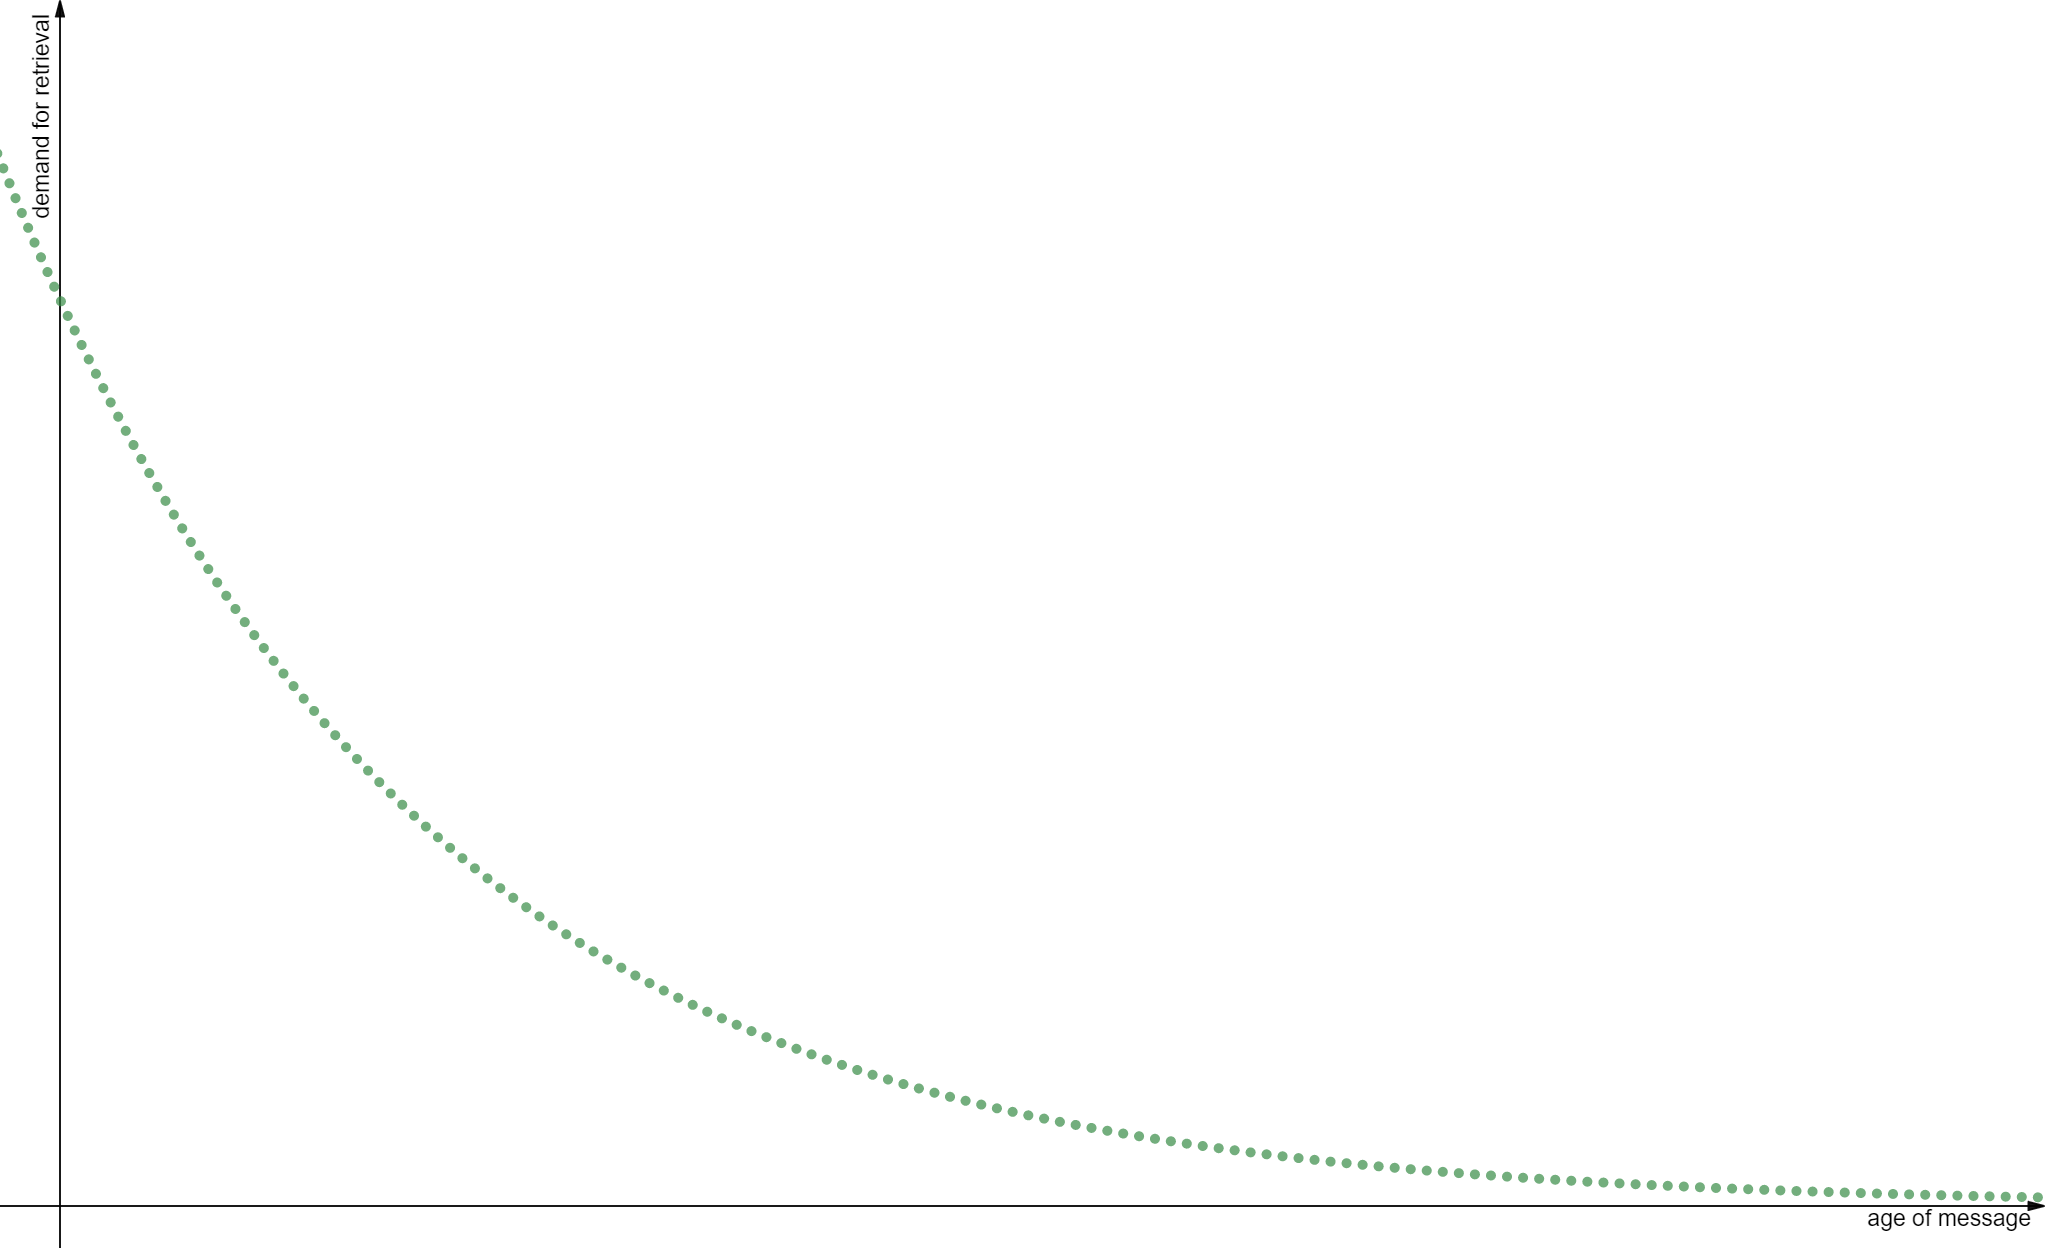
\includegraphics[width=0.7\linewidth]{Images/exponential.PNG}
    \caption{An approximation of demand for message retrieval against age of messages.}
    \label{fig:exponential_vague}
\end{figure}

We can model the probabilities in a Probability Distribution Function ($p.d.f.$). The following is an exponential graph which models transactions and blocks continuously despite the fact that they are really discrete.
\[ \]
\[p.d.f. = f(t) = 
\begin{cases}
        k \cdot m^{t} &0 \leq t \leq 1, \\[6pt]
        0 &\textrm{otherwise.}
    \end{cases}
\]
where
\begin{align*}
    \begin{cases}
        k &\coloneqq \dfrac{\ln{m}}{m-1} \\[6pt]
        m &\coloneqq \textrm{Factor indicating client's preference on storing older to newer messages.} \\[6pt]
        t &\coloneqq \dfrac{\textit{Current block number - Specified block number}}{\textit{Current block number}} \\[6pt]
    \end{cases}
\end{align*}
and
\[
0 \leq t \leq 1, \hspace{0.25cm}
m > 0, \hspace{0.25cm}
m \not= 1
\]

To calculate the probability that a block should be stored, the following formula could be used.
\[
p_t = \max\left(\dfrac{k \cdot m^t \cdot \textit{Remaining block storage capacity}}{\textit{Current block number} + 1}, \hspace{0.1cm} 1\right)
\]

This will increase the probability of storing a block based on how much storage the client has remaining. With this system, if the client has lots of available storage then they will almost certainly store a received block.

\newpage

\subsubsection{Node Tiers}

I propose that my implementation would have four tiers of network nodes ranging from \textit{archival nodes} to \textit{thin nodes}.

\begin{center}
    \Large{\textit{archival nodes}}
\end{center}

I define archival nodes as any nodes that prefer the storage of older messages to newer messages (ie. $m > 1$). This type of node is run by those who wish to keep a deep record of the blockchain. They will typically have a large amount of available storage and serve a useful purpose for those who need to access older messages. A \textit{full archival node} stores the entire blockchain all the time and a \textit{semi-archival node} stores only parts of the blockchain (still preferentially stores older blocks over newer).

\textit{Full archival nodes} will be able to validate blocks with absolute certainty since they have immediate access to the entire blockchain. \textit{semi-archival nodes} will have less certainty since they have access to fewer blocks in the blockchain.

\begin{center}
    \Large{\textit{neutral nodes}}
\end{center}

I define neutral nodes as nodes that support the network by storing blocks according to demand. This means that they preferentially store newer blocks over older blocks. Most of the nodes on the network should be neutral nodes of some kind. Thinner neutral nodes will store fewer blocks overall but still in the same proportions (according to the curve above). The bulk of nodes on the network should be neutral nodes since this will provide the best access speeds for others.

This kind of node will be able to validate blocks with almost exact certainty as they have nearly all of the recent blocks and all of the block headers.

\begin{center}
    \Large{\textit{thin nodes}}
\end{center}

Thin nodes are those which store almost none of the blockchain themselves; instead they rely on others in the network to provide valid blocks. This kind of node should only be run by devices with very limited resources such as embedded devices.

This kind of node will not be able to validate blocks with as-high certainty since few blocks are stored. This type of node relies on the consensus of different network nodes (ie. queries several different nodes to confirm the legitimacy of blocks). This kind of node will not benefit the network since it doesn't provide the same services as \textit{neutral} and \textit{archival} nodes.

\vspace{1cm}
Whilst these kinds of nodes are fairly comprehensive, there will always be nodes who switch between being \textit{archival} and \textit{thin} etc. These definitions are purely for convenience and don't intend to impose any rules on the clients.

\normalsize

\subsubsection{Attractive Addressing}
Although addresses are fairly core to the project, I would still classify them as implementation details since they can easily be redesigned/reimplemented in another format. Also note that these addresses are different to the `address' data type which is used by the network protocol. The following refer to what users will see and show to their friends and not what the network will encode into a transaction.

If distributing and communicating addresses is too difficult then the platform will become unusable for many people. It is therefore vital that addressing is made as simple as possible. For this reason, I have followed in Bitcoin's footsteps by using base58 encoding for addresses. This is an alternative to base64 encoding that avoids characters which may appear similar in some fonts. The Bitcoin documentation contains the following reasons for the choice to use base58.
\begin{minted}{rust}
    // Why base-58 instead of standard base-64 encoding?
    // - Don't want 0OIl characters that look the same in some fonts
    //      and could be used to create visually identical looking 
    //      account numbers.
    // - A string with non-alphanumeric characters is not as easily
    //      accepted as an account number.
    // - E-mail usually won't line-break if there's no punctuation
    //      to break at.
    // - Doubleclicking selects the whole number as one word if 
    //      it's all alphanumeric.
\end{minted}
Clearly, all these reasons still apply to this platform and therefore base58 is a good choice.

This system, however, is still rather unwieldy. For many people, the very idea of an address---username if you will---being a long string of alphanumeric characters will be off-putting. This may make them resort to sending their address over another messaging platform---effectively rendering many of the platform's anonymity benefits pointless. For this reason, it is important that there is a simpler way for users to communicate their addresses. A simple and effective solution is the `QR Code' (Quick Response code; as seen in \autoref{subsubsec:qrcodes}). This would allow users to quickly show their friends a visual code on their device reducing the need for a messenger service to be used for communicating addresses. For the highest security, all addresses should obviously be communicated in person, away from any potential onlookers. However, in the event that an address was correctly linked with a human, the messages would still be cryptographically secure.

The other problem with addresses which are long strings of characters is the difficulty for humans to differentiate between addresses for different platforms. By this, I mean that it is hard to see a long string of characters and immediately work out that it is an address for this platform and not some other (eg. a bitcoin wallet address). To fix this, I am prepending the short string ``Bim''\footnote{If it's unclear, then ``Bim'' stands for Blockchain Instant Messaging/Messenger.} to the beginning of an address. This should make it very clear which platform an address belongs to. A similar `magic' is prepended to Bitmessage addresses, `BM-'. However, the dash reintroduces problems when doubleclicking and in an email; thus, I decided to remove it for my implementation.

Also important is versioning of addresses. As this implementation progresses, there will likely be changes to address structure over time leading to non backward-compatible modifications. This means that it is necessary to have a version encoded in the address.

The steps to generate a \textbf{Bitmessage} address are as follows\cite{bitmessage_address}:
\begin{enumerate}
    \item Create a private and a public key for encryption and signing (resulting in 4 keys)
    \item Merge the public part of the signing key and the encryption key together. (encoded in uncompressed X9.62 format) ($A$)
    \item Take the SHA512 hash of A. ($B$)
    \item Take the RIPEMD160 of B. ($C$)
    \item Repeat step 1-4 until you have a result that starts with a zero (Or two zeros, if you want a short address). ($D$)
    \item Remove the zeros at the beginning of D. ($E$)
    \item Put the stream number (as a var\_int) in front of E. ($F$)
    \item Put the address version (as a var\_int) in front of F. ($G$)
    \item Take a double SHA512 (hash of a hash) of G and use the first four bytes as a checksum, that you append to the end. ($H$)
    \item base58 encode H. ($J$)
    \item Put ``BM-'' in front J. ($K$)
\end{enumerate}
$K$ is your full key.

I can modify the Bitmessage approach above for this project. This will involve three main changes. The first is removing the key for signing.

\subparagraph{Separate Keys for Encryption vs Signing}
Bitmessage separates the key pairs used for encryption and signing. This has several benefits, mainly boiling down to the ability for an encryption key to be compromised without the signing one being compromised. In other words, if a victim user's encryption key is compromised, then it remains impossible for an attacker to impersonate the victim so long as the signing key is still secure. This is obviously very useful and also functions as a way for businesses and other organisations to share messages without distributing the ability to send messages. Whilst this would be a very useful feature for the platform---one that should be added in future iterations if possible---it adds extra complexity at this point and would involve a fair redesign of much of the platform. I leave this to possible future versions of the standard and so, for now, this platform will only make use of one key pair per user for both encryption and signing.

\subparagraph{RIPEMD160 and Hashing} The second moodification is to the hashing algorithm. Bitmessage's addresses (and Bitcoin's for that matter) are computed by hashing some configuration of the user's public key using SHA512 and RIPEMD160 (160-bit RIPE message digest). This distances users' public keys from their actual addresses. There are some good reasons for doing this (see \autoref{subpara:addrsvspubkeys}); however, I don't think it is necessary for the platform and thus I will remove this from the address generating algorithm.

\subparagraph{Stream Numbers} Stream numbers are a feature of Bitmessage that remain almost unused since they were first suggested in the Jonathan Warren's Bitmessage paper\cite{bitmessage_paper}. The idea is to help with scalability allowing nodes to `cluster' into groups (streams) to restrict network traffic to certain groups, reducing the overall traffic. Whilst this was a good idea and is relatively easy to implement, it has never been properly used to the best of my knowledge. By default, Bitmessage addresses use 1 for their stream numbers and there has never been a significant reason not to. Since this is a feature which is not strictly necessary (possibly even quite unnecessary), I have decided to strip this from the creation of an address.


After these modifications, I am left with the following steps.
\begin{enumerate}
    \item Create a single private and a public key pair for encryption and signing (resulting in 2 keys)
    \item Convert public key to data type `address'. ($A$)
    \item Put the address version (as a char[\hspace{0.05cm}]) in front of $A$. ($B$)
    \item Take a double SHA512 (hash of a hash) of $B$ and use the first four bytes as a checksum, that you append to the end. ($C$)
    \item base58 encode $C$. ($D$)
    \item Put ``Bim'' in front $D$. ($E$)
\end{enumerate}
$E$ is your Blockchain Instant Messaging/Messenger address.

Note that, I have decided to keep the checksum. This is for good reason as it provides a way of validating the integrity of an address when transferred between two people (eg. misread QR Code). I have also decided to change the data type of the address `version'. This was done in order to align the addressing system with the network protocol. Also, it's worth noting that not all addresses will be the same character length since different versions will require different numbers of bytes to function as well as the base58 function creating strings of different lengths.

\subparagraph{Deterministic Addresses}
The ability to create deterministic addresses is a feature of many Bitcoin and Bitmessage clients. It allows a user to remember some passphrase which acts as a seed to create a private key and from there a public key. It's a useful feature for a lot of people as it means that they neither have to remember a long string of seemingly random characters nor do they have to go through a complex process of transferring their keys between clients. 

Deterministic addresses often come with a lot of security vulnerabilities\footnote{An excellent talk\cite{defcon_22} from Defcon 22 lays out not just why they can be insecure but also how they can be improved.}. However if a user is careful, then they can be extremely helpful.

\vspace{1cm}
This concludes the set of details which I believe are important for an implementation of this project.


%%%%%%%%%%%%%%%%% PoC %%%%%%%%%%%%%%%%%


\newpage
\section{Proof of Concept}
This project would seem incomplete if I were not to at least attempt to prove the concept. Therefore, I have worked on a few program snippets that demonstrate key elements of the platform. For example, I have prepared a demo of a client serialising a set of blocks to a `blocks' network request.

For the purposes of the following demonstrations, I have chosen the programming language \textbf{rust}. Rust would be a good choice for a `core' client implementation since it is a compiled language (generally faster than an interpreted one) and it is designed to be `safe' (not vulnerable to buffer overflows and use-after-free issues). More information can be found on the language here\cite{rustlang}. However, rust is not readily used for UI or mobile application programs which could make it an undesirable language choice for some implementations.

\subsection{Structures}
\begin{minted}{rust}
/*
 * Note that there is no in-built 256-bit integer in 
 * rust and therefore, I define the `tx_id' as a vector of bytes.
 * I also never explicitly define the `address' type here but
 * this would have to be implemented.
 */
struct Tx {
    version: Vec<char>,
    tx_id: Vec<u8>,
    lock_time: u32,
    nonce: u64,
    tsdc: u64,
    iv: Vec<u8>,
    r: Address,
    encrypted_payload: EncryptedPayload,
}

/* 
 * The type `VarUInt' is not present in vanilla rust.
 * It would have to be implemented separately.
 */
struct EncryptedPayload {
    msg_id: VarUInt,
    tx_from: Address,
    tx_to: Address,
    msg_sig: Vec<u8>,
    msg_type: u8,
    msg: Msg,
}
\end{minted}

\begin{minted}{rust}
/* 
 * The message types could be implemented as follows.
 * Here, I define a Msg as an `enum'.
 */
enum Msg {
    Text(MsgText),
    Acknowledgement(MsgAcknowledgement),
    Sticker(MsgSticker),
    Reaction(MsgReaction),
    File(MsgFile),
    Poll(MsgPoll),
    PollVote(MsgPollVote),
    SetNickname(MsgSetNickname),
    SetChatname(MsgSetChatname),
}

/* 
 * Whilst I won't go through every kind of message here,
 * it would be trivial to extend this to include all
 * message types.
 */
struct MsgText {
    encoding: Encoding,
    data: Vec<u8>, 
} // Here, data could potentially be stored as a String.

struct MsgAcknowledgement {
    rmsg_id: VarUInt,
}

struct MsgSticker { ... }
struct MsgReaction { ... }
struct MsgFile { ... }
struct MsgPoll { ... }
struct MsgPollVote { ... }
struct MsgSetNickname { ... }
struct MsgSetChatname { ... }
\end{minted}

\newpage

\begin{minted}{rust}
/* 
 * The structure of a block is defined in just the same
 * way.
 */
struct Block {
    version: Vec<char>,
    no: u32,
    block_id: Vec<u8>,
    prev: Vec<u8>,
    nonce: u64,
    ts: u32,
    tx_l: Vec<Tx>,
}

/*
 * This shows how the designed data structures could be
 * translated into code in a client implementation.
 */
\end{minted}

\newpage

\subsection{Serialisation}
\begin{minted}{rust}
/*
 * The following code shows how a block could serialised
 * into a network request.
 * In rust we can create a trait that allows for quick
 * conversion from a vector of blocks to a `blocks' request.
 */
trait ToBlocksRequest {
    fn to_blocks_request(&self, network: Network) -> BlocksRequest;
}

impl ToBlocksRequest for Vec<Block> {
    fn to_blocks_request(&self, network: Network) -> BlocksRequest {
        magic: network.magic,
        command: "blocks",
        checksum: sha256(&self),
        payload: &self,
    }
}
\end{minted}

\newpage

\begin{minted}{rust}
/*
 * Now we can serialise this request into bytes to be sent
 * over the network.
 * I am not going to show the exact conversion from vectors
 * to bytes but it wouldn't be difficult to implement.
 */

/*
 * Below is an example of a serialised `blocks' request
 * in hex.
 *
 * DDE6AE4C             // Main network magic
 * 0006626C6F636B73     // command string ``blocks''
 * 9CEB48F4             // 4 byte checksum value
 *   0002                 // 2 blocks in this request
 *   // First block //
 *   000676302E302E31     // version string (length 5)
 *   0000000000000001     // block number = 1 (second block)
 *   F42298FE25B96AB6...  // 256-bit merkle
 *   00ECEB66FFC86F38...  // BlockID of previous block
 *   696C79C2DBC239DD4E91B46729D73A27 // nonce
 *   5E831406             // 32-bit unsigned UNIX timestamp
 *     001E                 // 30 tx's in this block
 *     // First tx //
       000676302E302E31
 *     ...
 *   ...
 * ...
 *
 * Note that the newlines here are not present in an actual
 * request. All data is concatenated.
 */

\end{minted}

\newpage

\subsection{Networking}
\begin{minted}{rust}
/*
 * The following code shows how a very basic TCP client
 * could be created and used to send a Network request to a
 * node.
 */

use std::net::{TcpStream};
use std::io::{Read, Write};

fn main() {
    
    ...
    
    match TcpStream::connect("some_ip_and_port") {
        Ok(mut stream) => {
            let req = some_request.as_bytes();

            stream.write(req).unwrap();

            let mut data = [0 as u8; 6];
            match stream.read_exact(&mut data) {
                Ok(_) => {
                    println!("Received reply: {}", 
                        Request::from_bytes(&data));
                },
                Err(e) => {
                    printerr!("Failed to receive data: {}", e);
                }
            }
        },
        Err(e) => {
            printerr!("Failed to connect: {}", e);
        }
    }
    
    ...
    
}

\end{minted}

\newpage

\subsection{Example Address Generation}
\begin{minted}{rust}
/*
 * Below is an example implementation of the conversion
 * from public address components to the `address' type.
 */

struct Address {
    a: Vec<u8>
}

impl Address {
    fn from_pubkey(x: &Vec<u8>, y: &Vec<u8>) -> Address {
        let odd_or_even = match y.last().unwrap() % 2 {
            0 => 0u8,
            1 => 255u8,
            _ => panic!("Even / Odd check failed!"),
        };
        
        let mut addr = x.clone();
        addr.push(odd_or_even);
        
        Address { a: addr }
    }
}

\end{minted}

\newpage

\subsection{UI Design}
A project like this would seem incomplete if I weren't to design a mock up user interface. For this, I used Google's Flutter framework\cite{flutter_framework} with the Dart programming language\cite{dart_lang}.

For demonstration, I branded the `implementation' as `chains'.

\vspace{0.8cm}

\noindent
\begin{center}
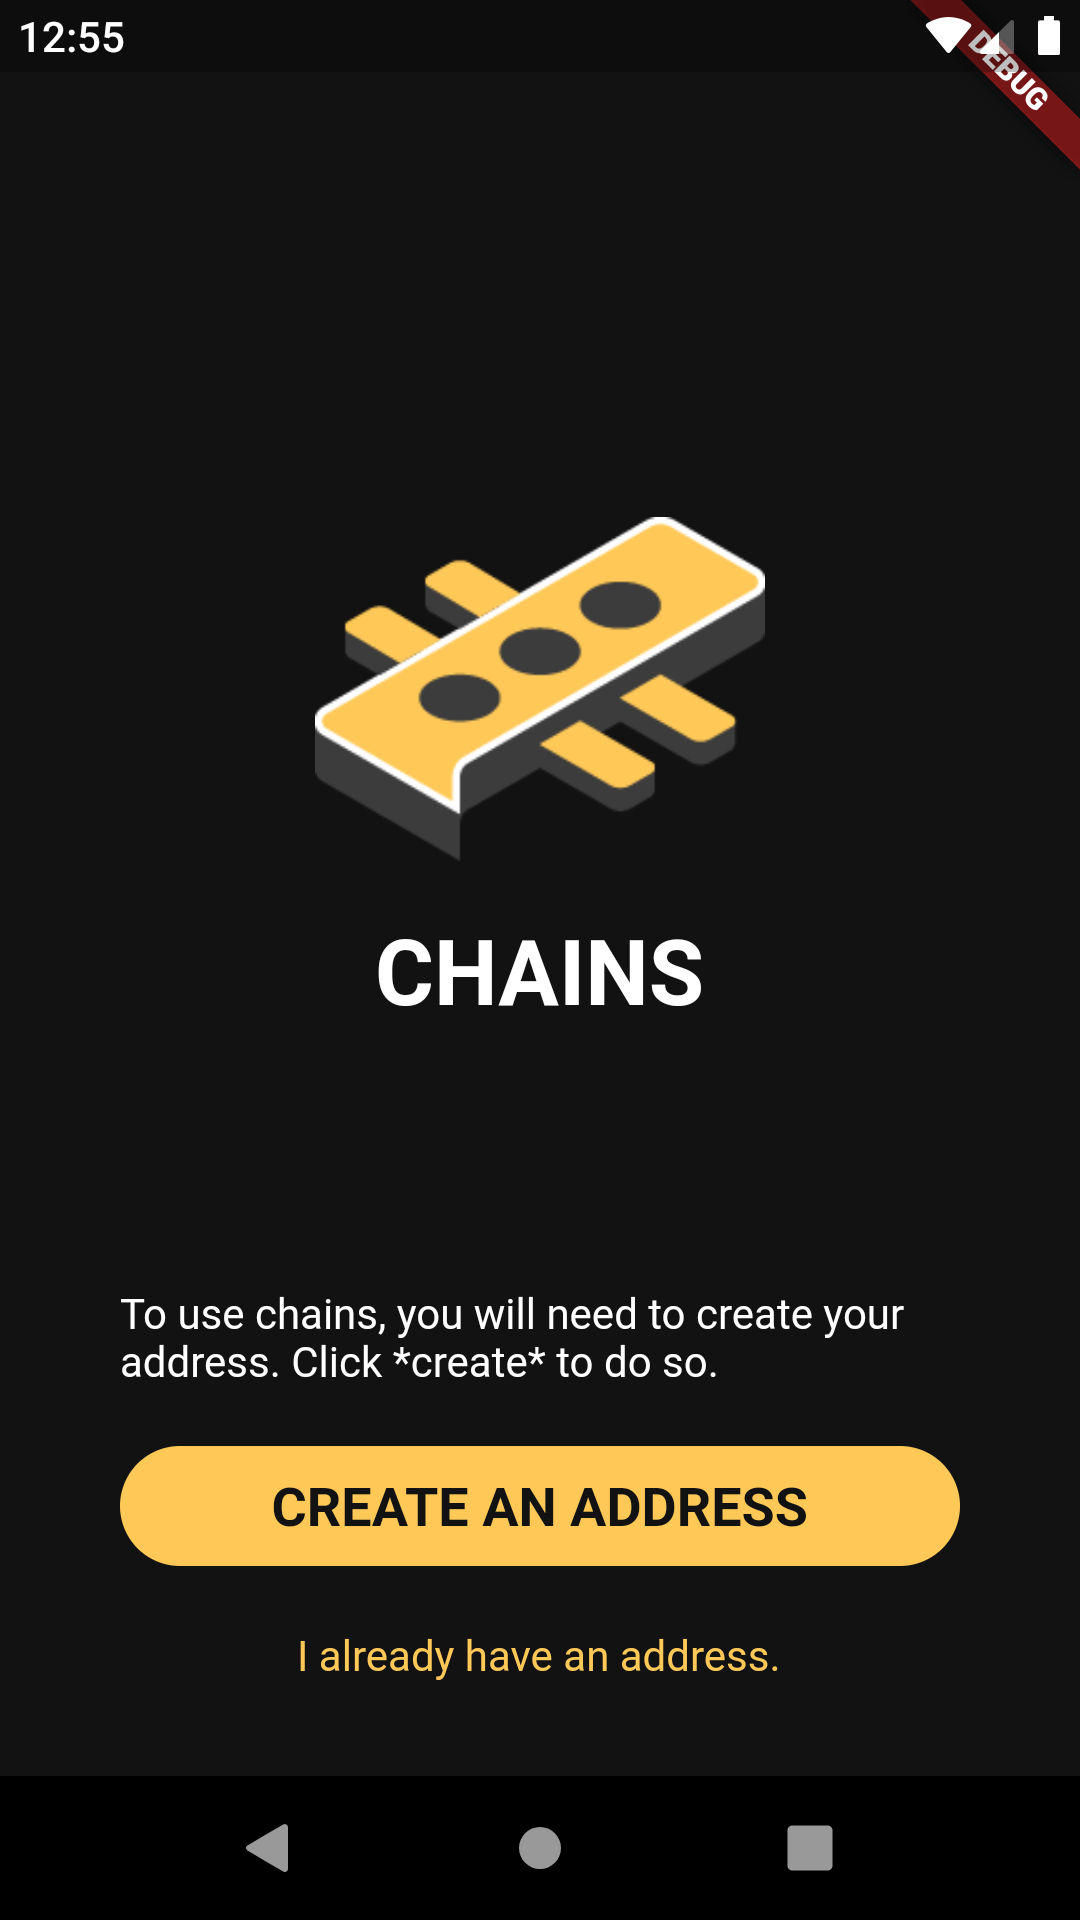
\includegraphics[width=0.33\textwidth]{Images/chains_1.png}\hspace{0.1\textwidth}%
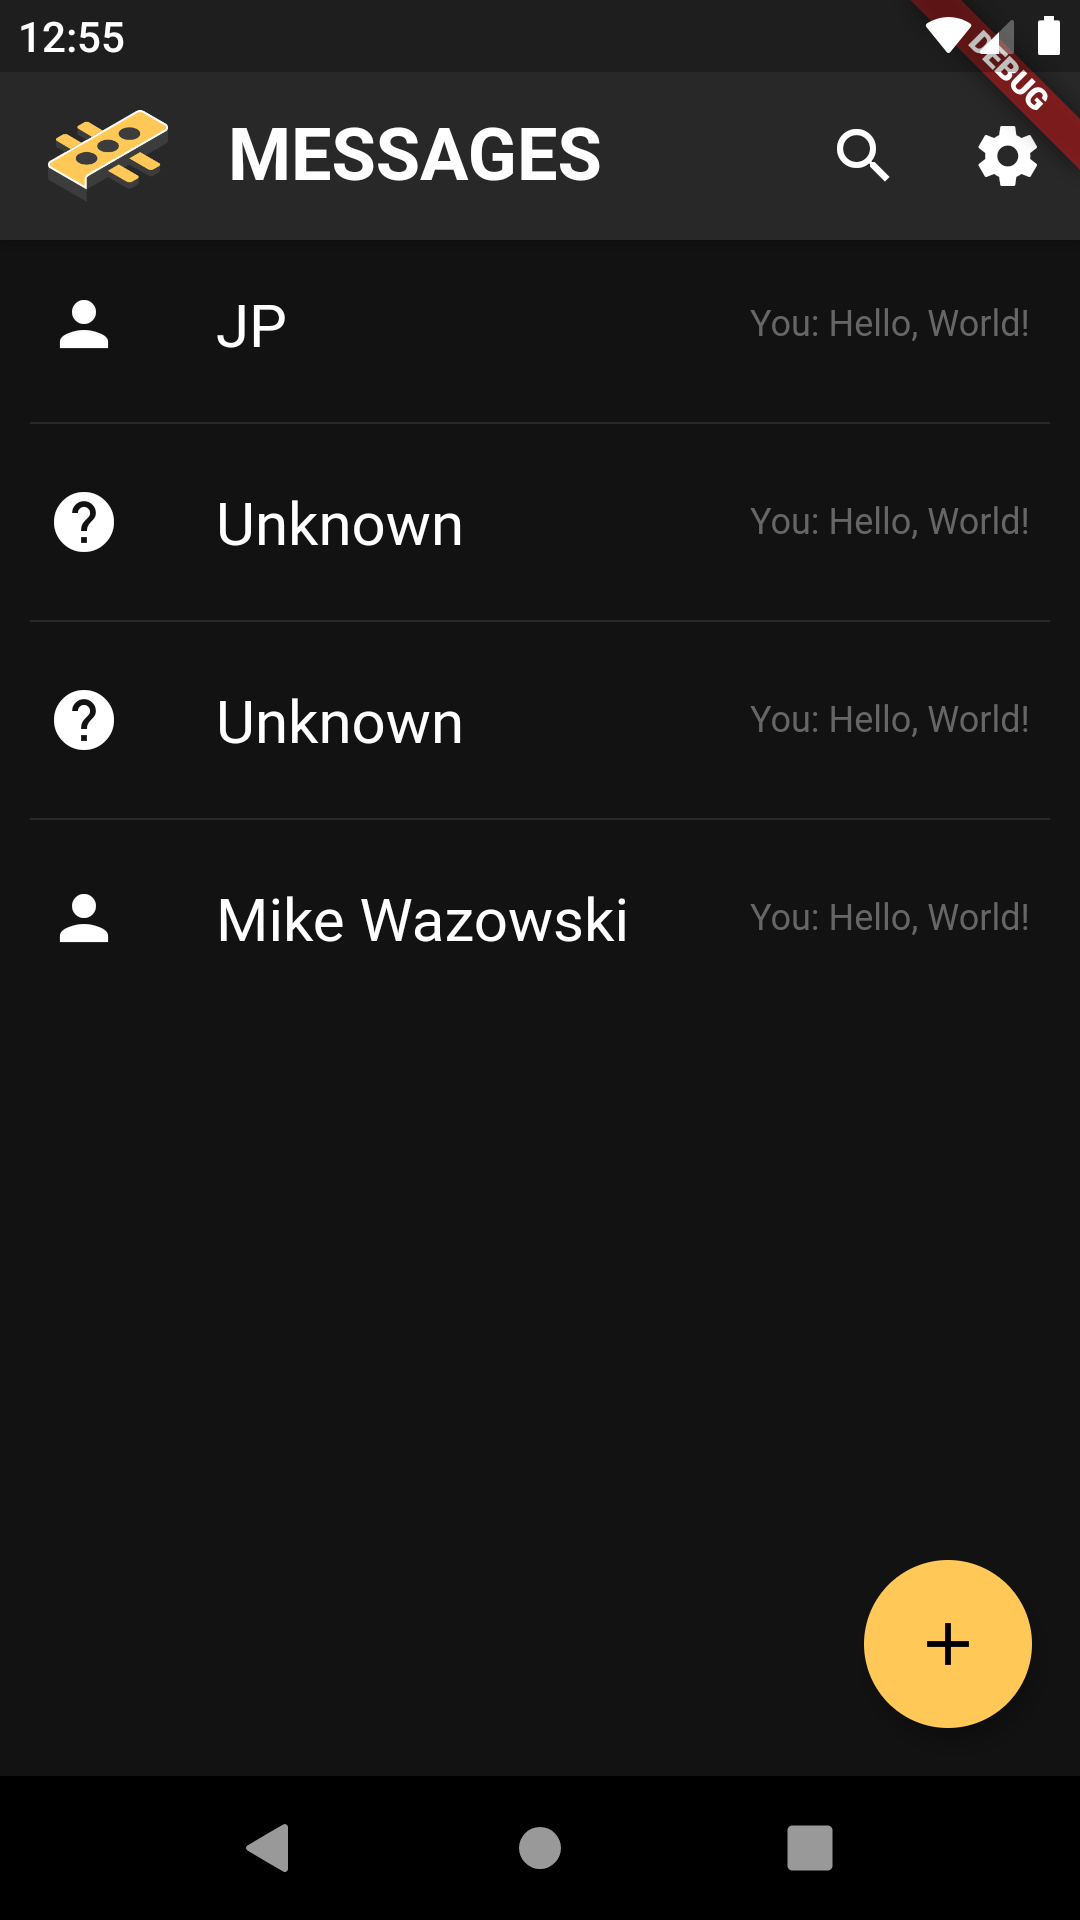
\includegraphics[width=0.33\textwidth]{Images/chains_2.png}\\[2em]
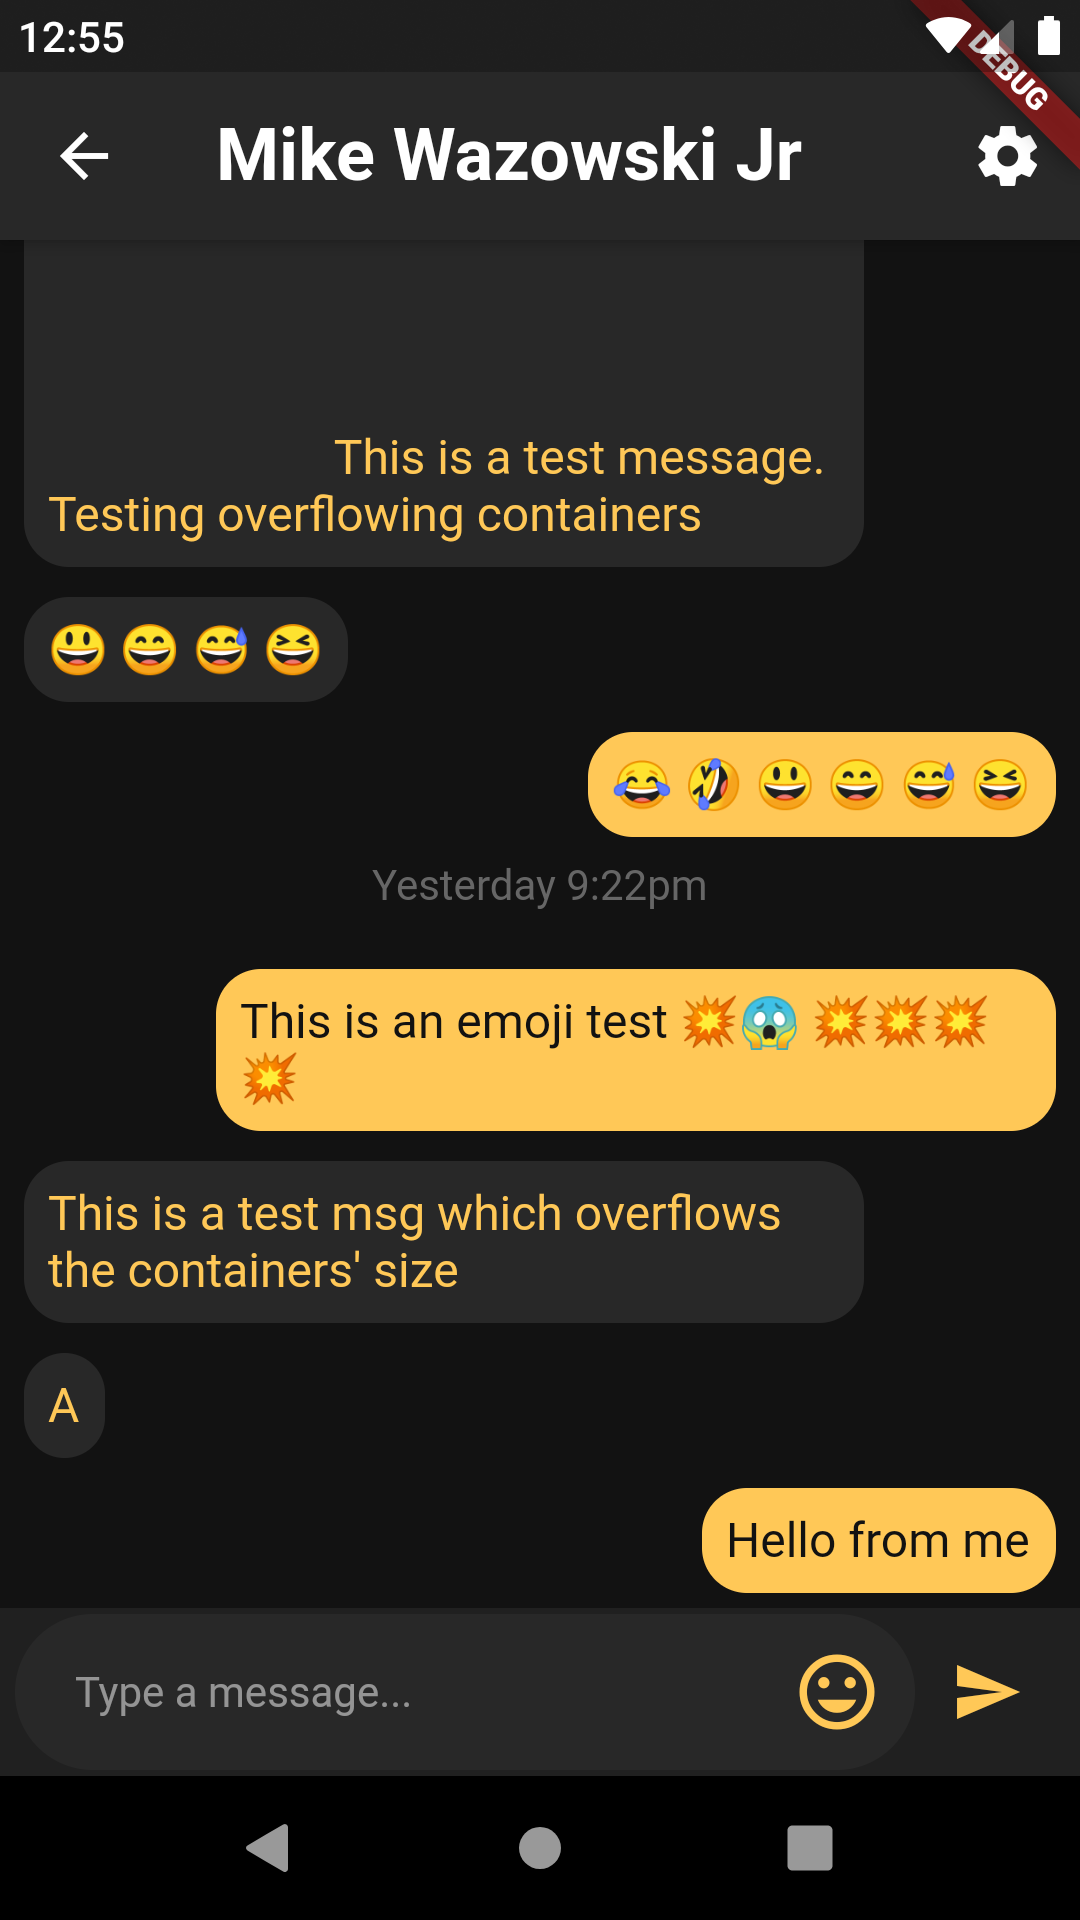
\includegraphics[width=0.33\textwidth]{Images/chains_3.png}\hspace{0.1\textwidth}%
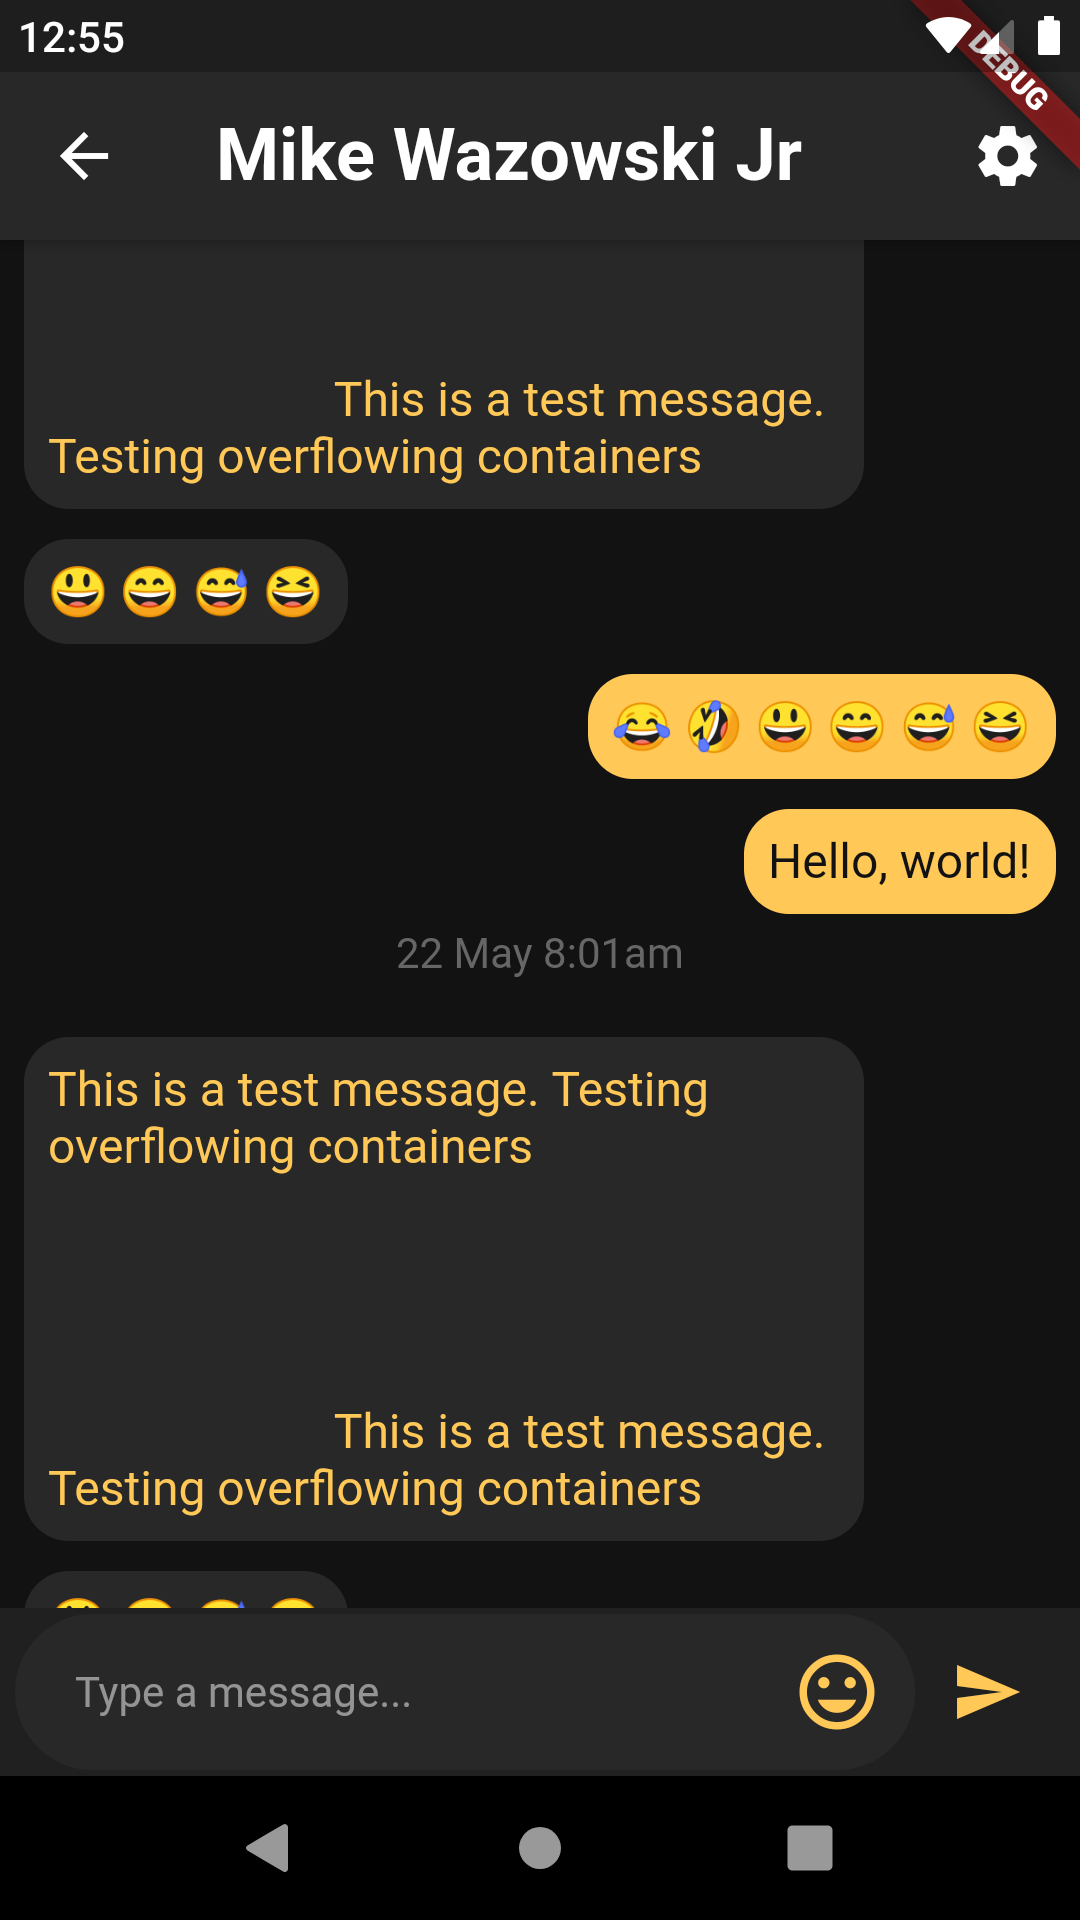
\includegraphics[width=0.33\textwidth]{Images/chains_4.png}\par
\end{center}

\clearpage

\section{Evaluation}
When theorising this project in the very beginning, I aimed to create a detailed, informative and advanced specification for an instant messaging platform that runs in the blockchain. I believe that I have achieved this. I was able to create a second revision (\textit{v2}) of the platform that fixed many of the oversights of the first. Once I had created this revision, I was able to attempt to implement parts of the project. I believe that these snippets successfully proved the concept of the platform and complemented the artefact well.

However, during the process of researching and designing for this project, I encountered several, major setbacks. These largely comprised of errors in time management.

\subsection{Time Management}
Of all the problems encountered in the course of this project, the greatest barrier by far was time management. On my research project alone, I ended up finishing over two weeks behind my initial aims. I ended up spending the vast majority of my time on designing the platform which is how I would have liked it but, in the end, I spent too long on design and it cost me in the later stages when I felt more pressured and became less productive. Early on I should have been more open to dropping unnecessary parts of the projects such as `block authors' (see \autoref{para:block_authors}). Not only was the `block authors' feature unnecessary but actually the way I wanted to implement it was majorly flawed.

During the design section of the process, I found it very difficult to stay up to date with my activity log whilst also keeping up progress on the project itself. In hindsight, the activity log was very useful when I did keep it up to date, because it helped me to work out which ideas mattered to the project, and what I should focus on doing during the next week.

Sporadically, throughout the entire process, I found myself paying too much attention to the typesetting and layout of my report. Whilst I still think that this is important in many ways, I realise now that I should have spent less time on it in the moment and left the aesthetics until the end. Often I would find myself tweaking a paragraph early in the report and messing up the typesetting of one of the following pages. I would then proceed to spend half an hour rearranging paragraphs only to repeat the same mistake just days later. The time lost from mistakes like this could have been spent on further implementing the project or introducing more useful features into the platform itself. However, in my opinion, I \textit{would} say that the typesetting and layout of the final report worked out well in the end.

\subsubsection{Improvements}
To improve my time management, I should have definitely, always kept my activity log up to date. This would have been easy to do and would have improved the quality of the project as a whole because I would have been more focused and organised. My Gantt charts should have been more detailed and well-thought-through as this would have avoided the increased pressure and stress towards the end of the project. I also could have better defined the scope of the project at the start as this would have meant I wasted less time researching topics that were largely irrelevant to the core of the platform.

\subsection{Main Goal}
In terms of achieving a fully anonymous instant messaging platform, I believe that I have been very successful. This project was able to design a platform which could improve the lives of many people, providing anonymity to some who are living under oppressive regimes or simply want to avoid the arguable data-hoarding of large businesses such as Facebook. It's worth noting that there may be some fatal flaw in the design of this platform that makes it unusable or insecure. Even if this is the case, I am still pleased with the design which I was able to put together.

As mentioned in `Ethics' (\autoref{subsec:ethics}), there would be drawbacks concerned with implementing a project such as this. Most notably, the ability for criminals to communicate freely without fear, not to mention the impacts on climate change of potentially thousands of machines mining for blocks. I still believe, however, that this project does more good than bad.

As long as this project is only on paper, though, it is not helping anyone and in the future I hope to implement the project to the best of my ability.

\subsection{Conclusion}
Although this project may have required considerable effort and time, I am very happy with the work I have been able to achieve on this and it has taught me much about organisation; time management; planning; research; and of course blockchain, cryptography and networking.

\clearpage
\printbibliography

\vspace{6.5cm}

\begin{center}
    \textbf{Jasper Parish\\2020}
\end{center}
\end{document}